\cleardoublepage
% 数字字体不统一

% 标示时间、空间、序数等项目的起止,连接相关名词表示走向,在标准编号中连接顺序号与年号等情况下,应当使用一字线(—);标示数值范围时应当使用浪纹线(~);在电话号码、门牌号、图表编号、阿拉伯数字年月日等各种复合名词及外来语内部分合中起连接作用时,应当使用短横线(-)。例如:
% 时间起止(一字线):鲁迅(1881—1936)2016—2020年 1—3月 10月1日—7日 上午8:00—12:00
% 空间起止、走向(一字线):北京—上海特快列车 秦岭—淮河线
% (表示时间或者空间起止,通常用一字线;其中表示范围的,有时也可用浪纹线)
% 序数起止(一字线):1—5号楼 第21—30条
% (当序数起止表示的是数值范围时,也可用浪纹线,如:第5~8课)
% 标准编号(一字线):GB/T 15834—2011《标点符号用法》
% (一字线还可以表示递进、发展等关系)
% 数值范围(浪纹线):25~30 g 6%~8% 3~5年内
% (表示数值范围,通常用浪纹线,有时也可用一字线)
\section{实验思路和设计} 
\subsection{实验总体设计}

\subsection{实验材料、仪器与软件}
\subsubsection{实验材料}
\begin{enumerate}
    \item \textbf{蔗糖酶的提取和粗分离:}市售干面包酵母粉,石英砂,Tris-Cl pH7.4缓冲液,95\%乙醇溶液
    \item \textbf{阴离子交换柱色谱:}DEAE-Sepharose Fast Flow 树脂,0.5mol/L NaOH,0.5mol/L NaCl溶液,缓冲液 A(20 mmol/L Tris-Cl, pH7.4),缓冲液 B(0.5 mmol/L NaCl + 20 mmol/L Tris-Cl, pH7.4)
    \item \textbf{蔗糖酶活性检测:}5 \%蔗糖溶液,0.1 mol/L 乙酸缓冲溶液(pH4.6),3,5-二硝基水杨酸(DNS)试剂
    \item \textbf{蛋白质浓度测定:}0.5g/L 血清白蛋白溶液,Folin-酚试剂甲,Folin-酚试剂乙
    \item \textbf{葡萄糖标准曲线:}1g/L 葡萄糖标准溶液,3,5-二硝基水杨酸(DNS)试剂
    \item \textbf{蔗糖酶酶切去糖基化:}0.1mol/L pH5.6 乙酸钠缓冲液,1 U/μl Endo H
    \item \textbf{SDS-PAGE:} 30\%凝胶贮液,3mol/LTris-HCl pH8.9 分离胶缓冲液,1mol/L Tris-HCl pH6.7 浓缩胶缓冲液,10\% SDS,TEMED,10\% Ap,MARKER,考马斯亮蓝快速染色液
    \item \textbf{糖蛋白电泳:}30\%凝胶贮液,3mol/LTris-HCl pH8.9 分离胶缓冲液,1mol/L Tris-HCl pH6.7 浓缩胶缓冲液,10\% SDS,TEMED,10\% Ap,10 \%三氯乙酸,1 \%高碘酸溶液,0.1 \%偏重亚硫酸钠溶液,品红染色溶液,7\%乙酸溶液
    \item \textbf{活性蛋白电泳:}30\%凝胶贮液,3mol/LTris-HCl pH8.9 分离胶缓冲液,1mol/L Tris-HCl pH6.7 浓缩胶缓冲液,10\% SDS,TEMED,10\% Ap,0.1\%Triton X-100溶液,含5\%蔗糖的0.1mol/L乙酸缓冲液(pH4.6),0.1  mol/L碘乙酰胺,含0.2\%(w/v) TTC 的0.5mol/L  NaOH 溶液,7.5\%乙酸
    \item \textbf{Western Blot:}30\%凝胶贮液,3mol/LTris-HCl pH8.9 分离胶缓冲液,1mol/L Tris-HCl pH6.7 浓缩胶缓冲液,10\% SDS,TEMED,10\% Ap,PVDF膜,含5\%脱脂奶粉的TBST缓冲液(1L含0.1\%吐温-20,Tris 1.21g,NaCl 4g,pH7.6),辣根过氧化物酶(HRP)标记的二抗,蔗糖酶一抗、含碱性磷酸酶标记的二抗、TMB 显色剂
    \item \textbf{动力学测定:}DNS 试剂,5\%蔗糖,0.5g/L 葡萄糖标准溶液,0.1 mol/ L 乙酸缓冲液, pH=4.6,4 mol/L 尿素溶液
\end{enumerate}
% 10 \%葡萄糖溶液、pH5.6 乙酸钠缓冲液、Endo H 试剂、30\%凝胶贮液(Acr + Bis)、3 mol/L Tris-HCl
% pH8.9 分离胶缓冲液、1 mol/L Tris-HCl pH6.7 浓缩胶缓冲液、、、
% 考马斯亮蓝快速染色液、希夫试剂染色与脱色(10 \%三氯乙酸、1 \%高碘酸溶液、0.1 \%偏重
% 亚硫酸钠溶液、品红染色溶液)、甲醇、5 \%脱脂奶粉、TBST 缓冲液、

\subsubsection{实验仪器}
% 直接补充
研钵,电子天平,差速离心机,涡旋仪,实验室蛋白质层析系统AKTA Start,恒温水浴箱,紫外-可见分光光度计,摇床,蛋白电泳槽系统。

\subsubsection{实验软件}
\begin{enumerate}
    \item AKTA Start
    \item Origin 2023
    \item GelAnalyzer 
    \item PyMol
    \item ChemDraw 
\end{enumerate}

\subsection{实验方法和原理}

\subsubsection{蔗糖酶的分离与纯化}
从蔗糖酶中提取蔗糖酶并进行粗分离涉及到破碎、热处理、乙醇沉淀和复性溶解四个过程。通过石英砂研磨破碎的方式,可将包括蔗糖酶在内的丰富蛋白质从细胞中分离并溶解到缓冲液中,随后通过离心法将不溶的残渣及脂质分离去除。为了实现高效选择性沉淀,我们采用了热处理和乙醇沉淀两种方法。由于目标蔗糖酶在50\dc 下保持相对稳定,将溶液加热至50\dc ,在保证酶活性不发生改变的前提下可以沉淀高温下不稳定的杂质蛋白质。同时,通过乙醇处理,蛋白质发生变性并沉淀,而蔗糖酶在乙醇沉淀后后仍然具有复性能力。用乙醇使溶液中的蛋白质变性,离心分离并去除上清液,随后用新的缓冲液溶解,无法复性的杂质蛋白质因而被有效去除。

为了分离纯化蔗糖酶,采用离子交换层析纯化。离子交换层析,又称离子交换色谱,以离子交换剂作为固定相,通过可逆交换结合力的差异来实现成分离子的分离。在特定pH值的溶液中,不同等电点的蛋白质带有不同电荷,因此与离子交换剂的亲和力也存在差异。透过调整洗脱液的pH或逐渐增加盐的离子强度,使特定蛋白质的电荷发生改变,进而改变其与离子交换剂的亲和力,不同带电荷的蛋白质可逐一被洗脱。部分收集截取梯度洗脱中的洗脱峰溶液,不同收集管中包含了不同的蛋白质,从而达成分离目的。离子交换层析具有分析速度快、灵敏度高、选择性好、浓缩效应显著、同时分析多种离子等优势。

\subsubsection{纯化方案评价}
经过分离纯化得到的蔗糖酶的纯度、比活力、回收率和离子交换色谱综合洗脱曲线是纯化方案质量评价的基本技术指标。因此,我们需要定量测定蛋白质浓度并定量检测蔗糖酶的活性,同时建立离子交换色谱的综合洗脱曲线。

 \noindent \textbf {1. 蛋白质浓度的测定}
 
自然界中蛋白种类多达$10^{12} \sim 10^{14}$种,其组成、结构、大小、特征与性质相差巨大,测量中还存在不同的杂质干扰,因此从来没一个理想又通用的蛋白质定量分析方法。长期以来,科学家们主要基于蛋白质与铜离子螯合或染色特性创建了许多方法来进行定量测定。为某个具体的样本选择一个合适的蛋白定量测定方法一直困扰着科学界。

\begin{table}[H]
\centering
\caption{蛋白质定量测定的方法}
\label{tab:my-table}
\begin{tabular}{@{}cccc@{}}
\toprule
\multirow{2}{*}{直接测定} &
  \multicolumn{3}{c}{间接测定} \\
 &
  吸附性 &
  螯合性 &
  化学性质 \\ \midrule
\begin{tabular}[c]{@{}c@{}}紫外吸收法\\ 质谱法\end{tabular} &
  \begin{tabular}[c]{@{}c@{}}氨基黑法\\ 考马斯亮蓝法\\ 银染法\end{tabular} &
  \begin{tabular}[c]{@{}c@{}}荧光法\\ Western Blot\\ 酶标法\end{tabular} &
  \begin{tabular}[c]{@{}c@{}}凯氏定氮法\\ 双缩脲法\\ Folin-酚法\\ BCA法\end{tabular} \\ \bottomrule
\end{tabular}
\end{table}

本实验选用Folin-酚法测定蛋白质含量。Folin-酚法是1951年Lowry等人在双缩脲反应基础上发展而来的,因此也成为Lowry法。Folin-酚试剂由甲、乙两组试剂组成。甲试剂包含碳酸钠、氢氧化钠、硫酸铜和酒石酸钾钠等,碱性条件下,二价铜离子与蛋白质肽键螯合形成复合物,在此过程中被还原生成一价铜离子。乙试剂包含磷钼酸、磷钨酸、硫酸、溴等,酸性条件下,一价铜离子与蛋白质中酪氨酸、色氨酸和半胱氨酸残基上活性基团和磷钼酸/磷钨酸反应,产生不稳定中间物,最终被还原生成蓝绿色的钼/钨蓝,在$\lambda=650\sim750\mathrm{nm}$比色检测。如果此时吸光度过高,可在$\lambda=500\mathrm{nm}$读数。

Folin-酚法适合测定的蛋白质范围为$5\sim100 \mathrm{μg}$。在一定范围内,钼/钨蓝色泽深浅与蛋白质含量成正比。由于Folin-酚法使用了标准进行校准,这可能是一个错误的来源,因为目标蛋白质的组成不一定与蛋白质标准相匹配。并且,Folin-酚法会受\ce{K^+}、\ce{Mg^2+}、\ce{NH4^+}、\ce{EDTA}、\ce{Tris-Cl}、碳水物和还原剂等因素干扰。

仍需注意的是,福林乙试剂仅在酸性条件下稳定,但一价铜离子的还原反应只在$\mathrm{pH}=10$的情况下发生,所
以加入福林乙试剂后必须立即混匀,以保障磷钼酸/磷钨酸试剂被破坏之前,还原反应已经完成。并且酚类、柠檬酸、硫酸铵、Tris缓冲液、甘氨酸、碳水物、甘油等会干扰显色作用,而尿素(0.5\%)、硫酸纳(1\%)、硝酸纳(1\%)、三氯乙酸(0.5\%)、乙醇(5\%)、乙醚(5\%)、丙酮(0.5\%)等对显色无影响。

 \noindent \textbf {2. 酶活性的测定}
 
在酶学研究中,酶比活力是用来衡量酶纯度的重要指标,比活力代表了单位质量蛋白的酶所具有的催化能力。对于同一种酶来说,比活力越大,酶的纯度越高。酶活力单位(U)是指在50\dc,$\mathrm{pH}=4.6$时,每分钟水解产生$1\mathrm{μg}$葡萄糖所需的酶量。而酶比活力是指每毫克蛋白质所具有的酶活力单位数量。本实验使用3,5-二硝基水杨酸法(DNS法)检测酶的活性。

\subsubsection{蔗糖酶酶切去糖基化}

\subsubsection{正交试验探究最佳反应条件}
\par 正交试验法是指安排组织试验的一种科学方法,利用规格化的正交表来设计试验方案和分析试验结果,选出代表性强的试验条件,并通过几次试验的数据,找到最优的或较优的方案。本实验中选择底物浓度$[S]$、酶浓度$[E]$、反应温度$T$和$pH$四因素作为代表性试验条件,每个因素取三个不同水平,通过如下图正交表L9(34),进行平行重复实验三次。用指标-因素关系图,找到本次实验条件下的最佳水平组合,再针对该组合细化条件做进一步优化探究。并且对试验结果进行方差分析,判断各因素对酶促反应速率影响的显著程度。
\subsubsection{SDS-PAGE}
阴离子表面活性剂(即去污剂)十二烷基硫酸钠或十二烷基磺酸钠的英文缩写都是SDS,分子组成仅相差一个氧原子。在结构上,十二烷基硫酸钠以酯键与烷基相连,而十二烷基磺酸钠以酸酐键与烷基相连。实际中应用中通常使用十二烷基硫酸钠。SDS通过影响氢键而破坏蛋白质分子原有空间结构,形成特殊的SDS-蛋白质复合物棒状胶束。

\begin{figure}[H]
    \centering
    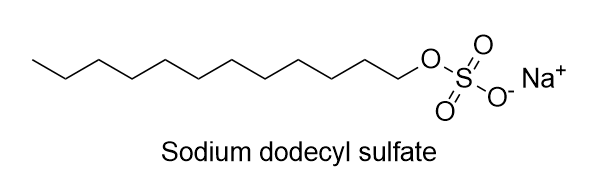
\includegraphics[width = 0.5\textwidth]{figure/Some Pictures/SDS.png}
    \caption{SDS的结构}
    \label{fig:enter-label}
\end{figure}

在$\beta$-巯基乙醇或二硫苏糖醇(DTT)的协助下,SDS能够彻底破坏蛋白质原有空间结构,形成特殊的棒状胶束螺旋型复合物,短轴大约$1.8\mathrm{nm}$ ;平均每两个氨基酸残基结合一个SDS分子;SDS疏水基插入在蛋白螺旋间隙,阴离子裸露朝外。
在沸水浴下,蛋白质与SDS的重量结合比大约为1.41。因此,蛋白质-SDS复合物上带上了大量的负电荷,完全掩盖了各种蛋白质分子本身原来的电荷差异,荷质比基本相同,但由于它们原本的分子量不同,所以棒状胶束的长轴具有差异,在通过聚丙烯酰胺凝胶网络时因分子筛效应而被分离。

\begin{figure}[H]
    \centering
    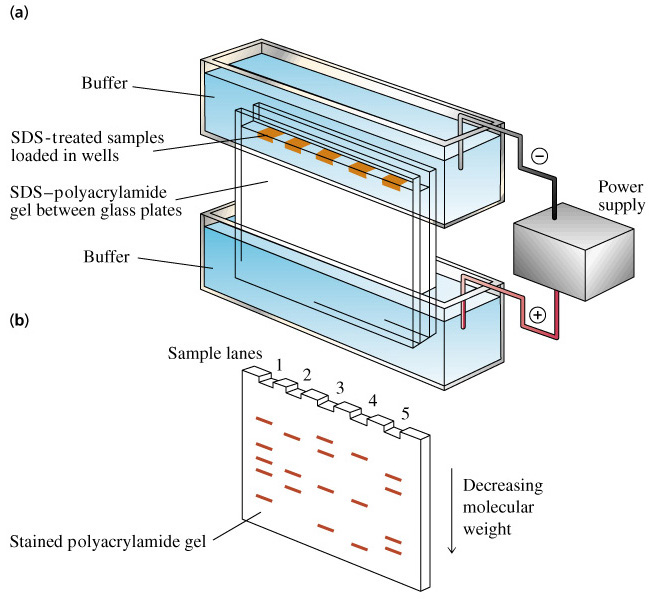
\includegraphics[width = 0.5\textwidth]{figure/Some Pictures/SDS-PAGE简图.png}
    \caption{SDS-Page示意图}
    \label{fig:enter-label}
\end{figure}

SDS-Page(sodium dodecyl sulfate-polyacrylamide gel electrophoresis)中存在三大效应:提供泳动力的电荷效应、压缩谱带宽幅并提高分辨效果的浓缩效应、决定分离效率和决定分辨率的分子筛效应。其中,浓缩效应来自于凝胶层的不连续性、缓冲液离子对的不连续性和缓冲液PH值的不连续性。

多数蛋白质分子量的常用对数值与其SDS-PAGE中的相对迁移率近似呈线性负相关,据此建立标曲,即可测定未知蛋白的分子量。
\begin{figure}[H]
    \centering
    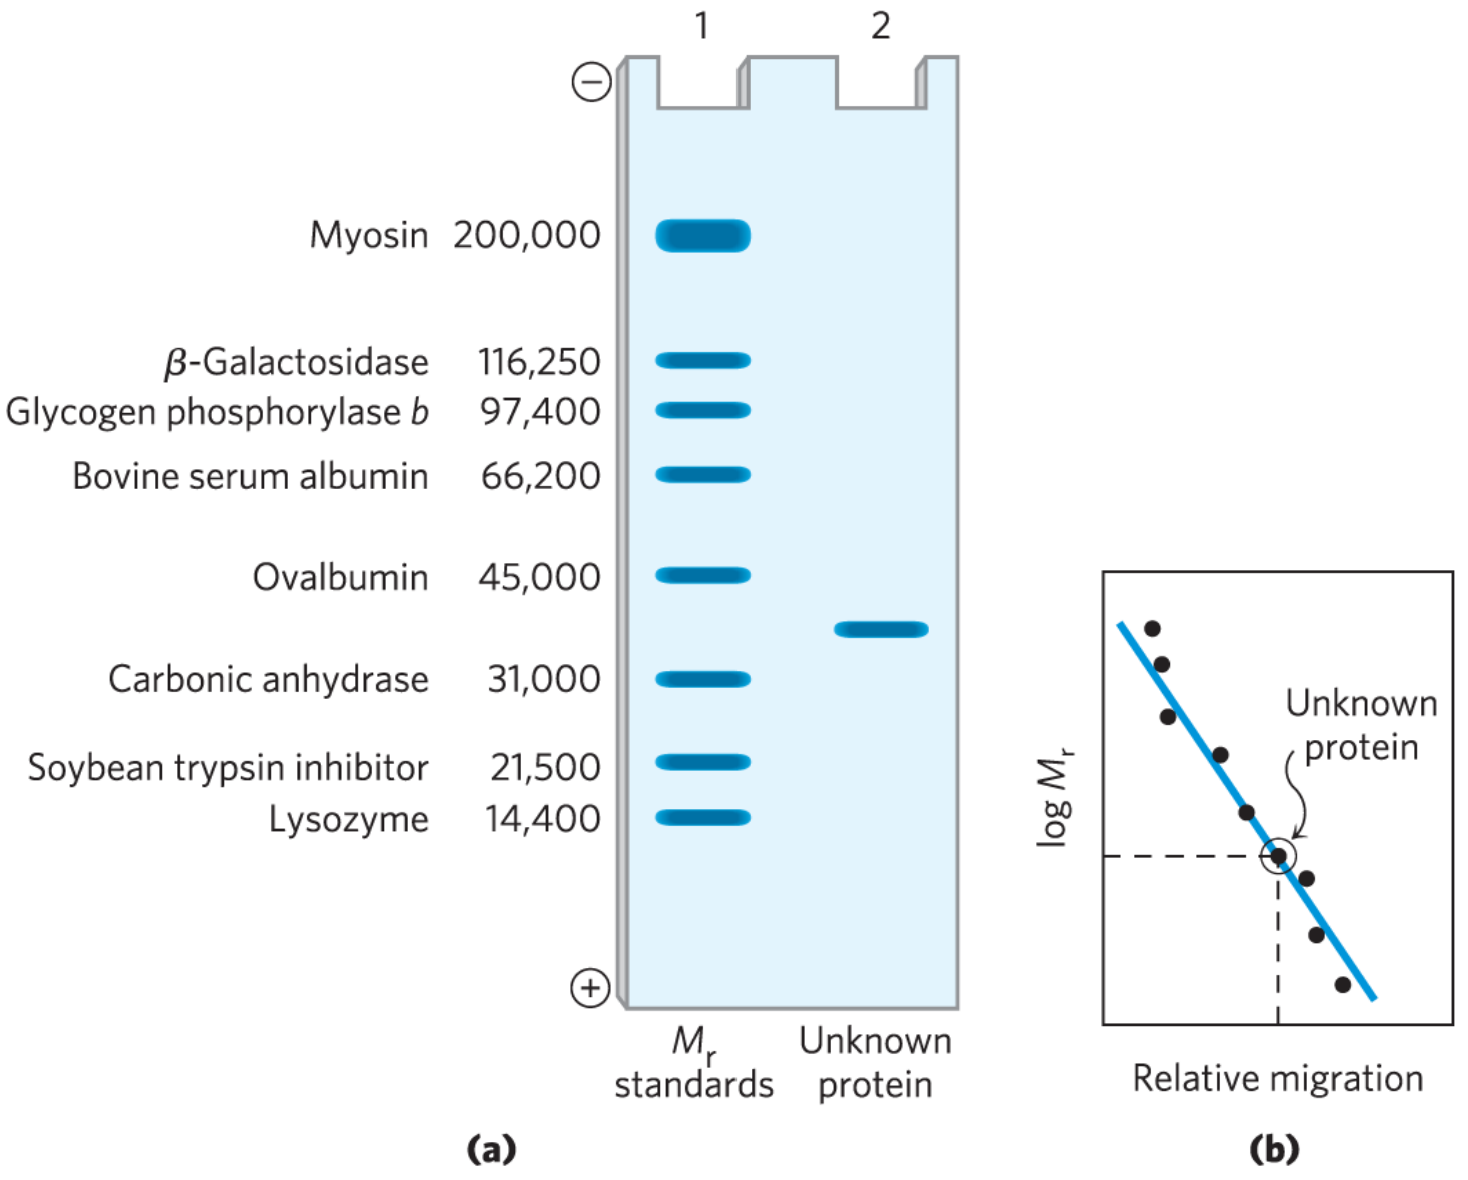
\includegraphics[width = 0.5\textwidth]{figure/Some Pictures/Estimating the molecular weight of a protein.png}
    \caption{估算蛋白质的分子量\cite{nelson2021lehninger}}
    \label{fig:enter-label}
\end{figure}

\subsubsection{糖蛋白电泳}
鉴定糖链的常用方法有很多。首先,样品可以经聚丙烯酰胺凝胶电泳后进行定性鉴定,使用高碘酸-Schiff法(形成较浅的红色或粉红色条带)、阿尔新蓝(Alcian blue)或甲苯胺蓝(Toluidine blue)等阳离子染料染色法、硫酸一百里苯酚染色法、Western印迹法(将蛋白条带转移至硝酸纤维素膜上,再以糖蛋白测定试剂盒进行染色)等方法进行染色。其次,可以使用凝集素法进行鉴定。凝集素能特异性识别和结合特异单糖或糖链结构,区别糖残基的连接方式、分支和修饰情况,可结合酶联免疫 (ELISA) 、印迹等方法鉴定分离糖链、糖肽及鉴定糖链结构。

蔗糖外酶是一种糖蛋白,有大约$50\%$的糖基化,本实验经电泳分离后对其进行糖蛋白定性,用希夫试剂进行显色观察。高碘酸希夫染色法一般用来鉴定糖元和其它多糖物质。高碘酸(多采用$\mathrm{pH}=3\sim5$)将多糖乙二醇基氧化成二醛,再与Schiff氏液的无色品红结合。需要注意的是,高碘酸是强氧化剂,它能破坏各种结构的C—C键,与乙二醇相似的氨基、烷基氨基衍生物或多糖分子的去氢葡萄糖残基均可被氧化产生醛基,此后醛基再与 Schiff 试剂结合产生紫红色。由于高碘酸可氧化其他物质,故氧化时间应控制好,不宜过久。

\subsubsection{活性蛋白电泳}
非变性聚丙烯酰胺凝胶电泳称为活性电泳(Native-PAGE),是指在不加入SDS和巯基乙醇等变性剂的条件下,对保持活性的蛋白质进行聚丙烯酰胺凝胶电泳。Native-PAGE和SDS-PAGE在操作上基本上相同,只是Native-PAGE凝胶的配制和电泳缓冲液中含有变性剂等。而像蔗糖酶这样经过SDS-PAGE操作后可通过添加复性剂恢复活性的蛋白也可使用SDS-PAGE的相关步骤加之相应的处理进行活性染色。

活性显色基本原理是先将蔗糖酶样品进行SDS-PAGE分离,取出凝胶后加入蔗糖底物保温反应,生产葡萄糖与果糖。在强碱性溶液中,加入四氮唑盐进行染色反应,还原生成有色甲臜显色。氯化三苯四氮唑还原
生成深红色的三苯甲臜,在$480\sim490\mathrm{nm}$波长处有最大吸收峰;蓝四氯唑还原生成暗蓝色的双甲臜,在525nm波长处有最大吸收。该反应在一定条件下可定量完成,且生成的有色甲臜具有一定的稳定性。

\subsubsection{Western Blot}
印迹法是指将样品电泳分离后转移到固相载体上,经分子杂交结合特异性分子标记,然后利用相应的探测技术(如放射自显影术、荧光显影术、酶标法、分光光度法等)来检测样品的一种方法。1975 年,Southern建立了将DNA转移到硝酸纤维素膜(NC膜)上并利用DNA-RNA杂交检测特定的DNA片段的方法,称为Southern印迹法。此后人们用类似的方法对RNA和蛋白质进行印迹分析。我们把对RNA的印迹分析称为Northern Blot,把对单向电泳后的蛋白质分子的印迹分析称为Western Blot,把对双向电泳后蛋白质分子的印迹分析称为Eastern Blot。

Western Blot是在蛋白质凝胶电泳和固相免疫测定基础上发展起来的蛋白质检测技术。首先,蛋白质样品先经过SDS-PAGE分离;然后,经电转移到固相载体(如硝酸纤维素薄膜)上,固相载体以非共价键形式吸附蛋白质,且能保持电泳分离的多肽类型及其生物学活性不变;接着,以固相载体上的蛋白质或多肽作为抗原,与对应的一抗抗体起免疫反应,然后酶或同位素标记的二抗抗体与一抗免疫结合;最后,经过底物显色、荧光、化学发光或放射自显影等,检测电泳分离的特异性目的基因表达的蛋白成分。Western Blot的灵敏度很高,常用于目的基因表达产物的鉴别和定性定量检测细胞中某个蛋白质的表达水平。

\begin{figure}[H]
    \centering
    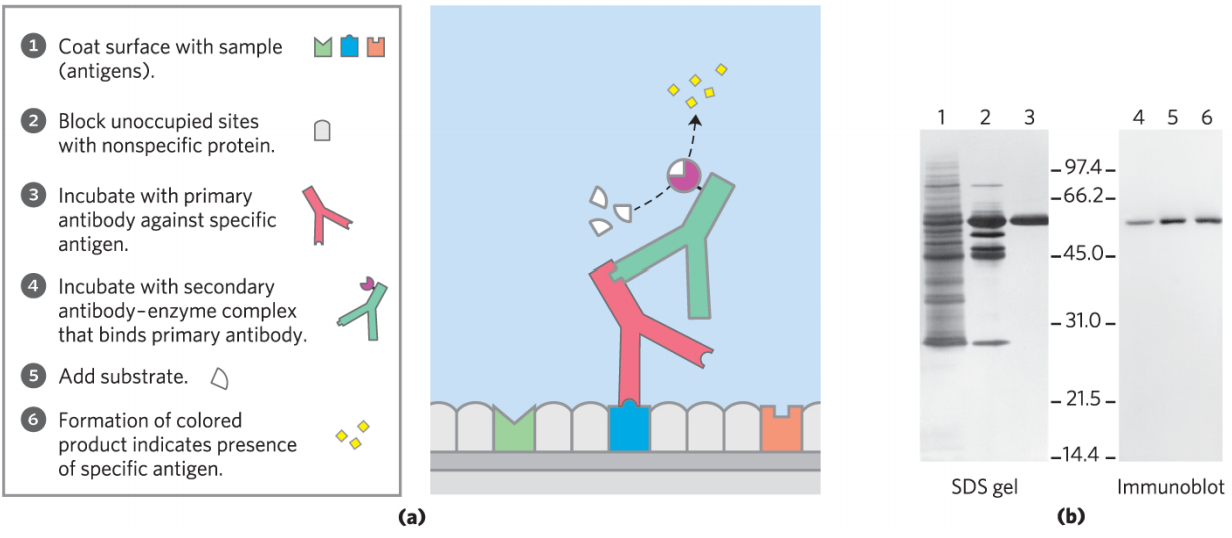
\includegraphics[width = 0.7\textwidth]{figure/Some Pictures/Antibodies as analytical reagents.png}
    \caption{抗体在Western Blot中作为分析试剂~\cite{nelson2021lehninger}}
    \label{fig:enter-label}
\end{figure}

\subsubsection{酶促反应动力学}
\par $K_\mathrm{m}$是酶的一个特征性常数,对一定底物、一定的pH和温度是常量。可以用于鉴定酶种类、判断反应趋势及抑制类型等。$V_\text{max}$是酶被底物饱和时的反应速率,对特定底物、特定条件是常数。米氏方程揭示了单底物酶促反应初速率与底物浓度之间的定量关系,如\autoref{eq:Muller}所示。
\begin{equation}
    V_0 = \frac{V_\text{max}[S]}{K_\text{m} + [S]}
    \label{eq:Muller}
\end{equation}
为了更好得到线性关系,可将\autoref{eq:Muller}取导数,得Lineweaver-Burk双倒数曲线:
\begin{equation}
    \frac{1}{V_0} = \frac{K_\text{m}}{V_\text{max}}\,\frac{1}{[S]} + \frac{1}{V_\text{max}}
    \label{eq:Lineweaver-Burk}
\end{equation}
\par 本实验中控制不同蔗糖浓度下进行反应,通过DNS显色、分光光度测量,计算对应的$1/[S]$和$1/V_0$,根据\autoref{eq:Lineweaver-Burk}作Lineweaver-Burk双倒数曲线,可以求得该酶促反应的动力学参数$K_\text{m}$值和$V_\text{max}$,并且用同样方法可探究变性剂尿素浓度对蔗糖酶活性的影响。

\section{实验步骤}

\subsection{蔗糖酶的分离与纯化}
\subsubsection{破壁粗提}
12g干酵母加适量石英砂于研钵中研磨,直至成细粉末,加入40mL20mmol/L Tris-Cl pH=7.4 缓冲液,继续研磨10分钟,至成为糊状液体,均匀分装到两支50mL离心管中,4\dc 15000rpm 离心20分钟,滴管收集中间水层溶液,得样品$\mathrm{I}$,量筒读数记录体积,留样备用,剩余样品分装到离心管中备用。
\subsubsection{热处理}
50\dc 热水浴保温30分钟,冰水浴冷却至室温,4\dc  12000rpm 离心15分钟,倾倒收集上清液,得样品$\mathrm{II}$中,记录体积,留样,剩余样品转移到250mL烧杯中冰浴备用。
\subsubsection{乙醇沉淀和复性溶解}
量取等体积-20\dc 的95\%乙醇,快速倾倒入烧杯混匀,冰浴静置20分钟,均匀转移至离心管中,4\dc ,12000rpm 离心10分钟,弃去上清,向各沉淀物离心管中加入15mL20mmol/L Tris-Cl pH=7.4 缓冲液,吹打混匀,复性溶解,4\dc  12000rpm 离心10分钟,留取上清液,得样品$\mathrm{III}$中,记录体积,留样备用,剩余样品继续离子交换色谱。
\subsubsection{阴离子交换色谱纯化蛋白}

\begin{enumerate}
\item \textbf{装柱与平衡}
\par 色谱柱垂直放置,两端接入主机;吸取3mL上清加入层析柱中;摇匀后将填料加入柱中;观察分界面到达15cm高度后停止加入填料;上方加3cm缓冲液A;
\item  \textbf{上样}
   \par 关闭恒流泵阀,停止平衡洗脱;滴管吸取树脂上端缓冲液A,至凹液面相切;沿柱壁用滴管缓慢加入样品3,直至全部加完;打开恒流泵阀,使样品完全进入树脂;
\item \textbf{穿流洗脱}
    \par 关闭恒流泵,加入2cm高度的缓冲液A ;连接色谱柱上端到A瓶,系统完全密封;
    \par 打开泵阀,连续洗脱,去除未结合杂质;;直至穿流峰完全回落,记录仪曲线回到基线位置;
\item \textbf{梯度洗脱}
 \par 设置盐度梯度,部分收集2mL/管;至吸收峰回落停止收集。
\end{enumerate}

\subsubsection{蔗糖酶活性检测}

配置预混液(0.1mol/L pH=4.6乙酸缓冲液,5\%蔗糖溶液,去离子水==1:1:2);除空白对照组外,每管依次加5 µL样品,涡旋混匀;50\dc 水浴10分钟;加入0.5mLDNS,涡旋混匀;100\dc 水浴5分钟,冷却至室温;加5.0mL去离子水,混匀观察比色。

\subsection{纯化方案评价}
\subsubsection{蛋白质标准曲线的制作}
根据\autoref{tab:stdcurve_protein}进行实验,计算相应的蛋白质浓度,并将其对$\lambda = 650$nm下测得吸光度绘图,得到蛋白质标准曲线。

\begin{table}[H]
\centering
\caption{蛋白质浓度标准曲线的绘制}
\label{tab:stdcurve_protein}
\begin{tabular}{@{}ccccccc@{}}
\toprule
\diagbox[height = 3em]{试剂}{试管号} & 1   & 2   & 3   & 4   & 5   & 6   \\ \midrule
牛血清白蛋白含量/mg           & 0   & 0.1 & 0.2 & 0.3 & 0.4 & 0.5 \\
0.5g/L牛血清白蛋白溶液/mL     & 0   & 0.2 & 0.4 & 0.6 & 0.8 & 1   \\
去离子水/mL               & 1   & 0.8 & 0.6 & 0.4 & 0.2 & 0   \\
样品体系总体积/mL            & 1   & 1   & 1   & 1   & 1   & 1   \\
Folin-酚试剂甲/mL         & 5   & 5   & 5   & 5   & 5   & 5   \\ \midrule
\multicolumn{7}{c}{\textbf{涡旋仪混匀,25\dc 水浴10 min}}                     \\ \midrule
Folin-酚试剂乙/mL         & 0.5 & 0.5 & 0.5 & 0.5 & 0.5 & 0.5 \\\midrule
\multicolumn{7}{c}{\textbf{即刻涡旋仪混匀,25\dc 水浴15min,比色检测}}              \\ \bottomrule
\end{tabular}
\end{table}

\subsubsection{各样品蛋白质含量的测定}
首先根据\autoref{tab:protein_op_pre_tabel}对样品IV不同样品用量进行预实验(操作同\autoref{tab:stdcurve_protein}),选择分光度在0.7-0.9的条件,再根据\autoref{tab:protein_op_table}对四份样本进行蛋白质浓度测定。

\begin{table}[H]
\centering
\caption{测定各样本蛋白质含量预实验操作表}
\label{tab:protein_op_pre_tabel}
\begin{tabular}{@{}cccc@{}}
\toprule
              & 1    & 2   & 3   \\ \midrule
样品IV溶液/mL     & 0.05 & 0.1 & 0.3 \\
去离子水/mL       & 0.95 & 0.9 & 0.7 \\
总体积/mL        & 1    & 1   & 1   \\
Folin-酚甲试剂/mL & 5    & 5   & 5   \\
Folin-酚乙试剂/mL & 0.5  & 0.5 & 0.5 \\ \bottomrule
\end{tabular}
\end{table}

\begin{table}[H]
\centering
\caption{测定各样本蛋白质含量操作表}
\label{tab:protein_op_table}
\begin{tabular}{@{}ccccc@{}}
\toprule
样品编号          & 样品$\mathrm{I}$ $\times$20稀释 & 样品$\mathrm{II}$ $\times$15稀释 & 样品$\mathrm{III}$ $\times$10稀释 & 样品$\mathrm{IV}$ \\ \midrule
样品溶液/mL        & 0.15     & 0.15     & 0.15      & 0.15 \\
去离子水/mL        & 0.85     & 0.85     & 0.85      & 0.85 \\
总体积/mL         & 1        & 1        & 1         & 1    \\
Folin-酚甲试剂/mL  & 5        & 5        & 5         & 5    \\ 
Folin-酚乙试剂/mL     & 0.5      & 0.5      & 0.5       & 0.5  \\  \bottomrule
\end{tabular}
\end{table}

\subsubsection{蛋白洗脱曲线的测定}
按照\autoref{tab:protein_curve_op}配置各试管溶液,测定其吸光度,并计算各样品蛋白含量。

\begin{table}[H]
\centering
\caption{蛋白洗脱曲线的测定}
\label{tab:protein_curve_op}
\resizebox{\textwidth}{!}{%
\begin{tabular}{@{}ccccccccccccccc@{}}
\toprule
试管编号          & \multicolumn{1}{l}{空白}  & 穿流   & 14   & 15   & 16   & 17   & 18   & 19   & 20   & 21   & 22   & 23   & 24   & 25   \\ \midrule
样品IV溶液/mL     & 0                       & 0.15 & 0.15 & 0.15 & 0.15 & 0.15 & 0.15 & 0.15 & 0.15 & 0.15 & 0.15 & 0.15 & 0.15 & 0.15 \\
去离子水/mL       & 1                       & 0.85 & 0.85 & 0.85 & 0.85 & 0.85 & 0.85 & 0.85 & 0.85 & 0.85 & 0.85 & 0.85 & 0.85 & 0.85 \\
总体积/mL        & 1                       & 1    & 1    & 1    & 1    & 1    & 1    & 1    & 1    & 1    & 1    & 1    & 1    & 1    \\
Folin-酚甲试剂/mL & 5                       & 5    & 5    & 5    & 5    & 5    & 5    & 5    & 5    & 5    & 5    & 5    & 5    & 5    \\
Folin-酚乙试剂/mL & \multicolumn{1}{l}{0.5} & 0.5  & 0.5  & 0.5  & 0.5  & 0.5  & 0.5  & 0.5  & 0.5  & 0.5  & 0.5  & 0.5  & 0.5  & 0.5  \\ \bottomrule
\end{tabular}%
}
\end{table}

\subsubsection{葡萄糖标准曲线的制作}

根据\autoref{tab:stdcurve_glucose}进行实验,计算相应的蛋白质浓度,并将其对$\lambda = 520$nm下测得吸光度绘图,得到蛋白质标准曲线。

\begin{table}[H]
\centering
\caption{葡萄糖浓度标准曲线的绘制}
\label{tab:stdcurve_glucose}
\begin{tabular}{@{}ccccccc@{}}
\toprule
\diagbox[height = 3em]{试剂}{试管号}     & 0     & 1     & 2    & 3    & 4    & 5    \\ \midrule
葡萄糖含量/mg             & 0     & 0.1   & 0.2  & 0.3  & 0.4  & 0.5  \\
1g/L葡萄糖标准溶液/mL       & 0     & 0.1   & 0.2  & 0.3  & 0.4  & 0.5  \\
去离子水/mL              & 2.0     & 1.9   & 1.8  & 1.7  & 1.6  & 1.5  \\
反应体系总体积/mL           & 2     & 2     & 2    & 2    & 2    & 2    \\
3.5-二硝基水杨酸(DNS)/mL   & 0.5   & 0.5   & 0.5  & 0.5  & 0.5  & 0.5  \\ \midrule
\multicolumn{7}{c}{\textbf{涡旋仪混匀,$>$95\dc 水浴5min,冷却至室温}} \\ \midrule
去离子水/mL              & 5     & 5     & 5    & 5    & 5    & 5    \\ \bottomrule
\end{tabular}
\end{table}

\subsubsection{各样品活性的测定}
首先根据\autoref{tab:glucose_pre_op_table}对样品IV不同样品用量进行预实验(操作同\autoref{tab:stdcurve_glucose}),选择分光度在0.7-0.9的条件,再根据\autoref{tab:glucose_op_table}对四份样本进行蛋白质浓度测定。

\begin{table}[H]
\centering
\caption{测定各样本蔗糖酶活性}
\label{tab:glucose_pre_op_table}
\begin{tabular}{@{}cccc@{}}
\toprule
试管号          & 1    & 2    & 3    \\ \midrule
0.1M乙酸缓冲液/mL & 0.5  & 0.5  & 0.5  \\
去离子水/mL      & 0.99 & 0.98 & 0.95 \\
蔗糖酶液/mL      & 0.01 & 0.02 & 0.05 \\
5%蔗糖溶液/mL    & 0.5  & 0.5  & 0.5  \\
反应总体积/mL     & 2    & 2    & 2    \\
DNS试剂/mL     & 0.5  & 0.5  & 0.5  \\
去离子水/mL      & 5    & 5    & 5    \\ \bottomrule
\end{tabular}
\end{table}

\begin{table}[H]
\centering
\caption{测定各样本蔗糖酶活性}
\label{tab:glucose_op_table}
\resizebox{\textwidth}{!}{%
\begin{tabular}{@{}ccccc@{}}
\toprule
样品           & 样品I$\times$2000稀释 & 样品II$\times$2000稀释 & 样品III$\times$1000稀释 & 样品IV$\times$500稀释 \\ \midrule
0.1M乙酸缓冲液/mL & 0.5         & 0.5          & 0.5        & 0.5        \\
去离子水/mL      & 0.95        & 0.95         & 0.95       & 0.95       \\
蔗糖酶液/mL      & 0.037       & 0.037        & 0.037      & 0.037      \\
5\%蔗糖溶液/mL    & 0.5         & 0.5          & 0.5        & 0.5        \\
反应总体积/mL     & 2           & 2            & 2          & 2          \\
DNS试剂/mL     & 0.5         & 0.5          & 0.5        & 0.5        \\
去离子水/mL      & 5           & 5            & 5          & 5          \\ \bottomrule
\end{tabular}
}
\end{table}

\subsubsection{活性洗脱曲线的测定}
按照\autoref{tab:glucose_curve_op_table}配置各试管溶液,测定其吸光度,并计算各样品蔗糖酶活性。

\begin{table}[H]
\centering
\caption{测定各样本蔗糖酶活性}
\label{tab:glucose_curve_op_table}
\resizebox{\textwidth}{!}{%
\begin{tabular}{@{}ccccccccccccccc@{}}
\toprule
试管标号         & 空白  & 穿流    & 14    & 15    & 16    & 17    & 18    & 19    & 20    & 21    & 22    & 23    & 24    & 25    \\ \midrule
0.1M乙酸缓冲液/mL & 0.5 & 0.5   & 0.5   & 0.5   & 0.5   & 0.5   & 0.5   & 0.5   & 0.5   & 0.5   & 0.5   & 0.5   & 0.5   & 0.5   \\
去离子水/mL      & 1   & 0.963 & 0.963 & 0.963 & 0.963 & 0.963 & 0.963 & 0.963 & 0.963 & 0.963 & 0.963 & 0.963 & 0.963 & 0.963 \\
蔗糖酶液/mL      & 0   & 0.037 & 0.037 & 0.037 & 0.037 & 0.037 & 0.037 & 0.037 & 0.037 & 0.037 & 0.037 & 0.037 & 0.037 & 0.037 \\
5%蔗糖溶液/mL    & 0.5 & 0.5   & 0.5   & 0.5   & 0.5   & 0.5   & 0.5   & 0.5   & 0.5   & 0.5   & 0.5   & 0.5   & 0.5   & 0.5   \\
反应总体积/mL     & 2   & 2     & 2     & 2     & 2     & 2     & 2     & 2     & 2     & 2     & 2     & 2     & 2     & 2     \\
DNS试剂/mL     & 0.5 & 0.5   & 0.5   & 0.5   & 0.5   & 0.5   & 0.5   & 0.5   & 0.5   & 0.5   & 0.5   & 0.5   & 0.5   & 0.5   \\
去离子水/mL      & 5   & 5     & 5     & 5     & 5     & 5     & 5     & 5     & 5     & 5     & 5     & 5     & 5     & 5     \\ \bottomrule
\end{tabular}
}
\end{table}

\subsection{蔗糖酶酶切去糖基化}


\subsection{正交试验探究最佳反应条件}
\begin{enumerate}
    \item 制作因素-水平表
    \par \hspace*{2em} 四个基本因素:底物浓度$[S]$、酶浓度$[E]$、温度$T$、$\mathrm{pH}$值,每个因素设置三个水平,各因素的水平值排列顺序,要求不能有明显的数学逻辑关系(等差、等比、全降序、全升序)。不考虑交互作用,可以任意决定把哪一个因素排在哪一列。
    \par \hspace*{2em} 由于实验条件的限制,温度和pH值固定了3个水平值,但可以调整排列的顺序。[S]和[E]的水平值和排列完全自主决定。一旦表头排定,试验方案就确定了,不可中途更改。
    
\begin{table}[H]
\centering
\caption{正交试验表头}
\label{tab:my-table}
\begin{tabular}{|c|p{4em}<{\centering}|p{4em}<{\centering}|p{4em}<{\centering}|p{4em}<{\centering}|}
\hline \diagbox{水平}{因素}
 & \begin{tabular}[c]{@{}c@{}}{[}S{]}\\ /mL\end{tabular} & \begin{tabular}[c]{@{}c@{}}{[}E{]}\\ /mL\end{tabular} & \begin{tabular}[c]{@{}c@{}}温度\\ /\dc \end{tabular} & pH值 \\ \hline
水平I   & 0 & 0 & 0 & 0 \\ \hline
水平II  & 1 & 1 & 1 & 1 \\ \hline
水平III & 2 & 2 & 2 & 2 \\ \hline
\end{tabular}
\end{table}

\begin{table}[H]
\centering
\caption{正交试验表头}
\label{tab:my-table}
\begin{tabular}{@{}cp{4em}<{\centering}p{4em}<{\centering}p{4em}<{\centering}p{4em}<{\centering}@{}}
\toprule
\diagbox{水平}{因素}      & {[}S{]} & {[}E{]} & T & pH \\ \midrule
水平I   & 0       & 0       & 0 & 0  \\
水平II  & 1       & 1       & 1 & 1  \\
水平III & 2       & 2       & 2 & 2  \\ \bottomrule
\end{tabular}
\end{table}

    \item 选择正交表,代入数值
    \par \hspace*{2em} 选择$L^{9}(3^{4})$正交表进行正交试验,把[S]、[E]、T和pH值四个因素分别填在正交表的A、B、C、D四列上方,称作排表头。把各水平数值按照表头中的排列填入正交表正确位置。

\begin{table}[H]
\centering
\caption{$L^{9}(3^{4})$正交表}
\label{tab:my-table}
\begin{tabular}{|c|p{4em}<{\centering}|p{4em}<{\centering}|p{4em}<{\centering}|p{4em}<{\centering}|}
\hline
\diagbox{实验号}{水平}{因素}  & A & B & C & D \\ \hline
1 & 0 & 0 & 0 & 0 \\ \hline
2 & 0 & 1 & 1 & 1 \\ \hline
3 & 0 & 2 & 2 & 2 \\ \hline
4 & 1 & 0 & 1 & 2 \\ \hline
5 & 1 & 1 & 2 & 0 \\ \hline
6 & 1 & 2 & 0 & 1 \\ \hline
7 & 2 & 0 & 2 & 1 \\ \hline
8 & 2 & 1 & 0 & 2 \\ \hline
9 & 2 & 2 & 1 & 0 \\ \hline
\end{tabular}
\end{table}

\item 根据正交表执行实验

\end{enumerate}

\subsection{SDS-PAGE}

\subsection{糖蛋白电泳}

\subsection{活性蛋白电泳}

\subsection{Western Blot}

\subsection{酶促反应动力学}



\section{实验数据处理和结果}

\subsection{蔗糖酶的分离与纯化}
 \par 如图所示,随着盐度梯度和离子电导率的移动,在23-60分钟出现一个紫外吸收峰,检测到洗脱出的待提取蛋白质,75-102分钟出现第二个紫外吸收峰,推测为较高盐度下废弃物峰。对收集得样品进行蔗糖酶活性检测,发现显色呈现先加深后变浅的变化,与紫外检测相符合。通过与空白组对照,第16-22号收集管有酶活力。
 
\subsection{蛋白质浓度测定}
实验得到蛋白质标准曲线相关数据如\autoref{tab:result_PROTEIN_STD}所示。根据操作\autoref{tab:stdcurve_protein}可知,各个试管中蛋白质的浓度计算公\autoref{eq:c_protein}

\begin{equation}
    c = \frac{m_\text{牛血清蛋白}}{V_\text{总体积}+V_\text{Folin-酚试剂甲}+V_\text{Folin-酚试剂乙}}
    \label{eq:c_protein}
\end{equation}

\begin{table}[H]
\centering
\caption{蛋白质标准曲线绘制实验结果}
\label{tab:result_PROTEIN_STD}
\begin{tabular}{@{}ccccccc@{}}
\toprule
试管号       & 1     & 2     & 3     & 4     & 5     & 6     \\ \midrule
牛血清白蛋白浓度/$10^{-2}\mathrm{g \cdot L^{-1}}$ & 0.000 & 1.538 & 3.077 & 4.615 & 6.154 & 7.692 \\
650nm下吸光度 & 0.000 & 0.277 & 0.506 & 0.670 & 0.852 & 0.938 \\ \bottomrule
\end{tabular}
\end{table}

绘制蛋白质浓度-650nm波长下吸光度,可得标准曲线如\autoref{fig:STD_Protein}所示。

\begin{figure}[H]
    \begin{minipage}[t]{0.48\textwidth}
        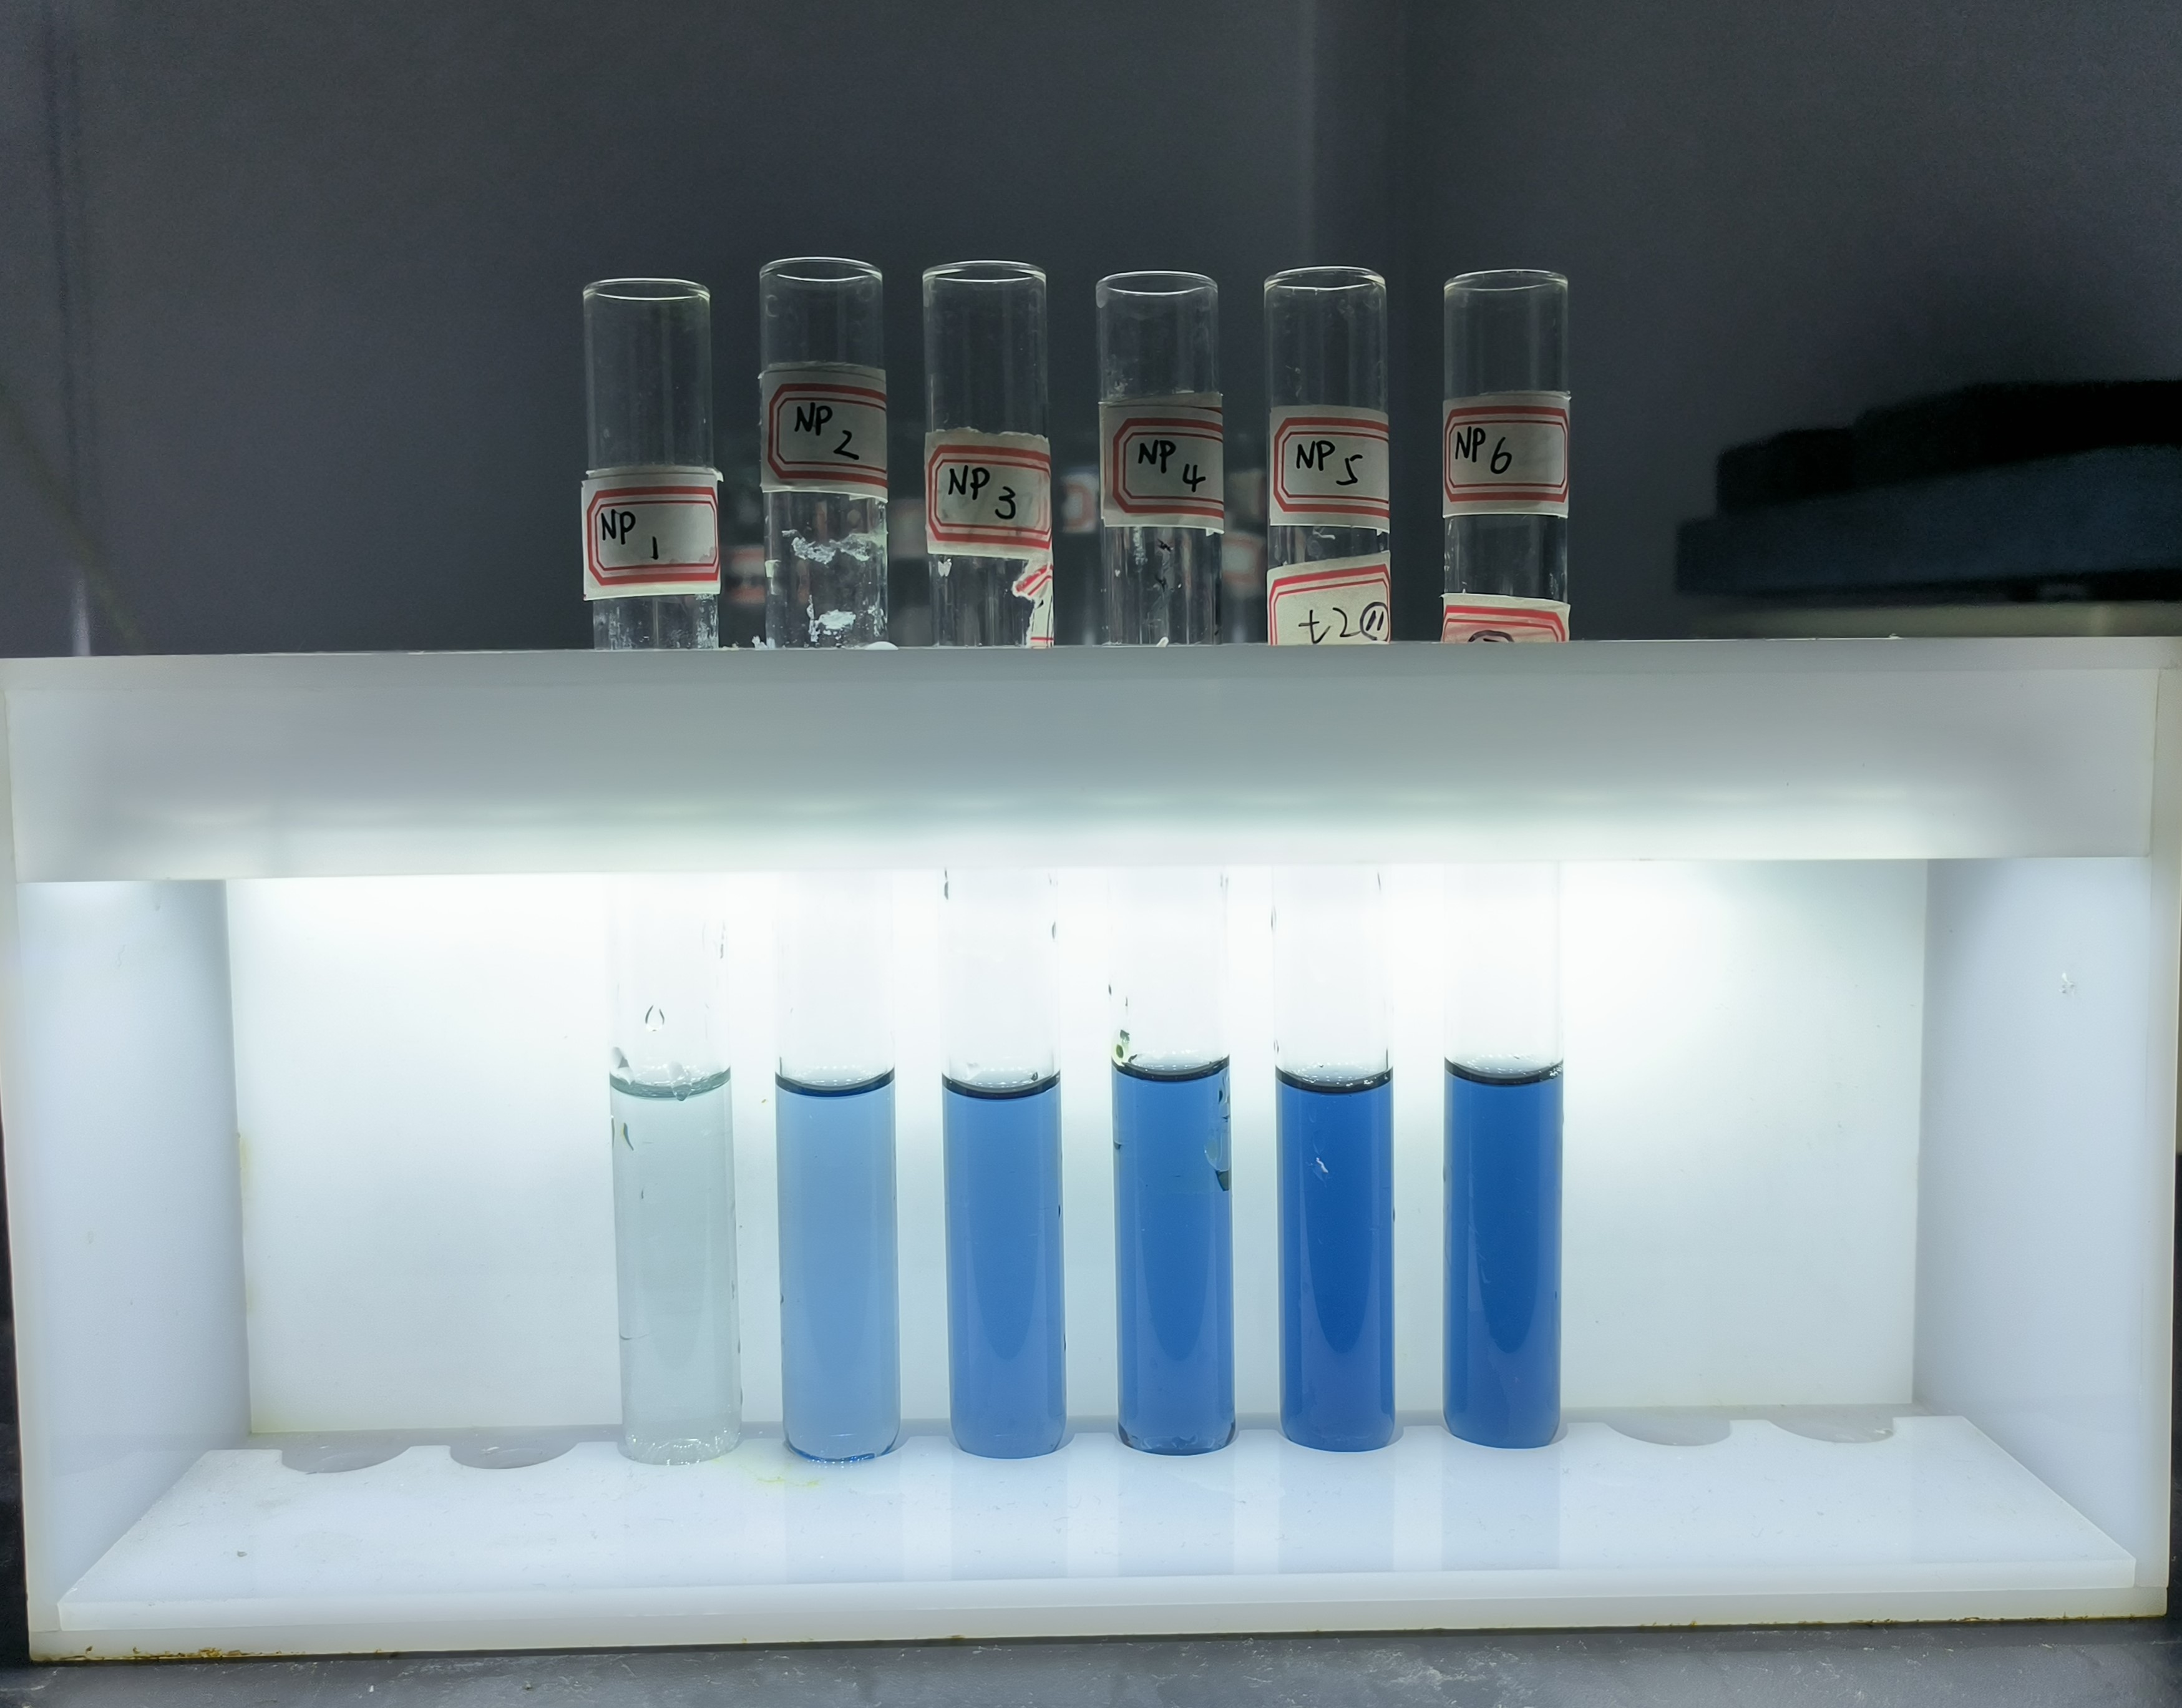
\includegraphics[width = \textwidth]{figure/1124/Pro_STD.jpg}
        \caption{蛋白质标准浓度实验结果图}
        \label{fig:STD_Protein_result}
    \end{minipage}
    % \centering
    \begin{minipage}[t]{0.50\textwidth}
        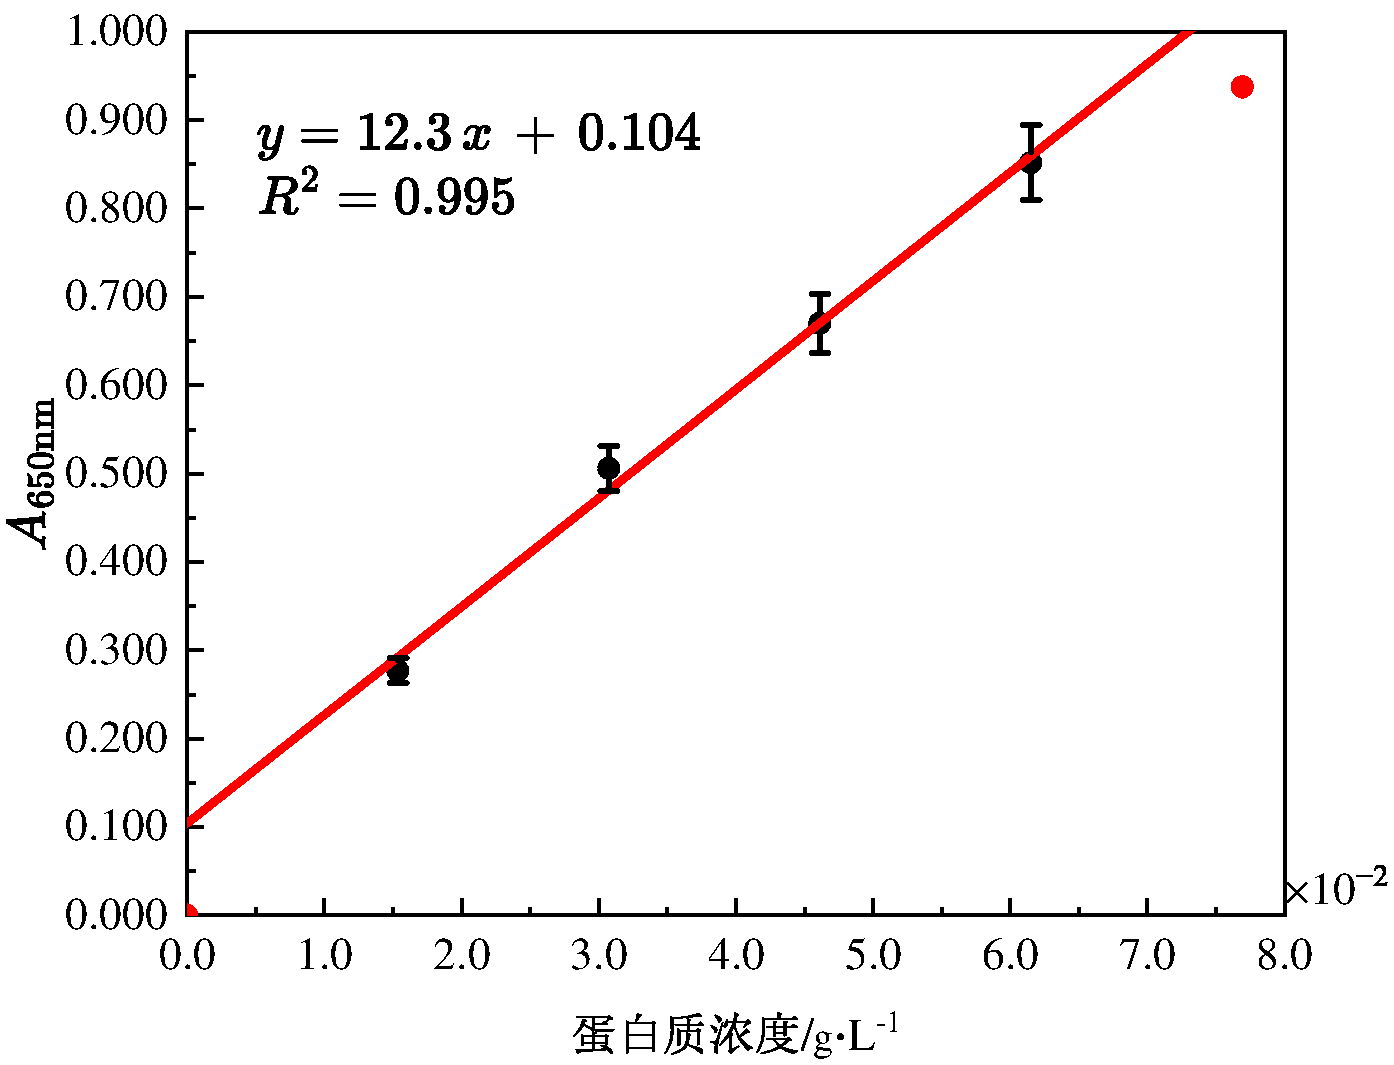
\includegraphics[width = \textwidth]{figure/1124/Protein_STD.pdf}
        \caption{蛋白质标准浓度曲线}
        \label{fig:STD_Protein}
    \end{minipage}
\end{figure}

根据所得的蛋白质标准曲线,对四个样本中的蛋白质含量进行测定,得

\begin{figure}[H]
    \begin{minipage}[t]{0.49\textwidth}
        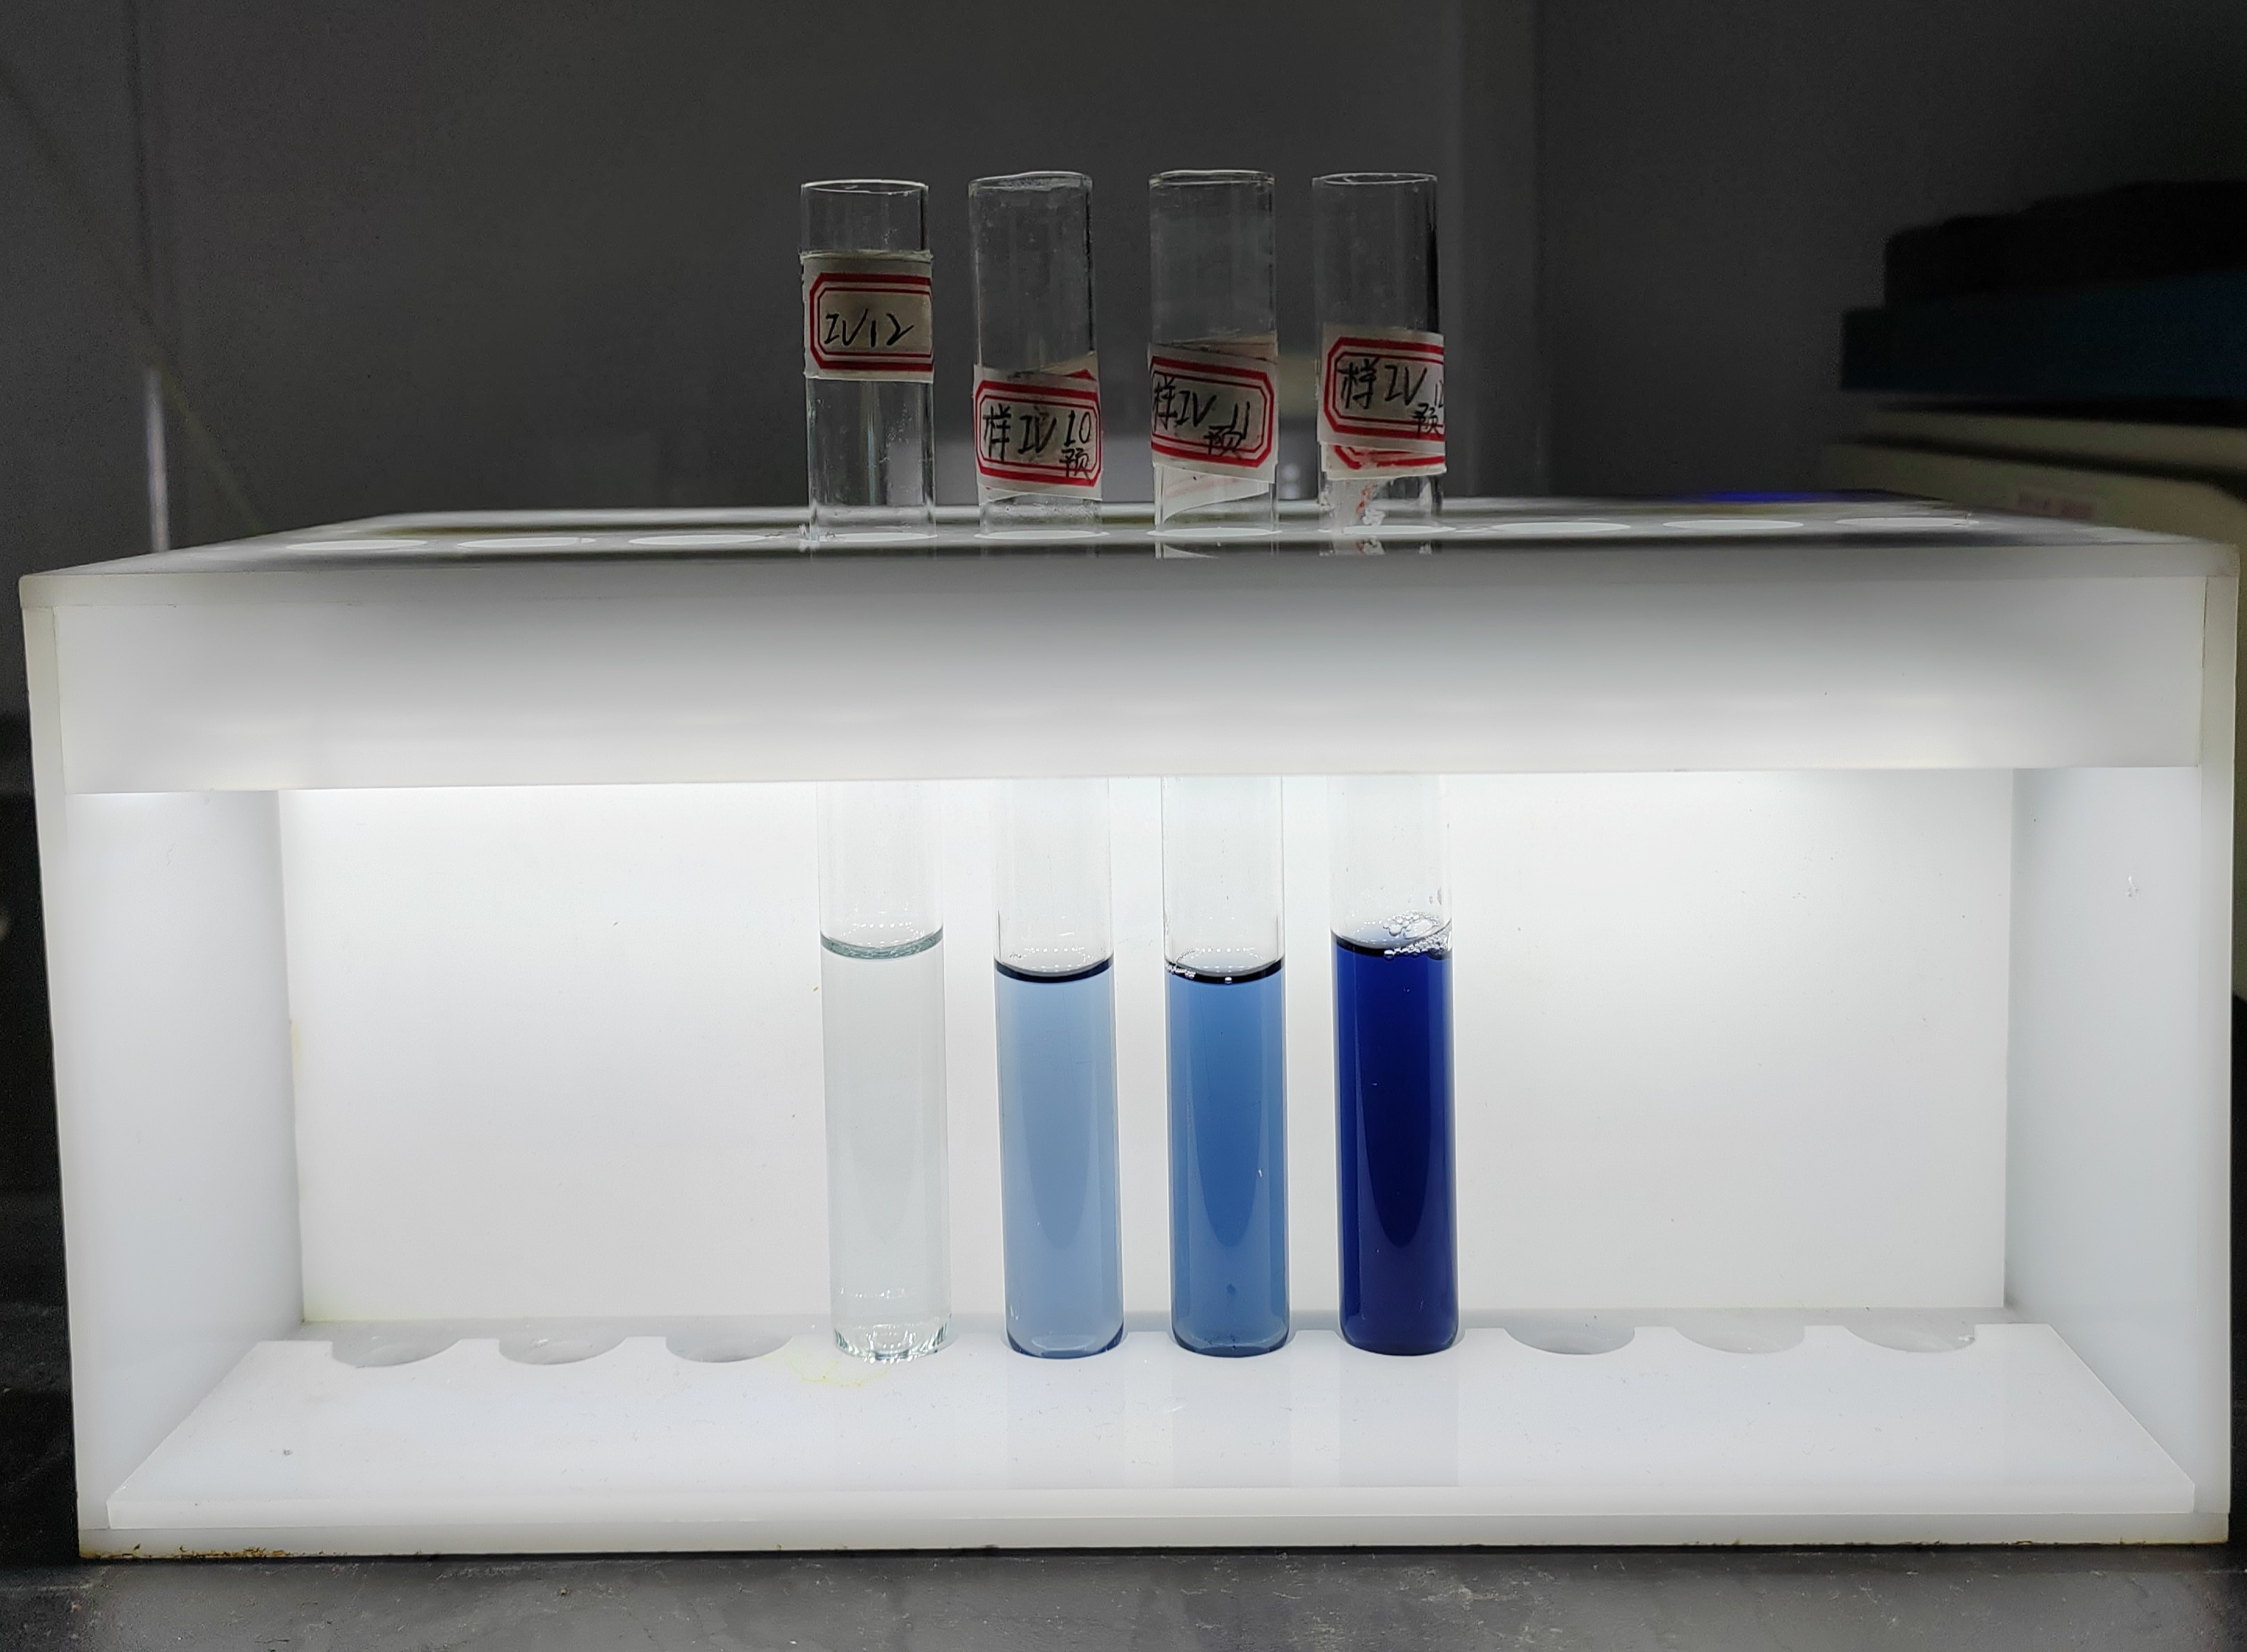
\includegraphics[width = \textwidth]{figure/1124/Pro_Samples.jpg}
        \caption{各样品蛋白质浓度测定实验结果图}
        \label{fig:Pro_Samples_result}
    \end{minipage}
    % \centering
    \begin{minipage}[t]{0.48\textwidth}
        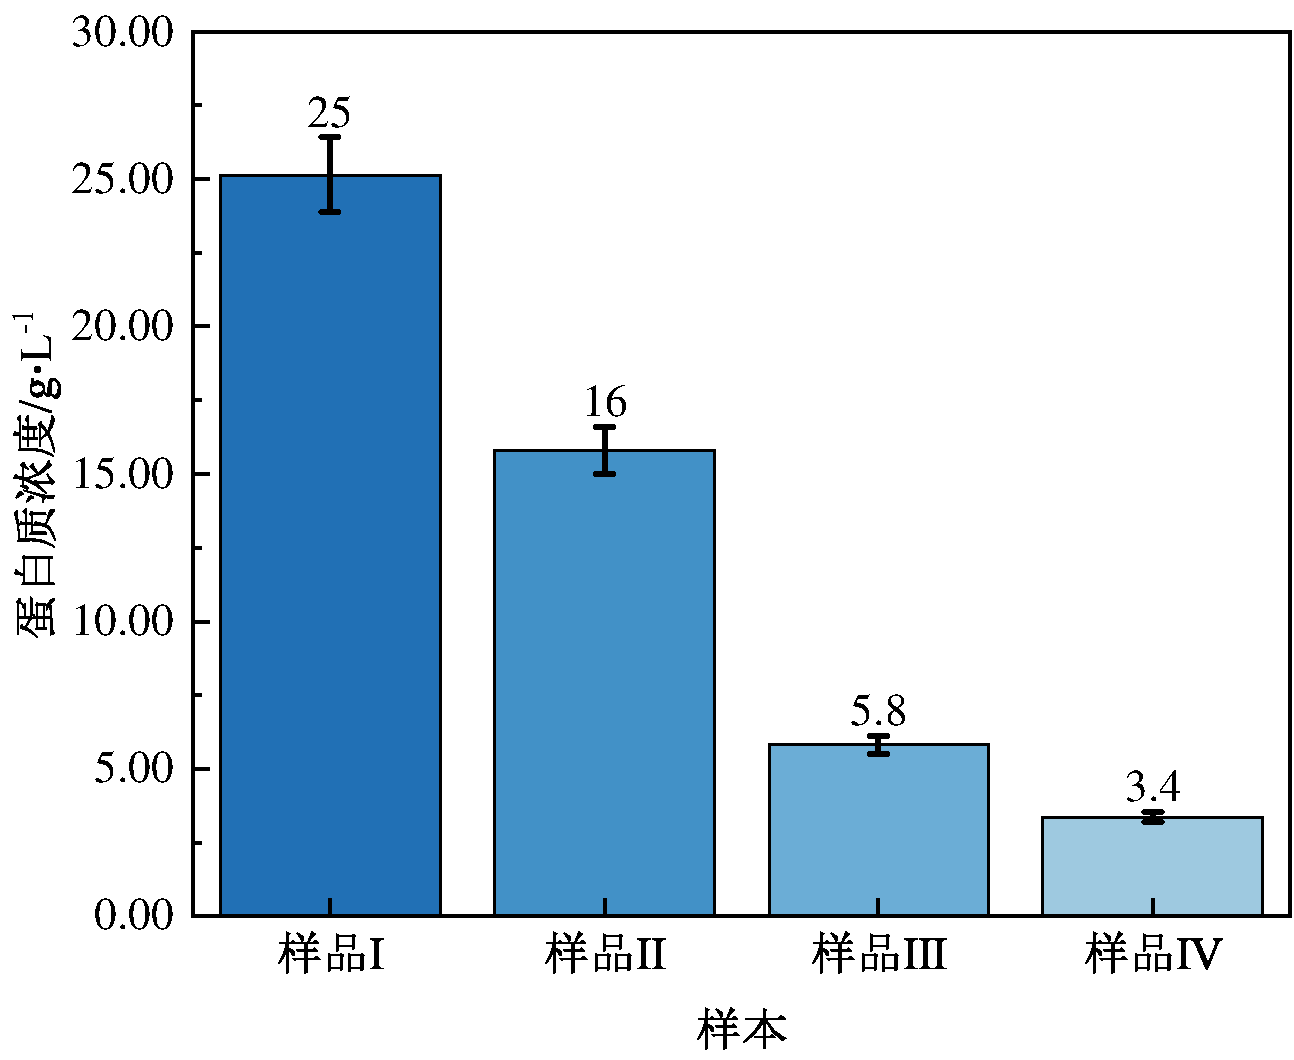
\includegraphics[width = \textwidth]{figure/1124/Protein_Samples.pdf}
        \caption{各样品蛋白质浓度}
        \label{fig:Pro_Samples}
    \end{minipage}
\end{figure}

\begin{figure}[H]
    \begin{minipage}[t]{0.47\textwidth}
        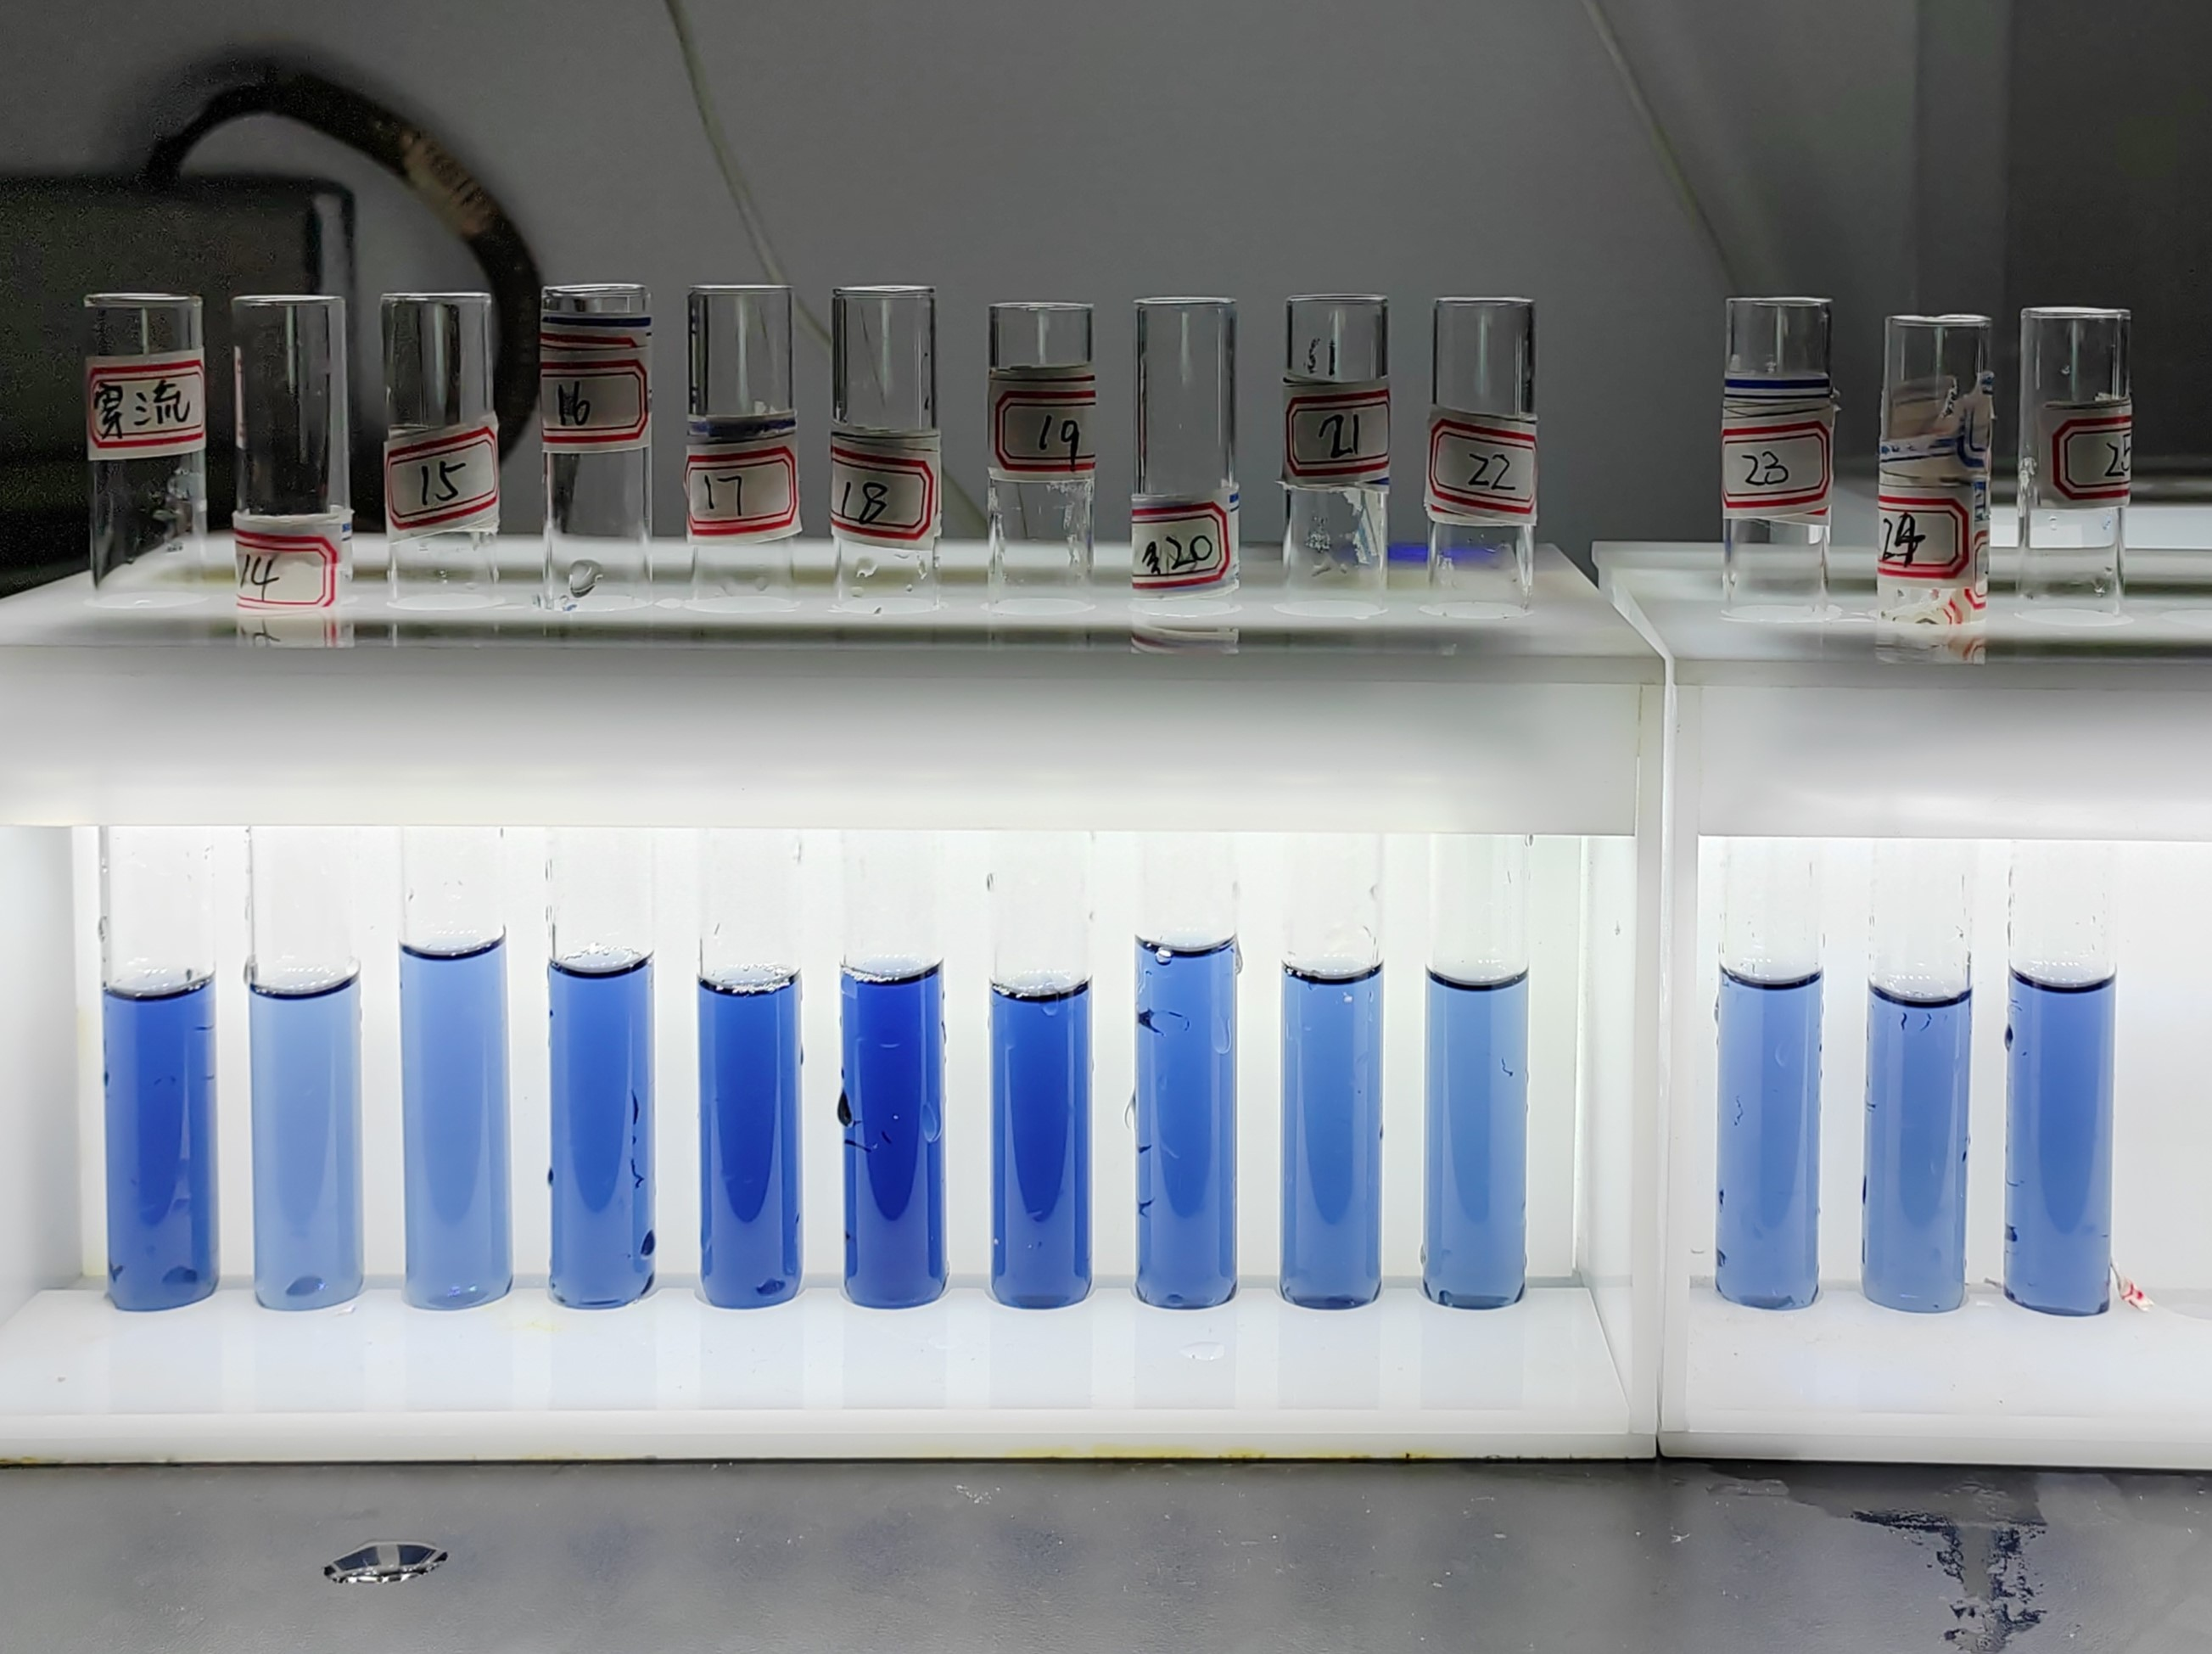
\includegraphics[width = \textwidth]{figure/1124/Pro_Curve.jpg}
        \caption{蛋白洗脱曲线实验结果图}
        \label{fig:Pro_Curve_result}
    \end{minipage}
    % \centering
    \begin{minipage}[t]{0.52\textwidth}
        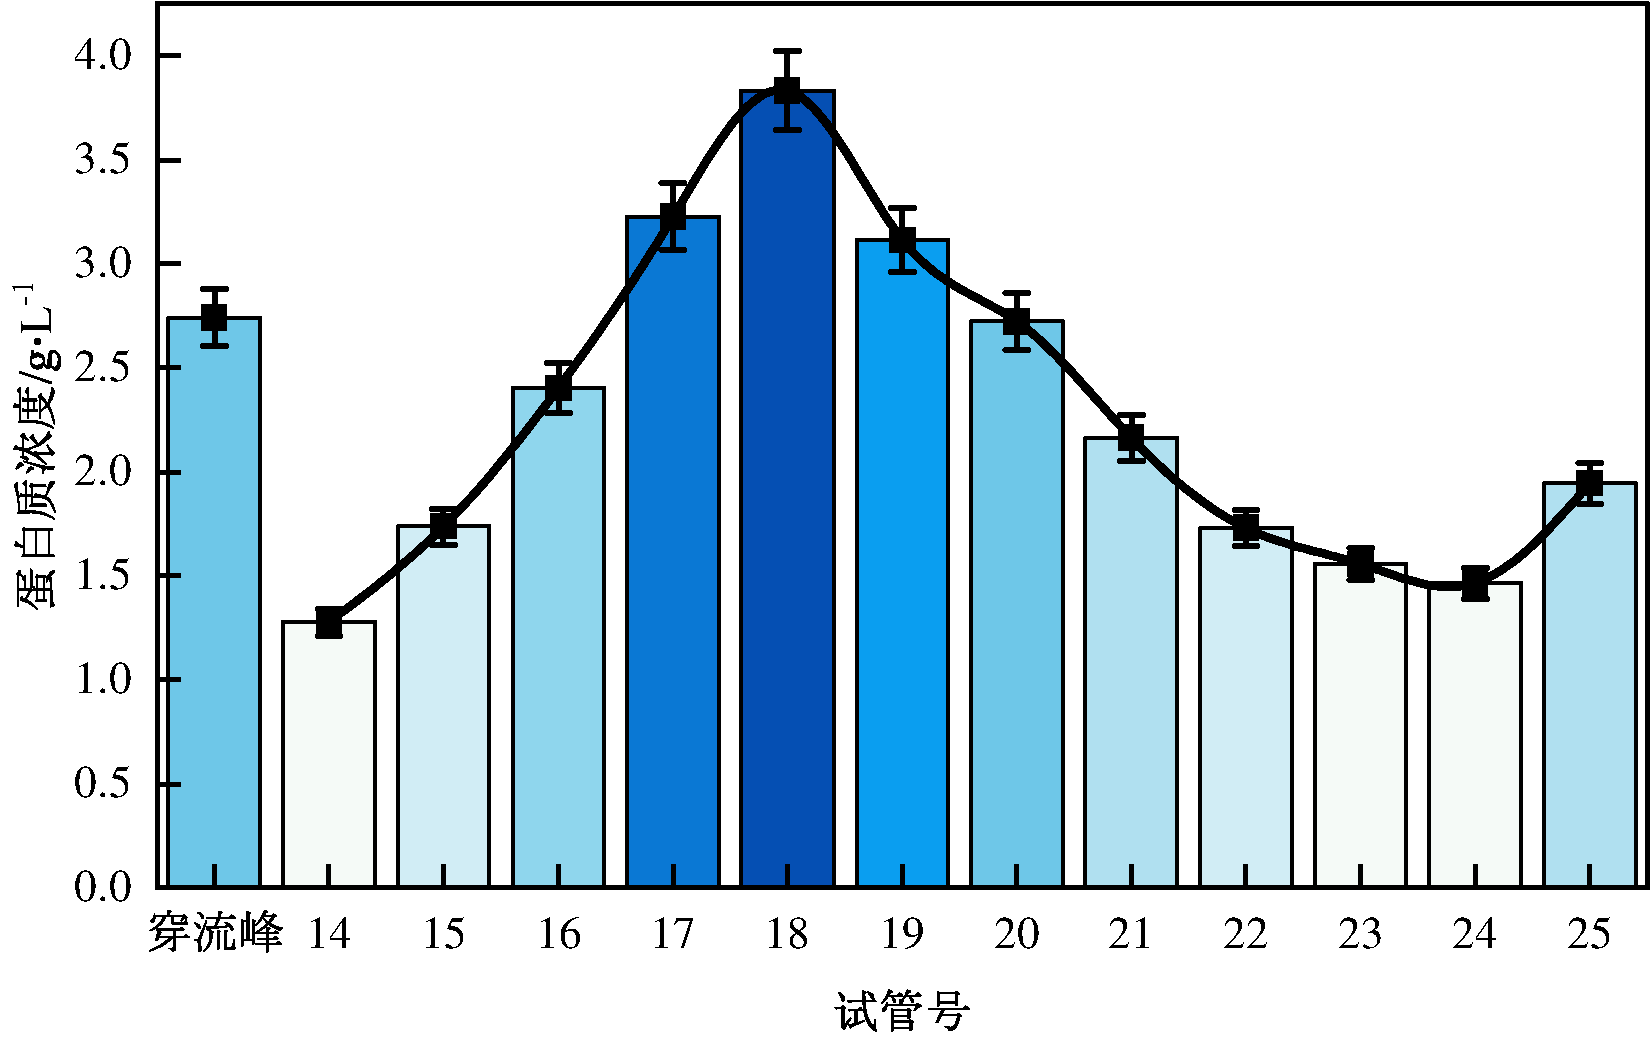
\includegraphics[width = \textwidth]{figure/1124/Pro_Curve.pdf}
        \caption{蛋白质洗脱曲线}
        \label{fig:Pro_Curve}
    \end{minipage}
\end{figure}

\subsection{酶活性的测定}

\begin{table}[H]
\centering
\caption{葡萄糖标准曲线绘制实验结果}
\label{tab:result_GLUCOSE_STD}
\begin{tabular}{@{}ccccccc@{}}
\toprule
试管号       & 1     & 2     & 3     & 4     & 5     & 6     \\ \midrule
葡萄糖浓度/$10^{-2}\mathrm{g \cdot L^{-1}}$    & 0.000 & 1.333 & 2.667 & 4.000 & 5.333 & 6.667 \\
520nm下吸光度 & 0.000 & 0.043 & 0.206 & 0.383 & 0.574 & 0.745 \\ \bottomrule
\end{tabular}
\end{table}

\begin{figure}[H]
    \centering
    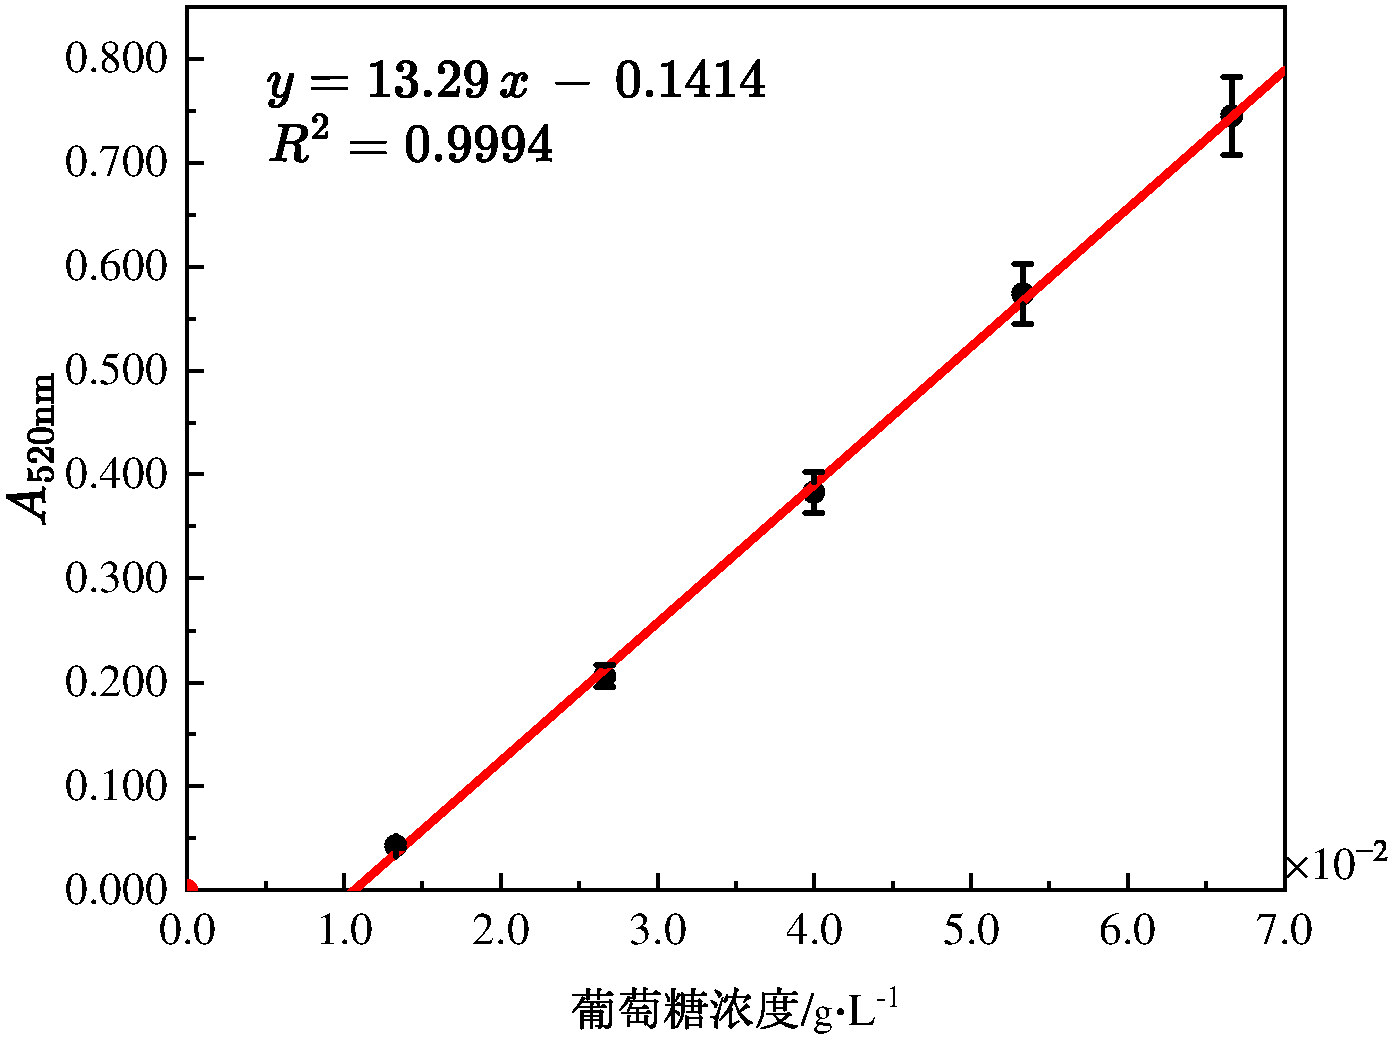
\includegraphics[width = 0.5\textwidth]{figure/1124/Glucose_STD.pdf}
    \caption{葡萄糖标准浓度曲线}
    \label{fig:STD_Glucose}
\end{figure}

\begin{figure}[H]
    \centering
    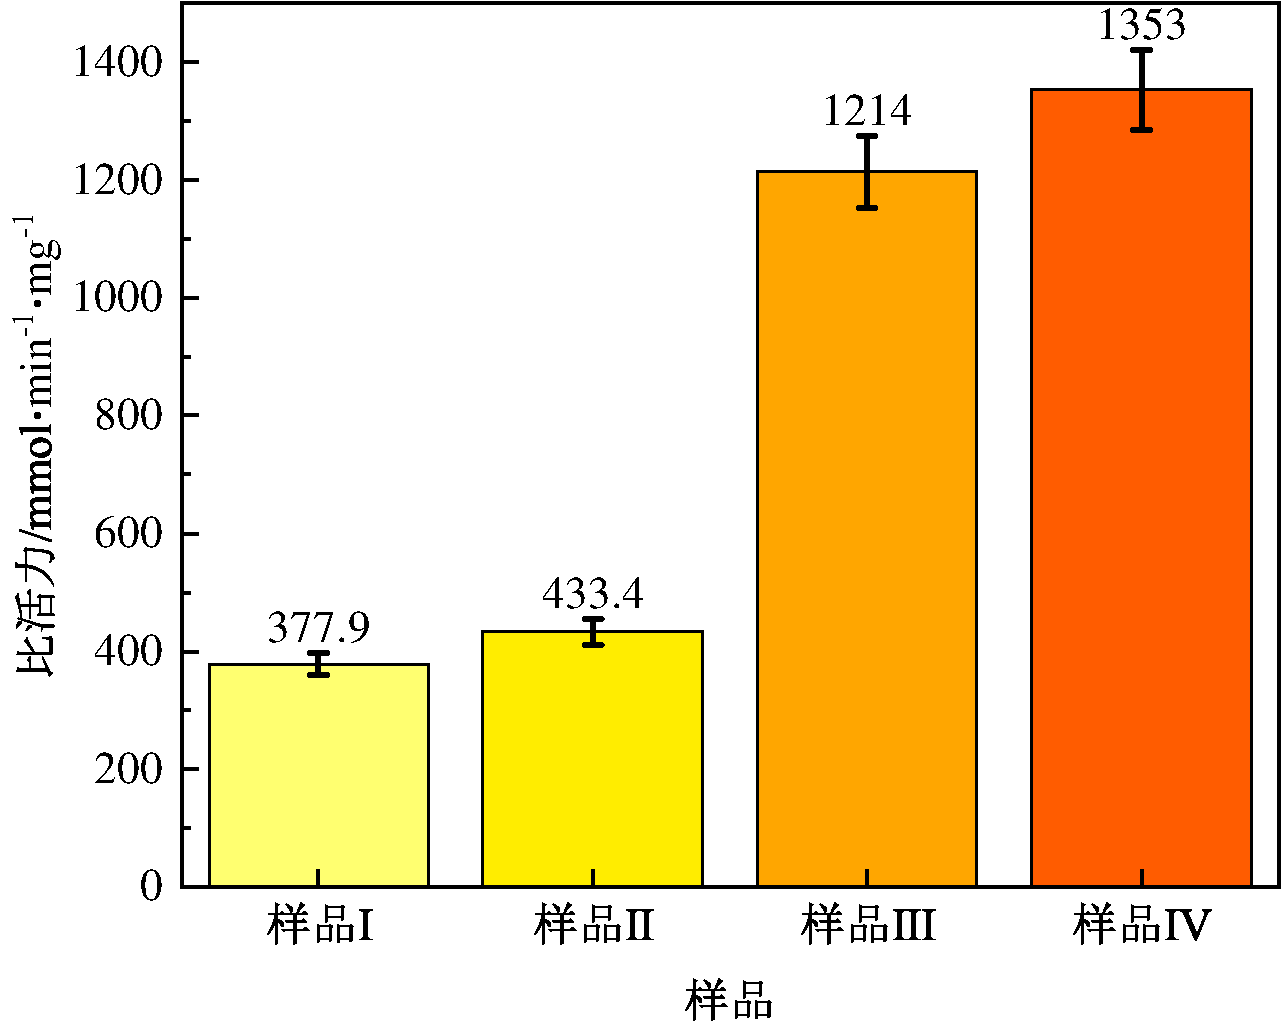
\includegraphics[width = 0.5\textwidth]{figure/1124/Activity_Sample.pdf}
    \caption{样本比活力}
    \label{fig:Activity_Sample}
\end{figure}

\begin{figure}[H]
    \centering
    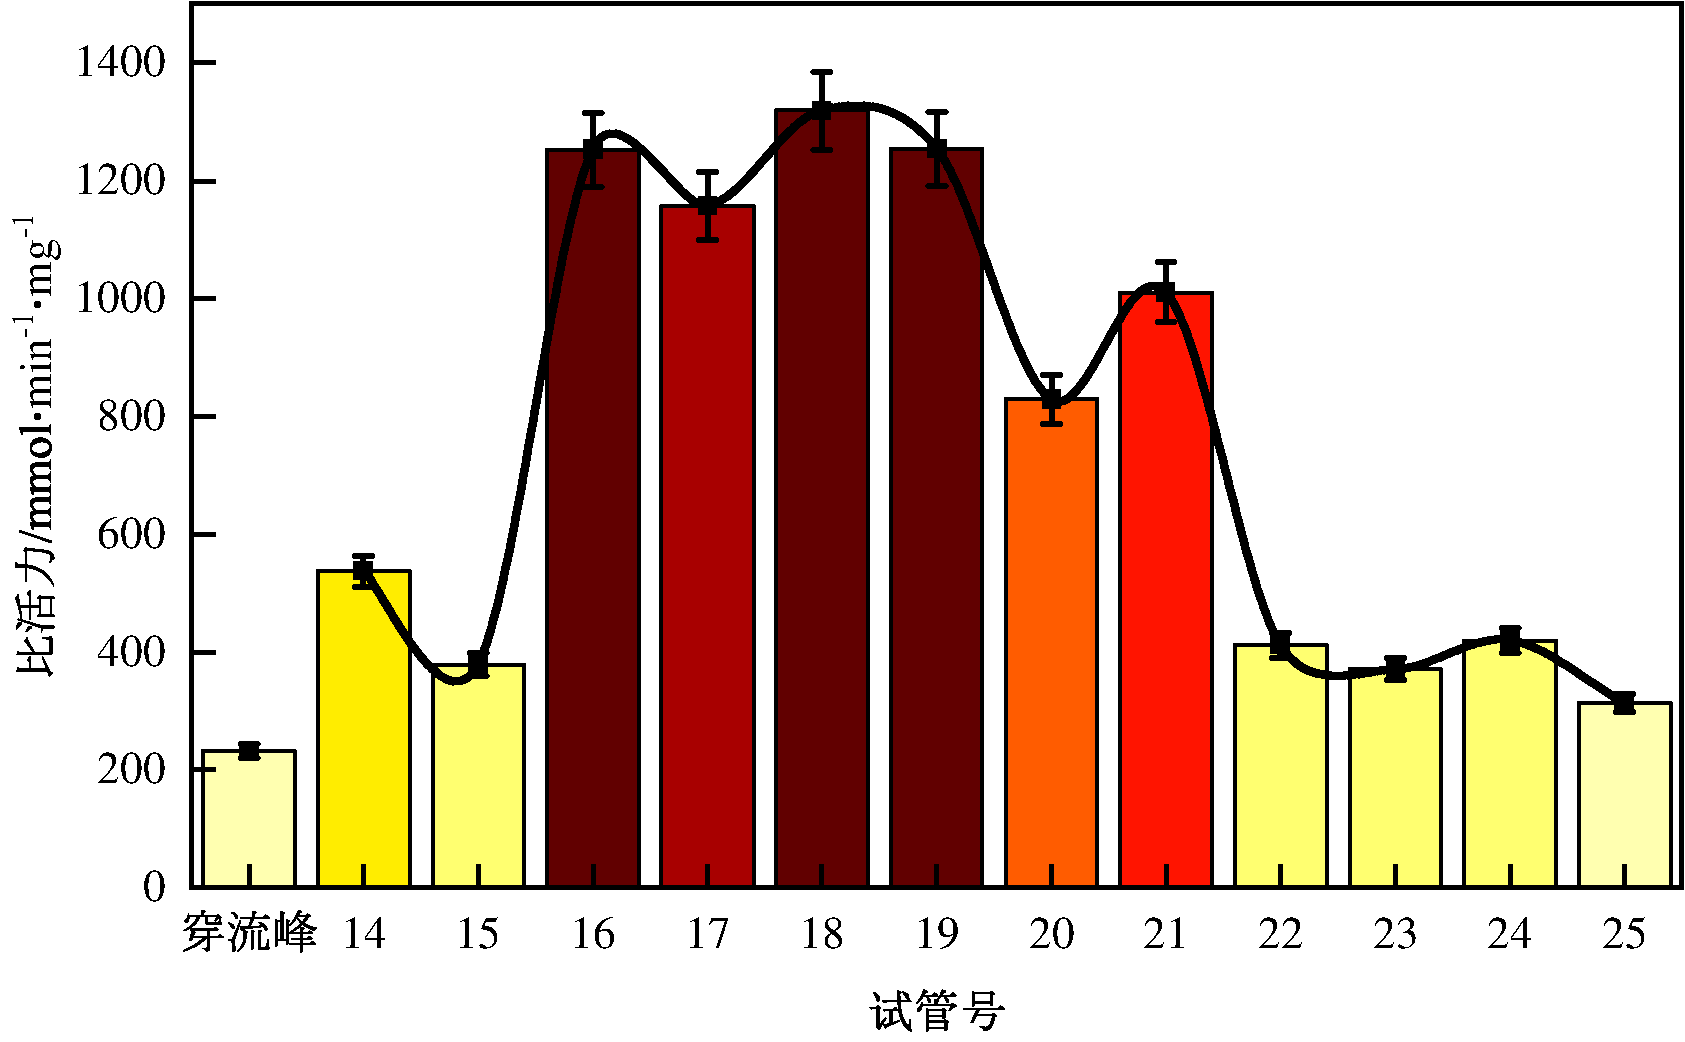
\includegraphics[width = 0.5\textwidth]{figure/1124/Activity_Curve.pdf}
    \caption{洗脱曲线比活力}
    \label{fig:Activity_Curve}
\end{figure}

\subsection{蔗糖酶酶切去糖基化}

\subsection{正交试验探究最佳反应条件}
本小组根据前期的相关实验数据和实验室提供的经验建议方案,确定了因素[E]、[S]的水平,结合实验室提供的T、pH的水平,三名组员根据自己选择的排列顺序确定了各自的表头,三组实验同时进行共同寻找优水平组合。

\begin{enumerate}
    \item 杨云翔的正交试验
    
\begin{table}[H]
\centering
\caption{杨云翔选择的正交试验表头}
\label{tab:my-table}
\begin{tabular}{|c|p{4em}<{\centering}|p{4em}<{\centering}|p{4em}<{\centering}|p{4em}<{\centering}|}
\hline \diagbox{水平}{因素}
 & \begin{tabular}[c]{@{}c@{}}{[}S{]}\\ /mL\end{tabular} & \begin{tabular}[c]{@{}c@{}}{[}E{]}\\ /mL\end{tabular} & \begin{tabular}[c]{@{}c@{}}温度\\ /\dc \end{tabular} & pH值 \\ \hline
水平I   & 0.5 & 0.037 & 50 & 4.6 \\ \hline
水平II  & 0.2 & 0.024 & 37 & 3.6 \\ \hline
水平III & 1.0 & 0.050 & 65 & 5.4 \\ \hline
\end{tabular}
\end{table}

\setlength{\parindent}{2em}根据其设计的表头,填入到$L^{9}(3^{4})$正交表中,得到各组的实验条件。按照预先设定开展实验后,在$\lambda=520\mathrm{nm}$下测定其吸光度。

\begin{table}[H]
\centering
\caption{杨云翔的各组实验条件及吸光度测定结果}
\label{tab:my-table}
\resizebox{\textwidth}{!}{
\begin{tabular}{l|c|cccccccccc|}
\cline{2-12}
 &
   &
  \multicolumn{1}{c|}{\textbf{2}} &
  \multicolumn{1}{c|}{\textbf{4}} &
  \multicolumn{1}{c|}{\textbf{9}} &
  \multicolumn{1}{c|}{\textbf{1}} &
  \multicolumn{1}{c|}{\textbf{6}} &
  \multicolumn{1}{c|}{\textbf{8}} &
  \multicolumn{1}{c|}{\textbf{3}} &
  \multicolumn{1}{c|}{\textbf{5}} &
  \multicolumn{1}{c|}{\textbf{7}} &
  \textbf{参比} \\ \cline{2-12} 
 &
  \textbf{\begin{tabular}[c]{@{}c@{}}5\%蔗糖溶液{[}S{]}\\ /mL\end{tabular}} &
  \multicolumn{1}{c|}{0.5} &
  \multicolumn{1}{c|}{0.2} &
  \multicolumn{1}{c|}{1} &
  \multicolumn{1}{c|}{0.5} &
  \multicolumn{1}{c|}{0.2} &
  \multicolumn{1}{c|}{1} &
  \multicolumn{1}{c|}{0.5} &
  \multicolumn{1}{c|}{0.2} &
  \multicolumn{1}{c|}{1} &
  0.5 \\ \cline{2-12} 
 &
  \textbf{{[}不同pH{]}} &
  \multicolumn{1}{c|}{pH5.4} &
  \multicolumn{1}{c|}{pH3.6} &
  \multicolumn{1}{c|}{pH4.6} &
  \multicolumn{1}{c|}{pH4.6} &
  \multicolumn{1}{c|}{pH5.4} &
  \multicolumn{1}{c|}{pH3.6} &
  \multicolumn{1}{c|}{pH3.6} &
  \multicolumn{1}{c|}{pH4.6} &
  \multicolumn{1}{c|}{pH5.4} &
  pH4.6 \\ \cline{2-12} 
 &
  \textbf{\begin{tabular}[c]{@{}c@{}}0.1mol/L 缓冲溶液\\ /mL\end{tabular}} &
  \multicolumn{1}{c|}{0.5} &
  \multicolumn{1}{c|}{0.5} &
  \multicolumn{1}{c|}{0.5} &
  \multicolumn{1}{c|}{0.5} &
  \multicolumn{1}{c|}{0.5} &
  \multicolumn{1}{c|}{0.5} &
  \multicolumn{1}{c|}{0.5} &
  \multicolumn{1}{c|}{0.5} &
  \multicolumn{1}{c|}{0.5} &
  0.5 \\ \cline{2-12} 
 &
  \textbf{\begin{tabular}[c]{@{}c@{}}去离子水\\ /mL\end{tabular}} &
  \multicolumn{1}{c|}{0.976} &
  \multicolumn{1}{c|}{1.263} &
  \multicolumn{1}{c|}{0.450} &
  \multicolumn{1}{c|}{0.963} &
  \multicolumn{1}{c|}{1.250} &
  \multicolumn{1}{c|}{0.476} &
  \multicolumn{1}{c|}{0.95} &
  \multicolumn{1}{c|}{1.276} &
  \multicolumn{1}{c|}{0.463} &
  1.000 \\ \cline{2-12} 
 &
  \textbf{\begin{tabular}[c]{@{}c@{}}样品IV蔗糖酶稀释液{[}E{]}\\ /mL\\ (需作相应预温)\end{tabular}} &
  \multicolumn{1}{c|}{0.024} &
  \multicolumn{1}{c|}{0.037} &
  \multicolumn{1}{c|}{0.050} &
  \multicolumn{1}{c|}{0.037} &
  \multicolumn{1}{c|}{0.050} &
  \multicolumn{1}{c|}{0.024} &
  \multicolumn{1}{c|}{0.050} &
  \multicolumn{1}{c|}{0.024} &
  \multicolumn{1}{c|}{0.037} &
  0.000 \\ \cline{2-12} 
 &
  \textbf{\begin{tabular}[c]{@{}c@{}}反应体系总体积\\ /mL\end{tabular}} &
  \multicolumn{1}{c|}{2} &
  \multicolumn{1}{c|}{2} &
  \multicolumn{1}{c|}{2} &
  \multicolumn{1}{c|}{2} &
  \multicolumn{1}{c|}{2} &
  \multicolumn{1}{c|}{2} &
  \multicolumn{1}{c|}{2} &
  \multicolumn{1}{c|}{2} &
  \multicolumn{1}{c|}{2} &
  2 \\ \cline{2-12} 
 &
  \textbf{【酶促反应】} &
  \multicolumn{3}{c|}{混匀,37\dc 保温10min} &
  \multicolumn{3}{c|}{混匀后,50\dc 保温10min} &
  \multicolumn{3}{c|}{混匀,65\dc 保温10min} &
   \\ \cline{2-12} 
 &
  \textbf{\begin{tabular}[c]{@{}c@{}}DNS试剂\\ /mL\end{tabular}} &
  \multicolumn{1}{c|}{0.5} &
  \multicolumn{1}{c|}{0.5} &
  \multicolumn{1}{c|}{0.5} &
  \multicolumn{1}{c|}{0.5} &
  \multicolumn{1}{c|}{0.5} &
  \multicolumn{1}{c|}{0.5} &
  \multicolumn{1}{c|}{0.5} &
  \multicolumn{1}{c|}{0.5} &
  \multicolumn{1}{c|}{0.5} &
  0.5 \\ \cline{2-12} 
 &
  \textbf{【显色】} &
  \multicolumn{10}{c|}{混匀,100\dc 水浴保温5min} \\ \cline{2-12} 
 &
  \textbf{\begin{tabular}[c]{@{}c@{}}去离子水\\ /mL\end{tabular}} &
  \multicolumn{1}{c|}{5} &
  \multicolumn{1}{c|}{5} &
  \multicolumn{1}{c|}{5} &
  \multicolumn{1}{c|}{5} &
  \multicolumn{1}{c|}{5} &
  \multicolumn{1}{c|}{5} &
  \multicolumn{1}{c|}{5} &
  \multicolumn{1}{c|}{5} &
  \multicolumn{1}{c|}{5} &
  5 \\ \cline{2-12} 
 &
   &
  \multicolumn{10}{c|}{在涡旋仪上充分混匀(戴上手套,防止溶液溅出)} \\ \cline{2-12} 
 &
  \textbf{\begin{tabular}[c]{@{}c@{}}分光光度计检测\\ $A_{520}$\end{tabular}} &
  \multicolumn{1}{c|}{0.32} &
  \multicolumn{1}{c|}{0.732} &
  \multicolumn{1}{c|}{1.285} &
  \multicolumn{1}{c|}{1.822} &
  \multicolumn{1}{c|}{1.61} &
  \multicolumn{1}{c|}{0.81} &
  \multicolumn{1}{c|}{0.124} &
  \multicolumn{1}{c|}{-0.005} &
  \multicolumn{1}{c|}{0.005} &
  \textbf{校零} \\ \cline{2-12} 
\end{tabular}
}
\end{table}

极差$R$表示某因素在其取值范围内对实验指标影响变化的幅度。对于同水平数的正交试验,因素显著性主次可按其极差$R$的大小来确定。$R$越大,表示该因素的水平值变化对指标的影响越大,这个因素就越重要,反之亦然。

% Please add the following required packages to your d\dc ument preamble:
% \usepackage{booktabs}
\begin{table}[H]
\centering
\caption{杨云翔的正交试验的极差分析}
\label{tab:my-table}
\begin{tabular}{@{}clclclclclclclclcl@{}}
\toprule
\multicolumn{2}{c}{\textbf{\begin{tabular}[c]{@{}c@{}}因素\end{tabular}}} &
\multicolumn{2}{c}{\textbf{\begin{tabular}[c]{@{}c@{}}水平$\mathrm{I}$\\ $\sum K_{i}$\end{tabular}}} &
  \multicolumn{2}{c}{\textbf{\begin{tabular}[c]{@{}c@{}}水平$\mathrm{II}$\\ $\sum K_{i}$\end{tabular}}} &
  \multicolumn{2}{c}{\textbf{\begin{tabular}[c]{@{}c@{}}水平$\mathrm{III}$\\ $\sum K_{i}$\end{tabular}}} &
  \multicolumn{2}{c}{\textit{\textbf{\begin{tabular}[c]{@{}c@{}}水平$\mathrm{I}$\\ $k_i=\frac{K_i}{3}$\end{tabular}}}} &
  \multicolumn{2}{c}{\textit{\textbf{\begin{tabular}[c]{@{}c@{}}水平$\mathrm{II}$\\  $k_i=\frac{K_i}{3}$\end{tabular}}}} &
  \multicolumn{2}{c}{\textit{\textbf{\begin{tabular}[c]{@{}c@{}}水平$\mathrm{III}$\\  $k_i=\frac{K_i}{3}$\end{tabular}}}} &
  \multicolumn{2}{c}{\textbf{\begin{tabular}[c]{@{}c@{}}极差\\ $R$值\end{tabular}}} &
  \multicolumn{2}{c}{\textbf{主次顺序}} \\ \midrule
\multicolumn{2}{c}{[S]} &
 \multicolumn{2}{c}{2.266} &
  \multicolumn{2}{c}{2.337} &
  \multicolumn{2}{c}{2.1} &
  \multicolumn{2}{c}{0.755} &
  \multicolumn{2}{c}{0.799} &
  \multicolumn{2}{c}{0.7} &
  \multicolumn{2}{c}{0.079} &
  \multicolumn{2}{c}{4} \\
\multicolumn{2}{c}{[E]} &
 \multicolumn{2}{c}{2.559} &
  \multicolumn{2}{c}{1.125} &
  \multicolumn{2}{c}{3.019} &
  \multicolumn{2}{c}{0.853} &
  \multicolumn{2}{c}{0.375} &
  \multicolumn{2}{c}{1.006} &
  \multicolumn{2}{c}{0.631} &
  \multicolumn{2}{c}{2} \\
\multicolumn{2}{c}{T} &
 \multicolumn{2}{c}{4.242} &
  \multicolumn{2}{c}{2.337} &
  \multicolumn{2}{c}{0.124} &
  \multicolumn{2}{c}{1.414} &
  \multicolumn{2}{c}{0.779} &
  \multicolumn{2}{c}{0.041} &
  \multicolumn{2}{c}{1.373} &
  \multicolumn{2}{c}{1} \\
\multicolumn{2}{c}{pH} &
 \multicolumn{2}{c}{3.102} &
  \multicolumn{2}{c}{1.935} &
  \multicolumn{2}{c}{1.666} &
  \multicolumn{2}{c}{1.034} &
  \multicolumn{2}{c}{0.645} &
  \multicolumn{2}{c}{0.555} &
  \multicolumn{2}{c}{0.479} &
  \multicolumn{2}{c}{3} \\ \bottomrule
\end{tabular}
\end{table}

对测得的数据进行极差$R$分析判断因素显著性主次关系,通过极差对比,对各因素的影响程度显著性进行排序为:温度>酶浓度>pH>底物浓度。

以指标均值$k_i$为纵坐标,因素水平数为横坐标作图,可看出该因素对指标的影响趋势,其最大均值对应的水平即为该因素的最佳水平。

\begin{figure}[H]
    \centering
    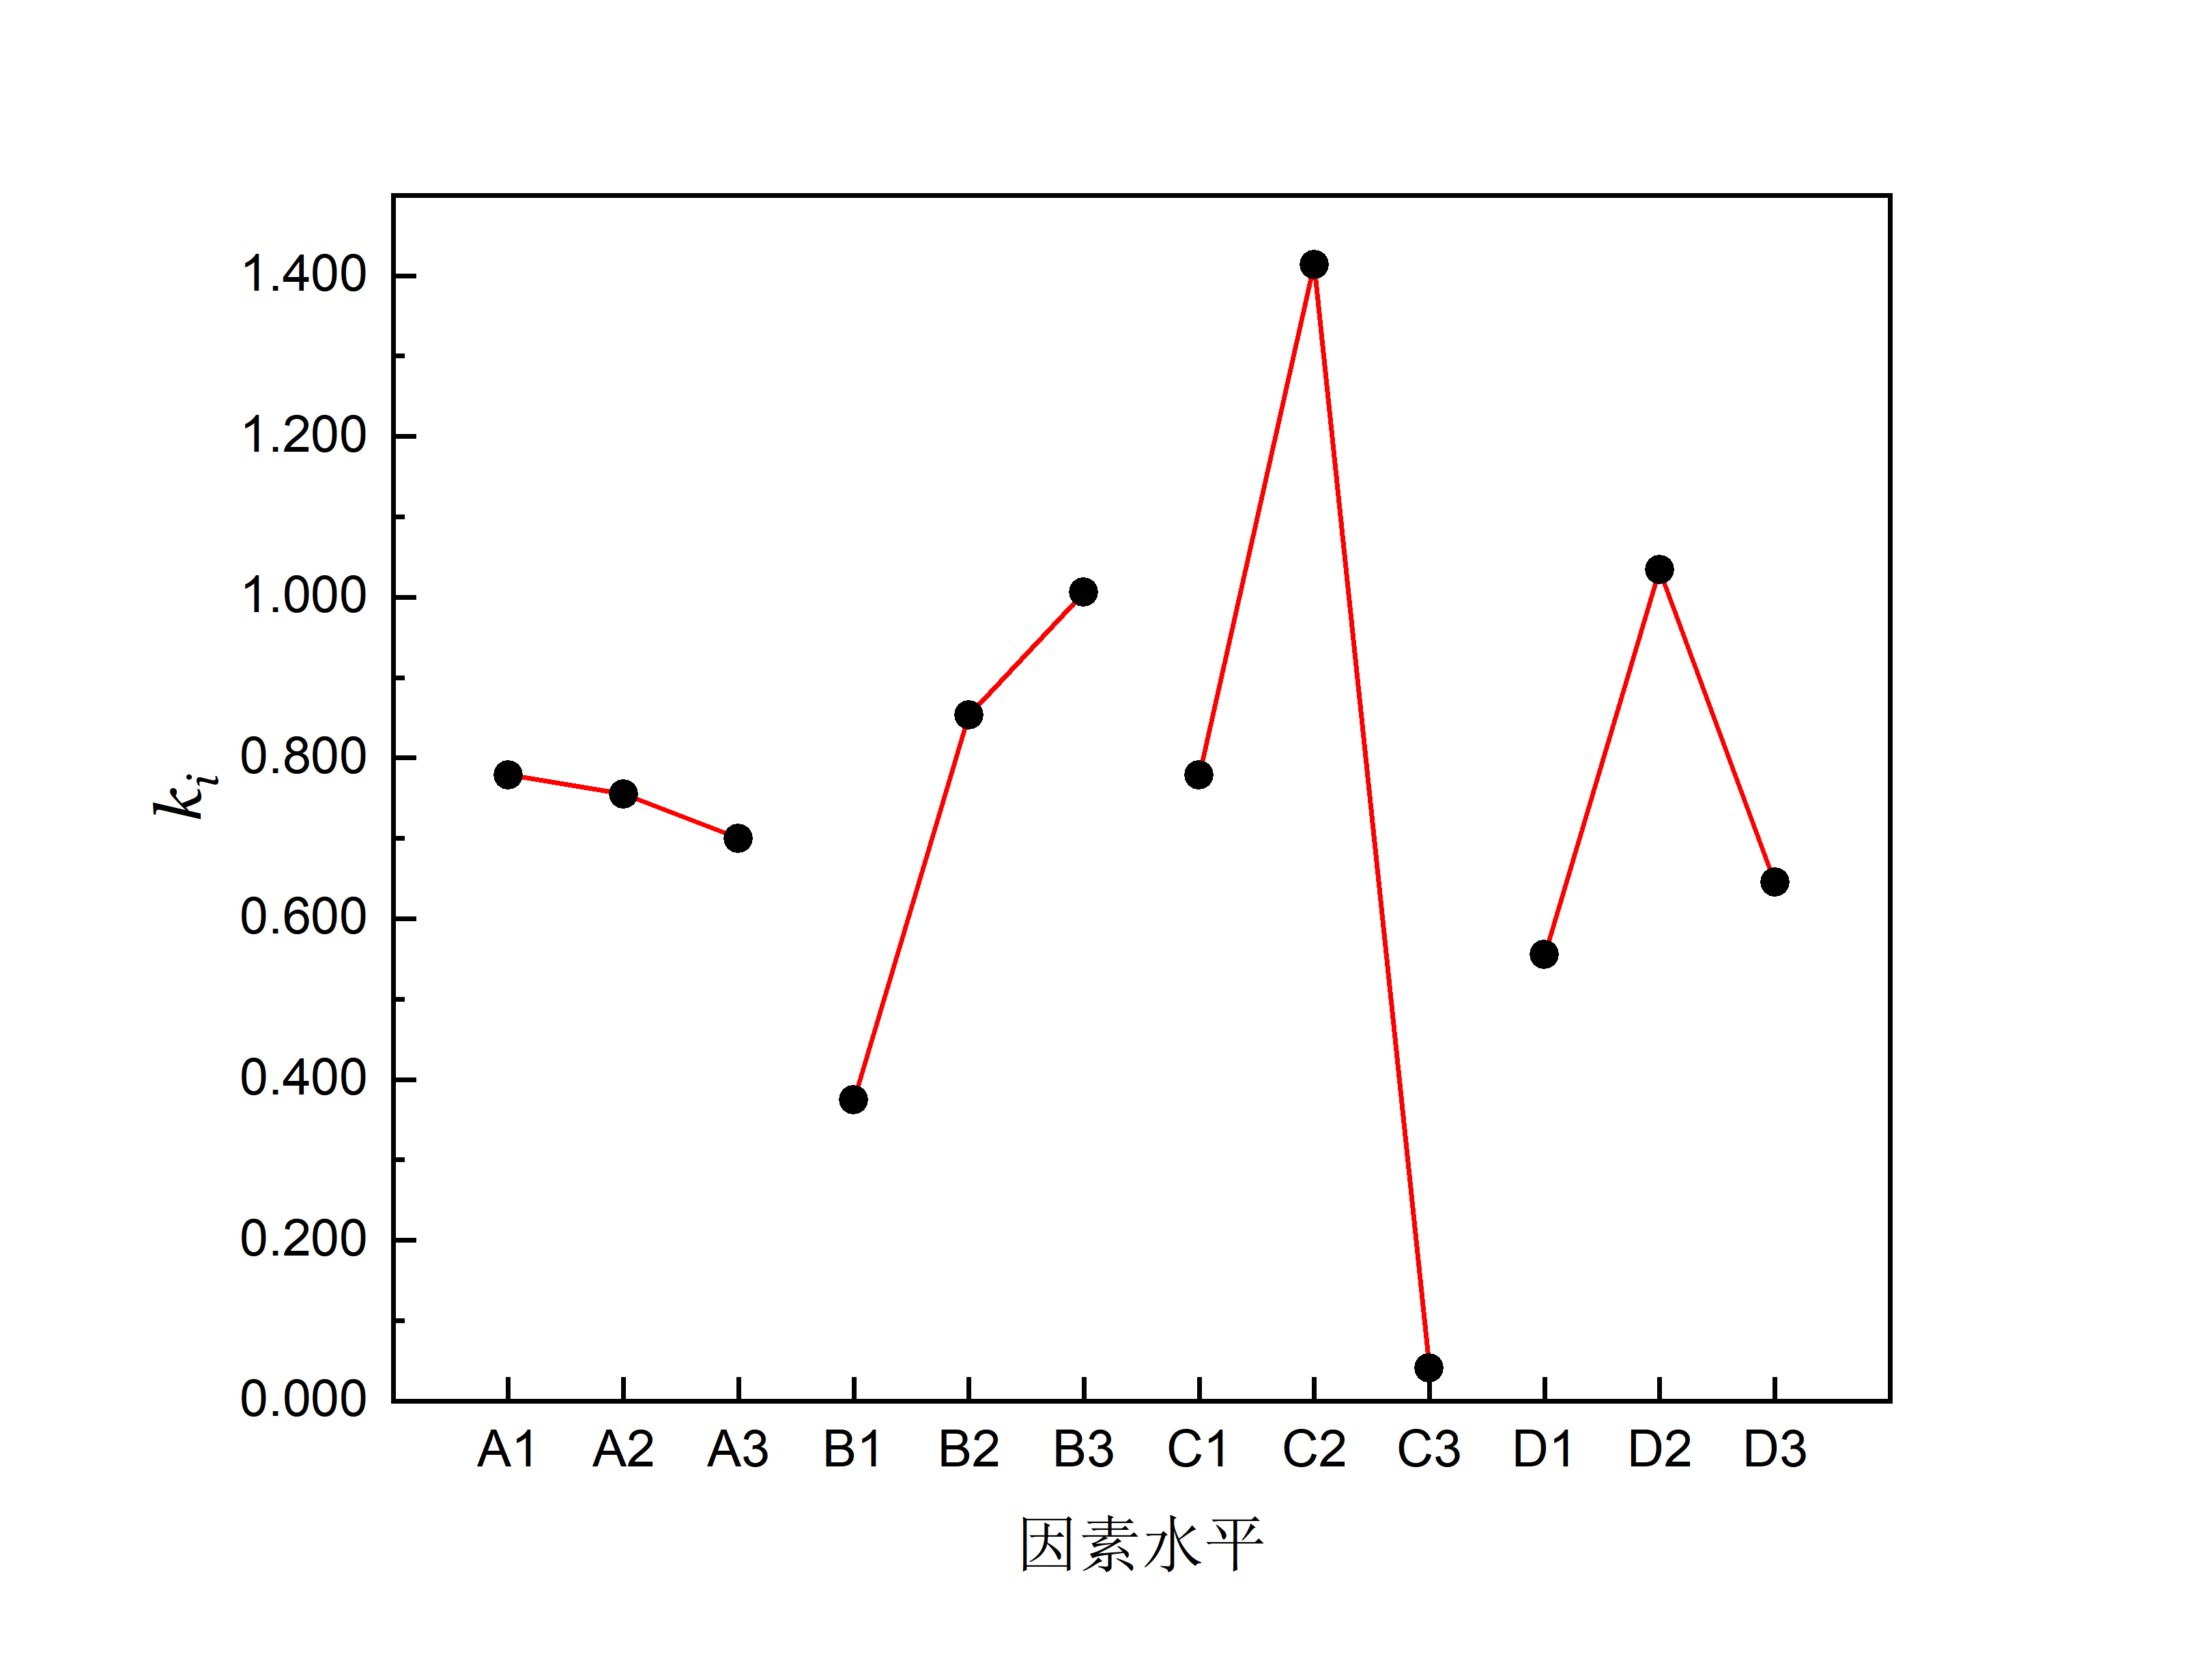
\includegraphics[width = 0.7\textwidth]{figure/Some Pictures/figure-1.png}
    \caption{杨云翔正交试验的指标-因素关系图}
    \label{fig:enter-label}
\end{figure}

根据绘制的图像可知,随着蔗糖的浓度增加,反而吸光度降低,可能在吸光度水平最高的地方取得蔗糖浓度的最优条件,但仍然需要进一步实验或分析确定;随着蔗糖酶浓度的增加,吸光度升高,可能在吸光度水平最高的地方取得蔗糖酶浓度的最优条件,但仍然需要进一步实验或分析确定;而在温度、pH值两个因素中,出现了最优条件的峰值,最优pH为4.6,最优温度为50$\dc$。同时,结合酶与底物作用的相关原理,蔗糖浓度一组的实验结果与理论分析存在一定偏差。因此,略去蔗糖浓度的因素,本正交试验确定的最优组合为[E]=0.050mL,T=50$\dc$,pH=4.6。

    \item 杨景媛的正交试验

\begin{table}[H]
\centering
\caption{杨景媛选择的正交试验表头}
\label{tab:my-table}
\begin{tabular}{|c|p{4em}<{\centering}|p{4em}<{\centering}|p{4em}<{\centering}|p{4em}<{\centering}|}
\hline \diagbox{水平}{因素}
 & \begin{tabular}[c]{@{}c@{}}{[}E{]}\\ /mL\end{tabular} & \begin{tabular}[c]{@{}c@{}}{[}S{]}\\ /mL\end{tabular} & \begin{tabular}[c]{@{}c@{}}温度\\ /\dc \end{tabular} & pH值 \\ \hline
水平I   & 0.024 & 1.0 & 50 & 5.4 \\ \hline
水平II  & 0.050 & 0.2 & 37 & 3.6 \\ \hline
水平III & 0.037 & 0.5 & 65 & 4.6 \\ \hline
\end{tabular}
\end{table}

根据确定下来的表头,填入到$L^{9}(3^{4})$正交表中,得到各组的实验条件。按照预先设定开展实验后,在$\lambda=520\mathrm{nm}$下测定其吸光度。

\begin{table}[H]
\centering
\caption{杨景媛的正交试验的各组试验条件与极差R值分析}
\label{tab:my-table}
\begin{tabular}{|c|c|c|c|c|c|}
\hline
\textbf{实验号}                  & \textbf{\begin{tabular}[c]{@{}c@{}}{[}S{]}\\ /mL\end{tabular}} & \textbf{\begin{tabular}[c]{@{}c@{}}{[}E{]}\\ /mL\end{tabular}} & \textbf{\begin{tabular}[c]{@{}c@{}}T\\ /\textbackslash{}dc\end{tabular}} & \textbf{pH值} & \textbf{试验结果} \\ \hline
1                             & 1.0                                                            & 0.024                                                          & 50                                                                       & 5.4          & 1.389         \\ \hline
2                             & 0.2                                                            & 0.024                                                          & 37                                                                       & 3.6          & 0.179         \\ \hline
3                             & 0.5                                                            & 0.024                                                          & 65                                                                       & 4.6          & 0.006         \\ \hline
4                             & 1.0                                                            & 0.050                                                          & 37                                                                       & 4.6          & 1.737         \\ \hline
5                             & 0.2                                                            & 0.050                                                          & 65                                                                       & 5.4          & -0.002        \\ \hline
6                             & 0.5                                                            & 0.050                                                          & 50                                                                       & 3.6          & 1.699         \\ \hline
7                             & 1.0                                                            & 0.037                                                          & 65                                                                       & 3.6          & 0.158         \\ \hline
8                             & 0.2                                                            & 0.037                                                          & 50                                                                       & 4.6          & 0.649         \\ \hline
9                             & 0.5                                                            & 0.037                                                          & 37                                                                       & 5.4          & 0.814         \\ \hline
\textbf{\begin{tabular}[c]{@{}c@{}}水平$\mathrm{I}$\\ $\sum K_{i}$\end{tabular}}              & 3.284                                                          & 1.574                                                          & 3.737                                                                    & 2.201        & \textbf{}     \\ \hline
\textbf{\begin{tabular}[c]{@{}c@{}}水平$\mathrm{II}$\\ $\sum K_{i}$\end{tabular}}              & 0.826                                                          & 3.434                                                          & 2.730                                                                    & 2.036        & \textbf{}     \\ \hline
\textbf{\begin{tabular}[c]{@{}c@{}}水平$\mathrm{III}$\\ $\sum K_{i}$\end{tabular}}              & 2.519                                                          & 1.621                                                          & 0.162                                                                    & 2.392        & \textbf{}     \\ \hline
\textit{\textbf{\begin{tabular}[c]{@{}c@{}}水平$\mathrm{I}$\\ $k_i=\frac{K_i}{3}$\end{tabular}}} & 1.095                                                          & 0.525                                                          & 1.246                                                                    & 0.734        & \textbf{}     \\ \hline
\textit{\textbf{\begin{tabular}[c]{@{}c@{}}水平$\mathrm{II}$\\ $k_i=\frac{K_i}{3}$\end{tabular}}} & 0.275                                                          & 1.145                                                          & 0.910                                                                    & 0.679        & \textbf{}     \\ \hline
\textit{\textbf{\begin{tabular}[c]{@{}c@{}}水平$\mathrm{III}$\\ $k_i=\frac{K_i}{3}$\end{tabular}}} & 0.840                                                          & 0.540                                                          & 0.054                                                                    & 0.797        & \textbf{}     \\ \hline
\textbf{极差R值}                 & 0.819                                                          & 0.620                                                          & 1.192                                                                    & 0.119        & \textbf{}     \\ \hline
\textbf{主次顺序}                 & 2                                                              & 3                                                              & 1                                                                        & 4            & \textbf{}     \\ \hline
\end{tabular}
\end{table}

根据极差$R$值分析结果显示,四个因素的显著性主次顺序为:温度>底物浓度>酶浓度>pH。再绘制指标-因素关系图进一步寻找最优组合。

\begin{figure}[H]
    \centering
    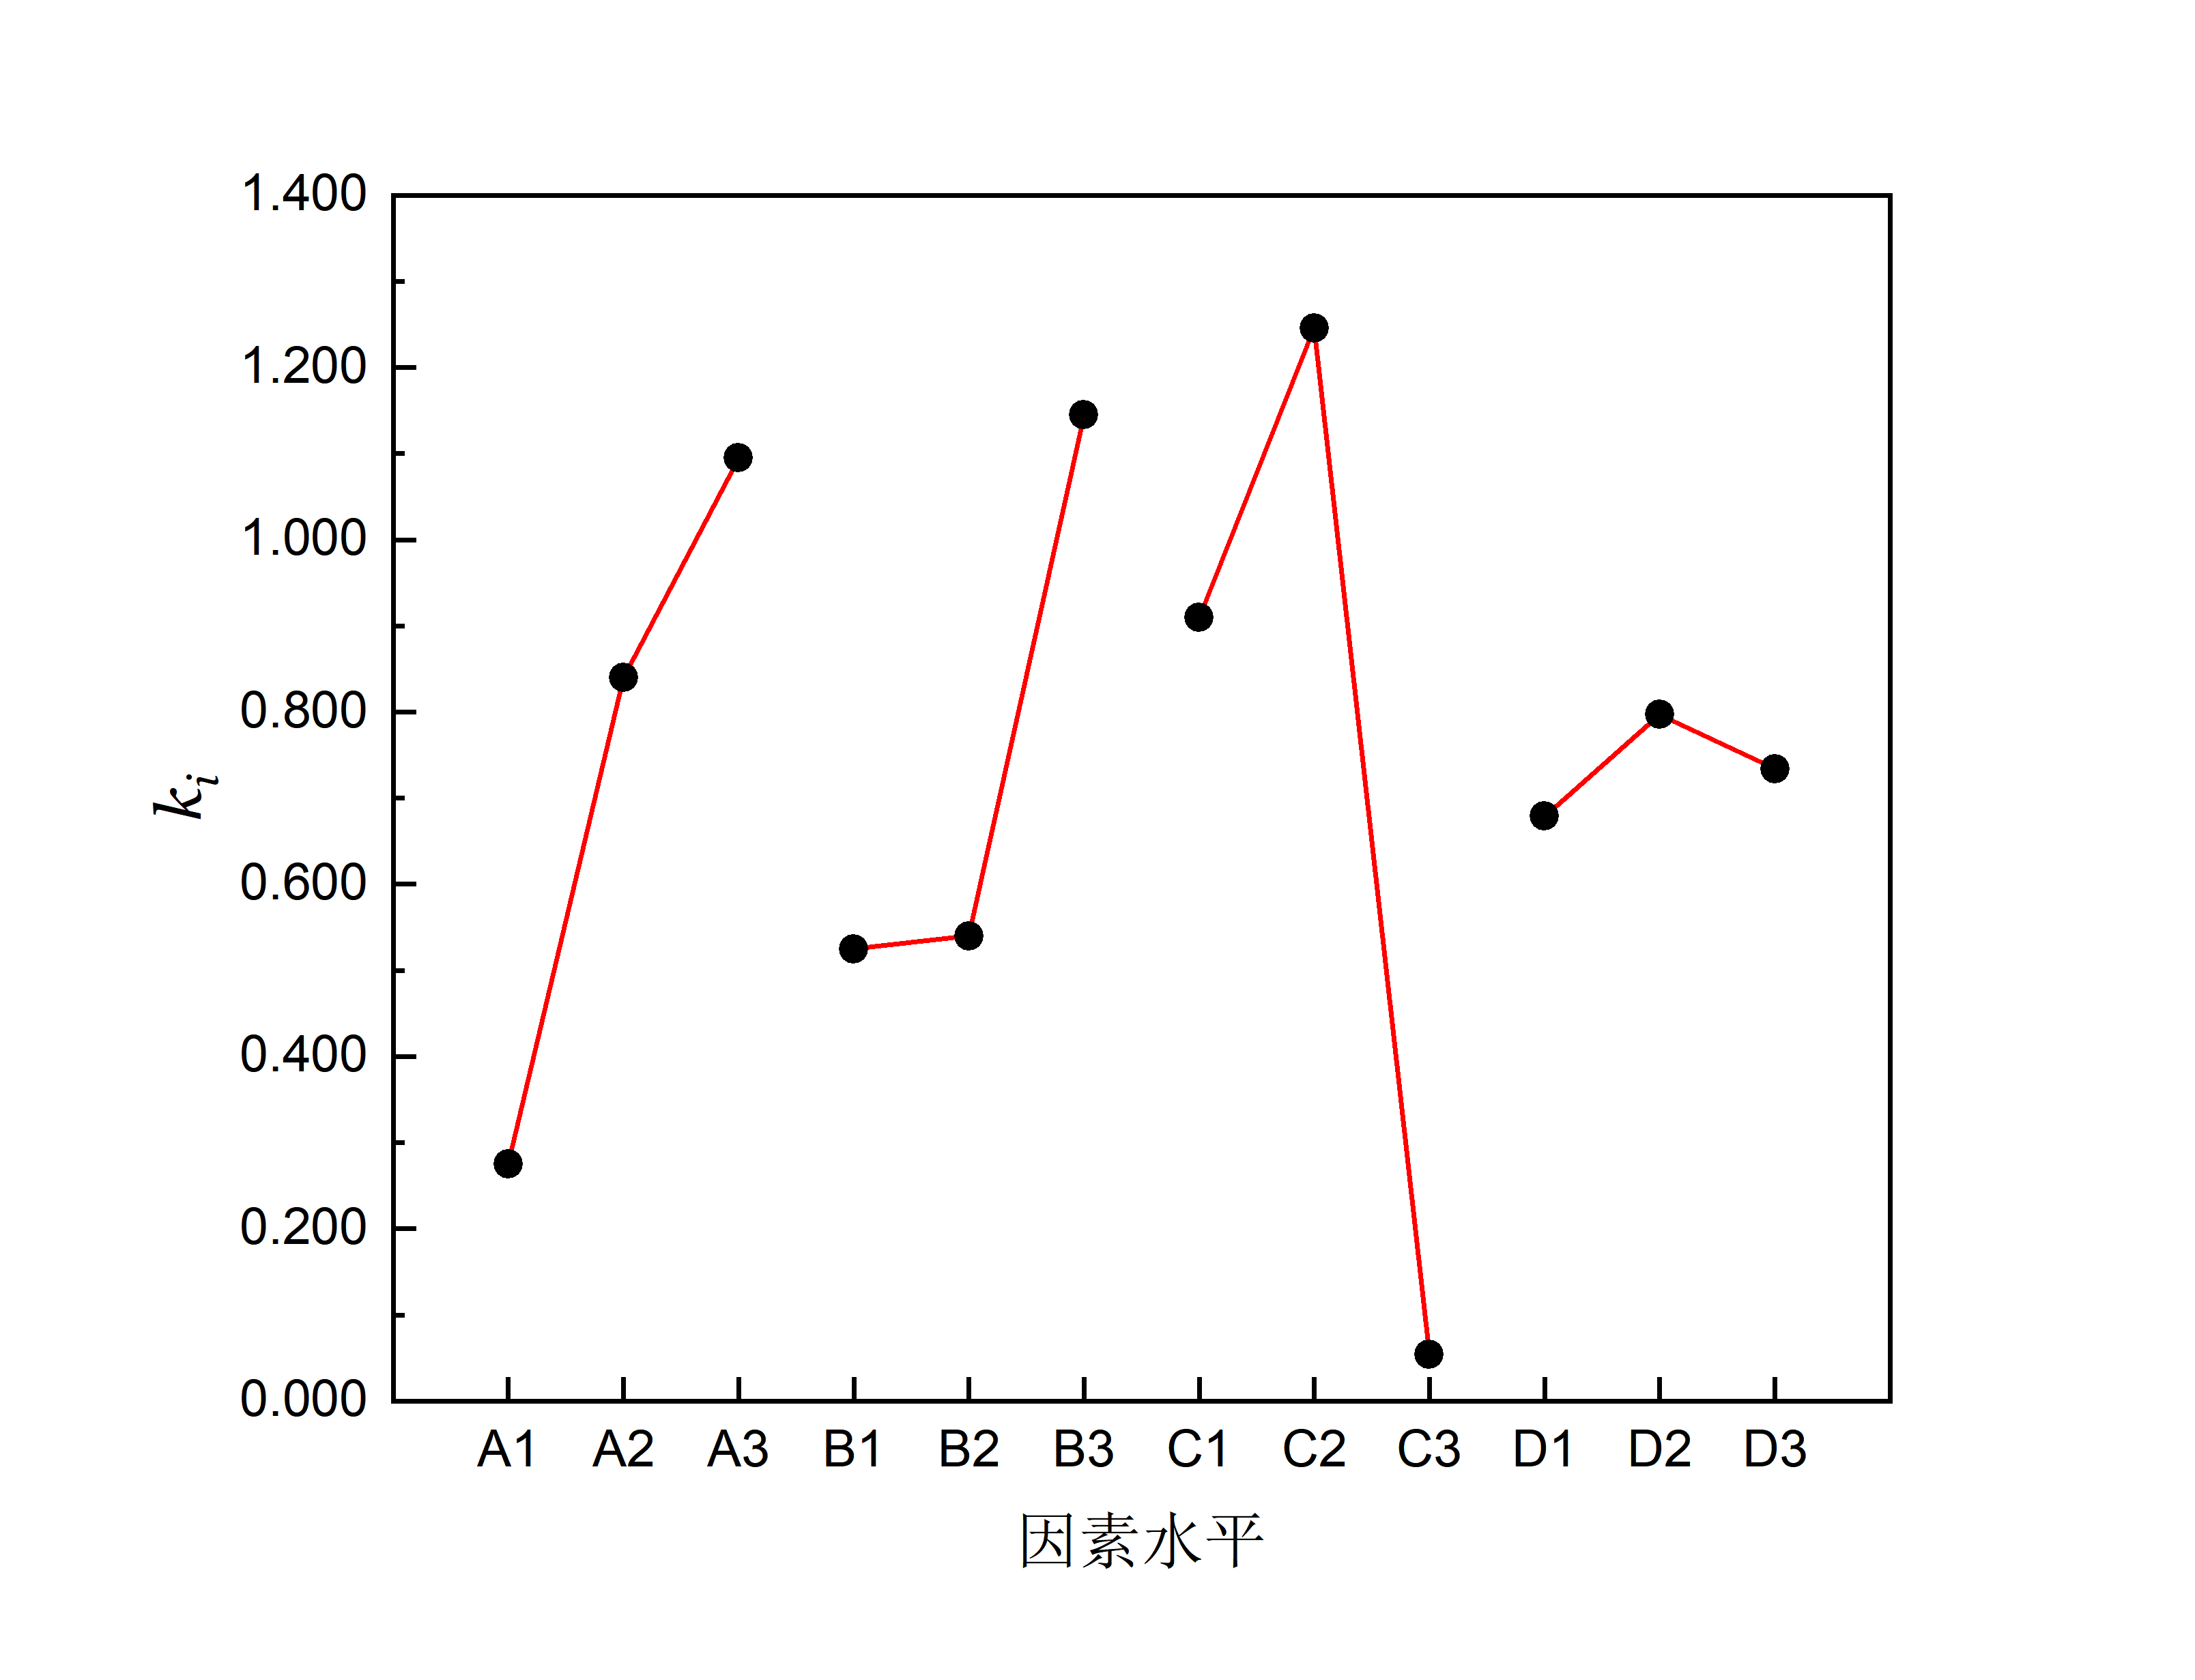
\includegraphics[width = 0.7\textwidth]{figure/Some Pictures/figure-2.png}
    \caption{杨景媛的正交试验的指标-因素关系图}
    \label{fig:enter-label}
\end{figure}

根据绘制的图像可知,随着蔗糖、蔗糖酶的浓度增加,反而吸光度降低,可能在吸光度水平最高的地方取得蔗糖浓度的最优条件,但仍然需要进一步实验或分析确定,而在温度、pH值两个因素中,出现了最优条件的峰值,最优pH为4.6,最优温度为50$\dc$。本正交试验确定的最优组合为[E]=0.050mL,[S]=0.050mL,T=50$\dc$,pH=4.6。

    \item 林雨泽的正交试验

\begin{table}[H]
\centering
\caption{林雨泽选择的正交试验表头}
\label{tab:my-table}
\begin{tabular}{|c|c|c|c|c|}
    \hline \diagbox{水平}{因素}
 & \begin{tabular}[c]{@{}c@{}}{[}S{]}\\ /mL\end{tabular} & \begin{tabular}[c]{@{}c@{}}{[}E{]}\\ /mL\end{tabular} & pH值 & \begin{tabular}[c]{@{}c@{}}温度\\ /\dc\end{tabular} \\ \hline
水平I & 0.5 & 0.037 & 4.6 & 50 \\ \hline
水平II & 0.2 & 0.024 & 5.4 & 37 \\ \hline
水平III & 1.0 & 0.050 & 3.6 & 65 \\ \hline
\end{tabular}
\end{table}

根据确定下来的表头,填入到$L^{9}(3^{4})$正交表中,得到各组的实验条件。按照预先设定开展实验后,在$\lambda=520\mathrm{nm}$下测定其吸光度。

\begin{table}[H]
\centering
\caption{林雨泽的正交试验的各组试验条件与极差R值分析}
\label{tab:my-table}
\begin{tabular}{|c|c|c|c|c|c|}
\hline
\textbf{实验号}                      & \textbf{{[}S{]}} & \textbf{{[}E{]}} & \textbf{pH值} & \textbf{温度} & \textbf{测量值} \\ \hline
1                                 & 0.5              & 0.037            & 4.6          & 50          & 1.702        \\ \hline
2                                 & 0.5              & 0.024            & 5.4          & 37          & 0.729        \\ \hline
3                                 & 0.5              & 0.050            & 3.6          & 65          & 0.089        \\ \hline
4                                 & 0.2              & 0.037            & 5.4          & 65          & -0.01        \\ \hline
5                                 & 0.2              & 0.024            & 3.6          & 50          & 0.345        \\ \hline
6                                 & 0.2              & 0.050            & 4.6          & 37          & 0.705        \\ \hline
7                                 & 1.0              & 0.037            & 3.6          & 37          & 1.423        \\ \hline
8                                 & 1.0              & 0.024            & 4.6          & 65          & 0.017        \\ \hline
9                                 & 1.0              & 0.050            & 5.4          & 50          & 2.976        \\ \hline
\textbf{\begin{tabular}[c]{@{}c@{}}水平$\mathrm{I}$\\ $\sum K_{i}$\end{tabular}}                    & 2.520            & 3.115            & 2.424        & 5.023       &              \\ \hline
\textbf{\begin{tabular}[c]{@{}c@{}}水平$\mathrm{II}$\\ $\sum K_{i}$\end{tabular}}                    & 1.040            & 1.091            & 3.695        & 2.857       &              \\ \hline
\textbf{\begin{tabular}[c]{@{}c@{}}水平$\mathrm{III}$\\ $\sum K_{i}$\end{tabular}}                    & 4.416            & 3.770            & 1.857        & 0.096       &              \\ \hline
\textbf{\begin{tabular}[c]{@{}c@{}}水平$\mathrm{I}$\\ $k_i=\frac{K_i}{3}$\end{tabular}}                     & 0.840            & 1.038            & 0.808        & 1.674       &              \\ \hline
\textbf{\begin{tabular}[c]{@{}c@{}}水平$\mathrm{II}$\\ $k_i=\frac{K_i}{3}$\end{tabular}}                     & 0.347            & 0.364            & 1.232        & 0.952       &              \\ \hline
\textbf{\begin{tabular}[c]{@{}c@{}}水平$\mathrm{III}$\\ $k_i=\frac{K_i}{3}$\end{tabular}}                     & 1.472            & 1.257            & 0.619        & 0.032       &              \\ \hline
\textbf{$R$}                        & 1.125            & 0.893            & 0.449        & 1.642       &              \\ \hline
\multicolumn{1}{|l|}{\textbf{主次顺序}} & 2                & 3                & 4            & 1           &              \\ \hline
\end{tabular}
\end{table}

根据极差$R$值分析结果显示,四个因素的显著性主次顺序为:温度>底物浓度>酶浓度>pH。再绘制指标-因素关系图进一步寻找最优组合。

\begin{figure}[H]
    \centering
    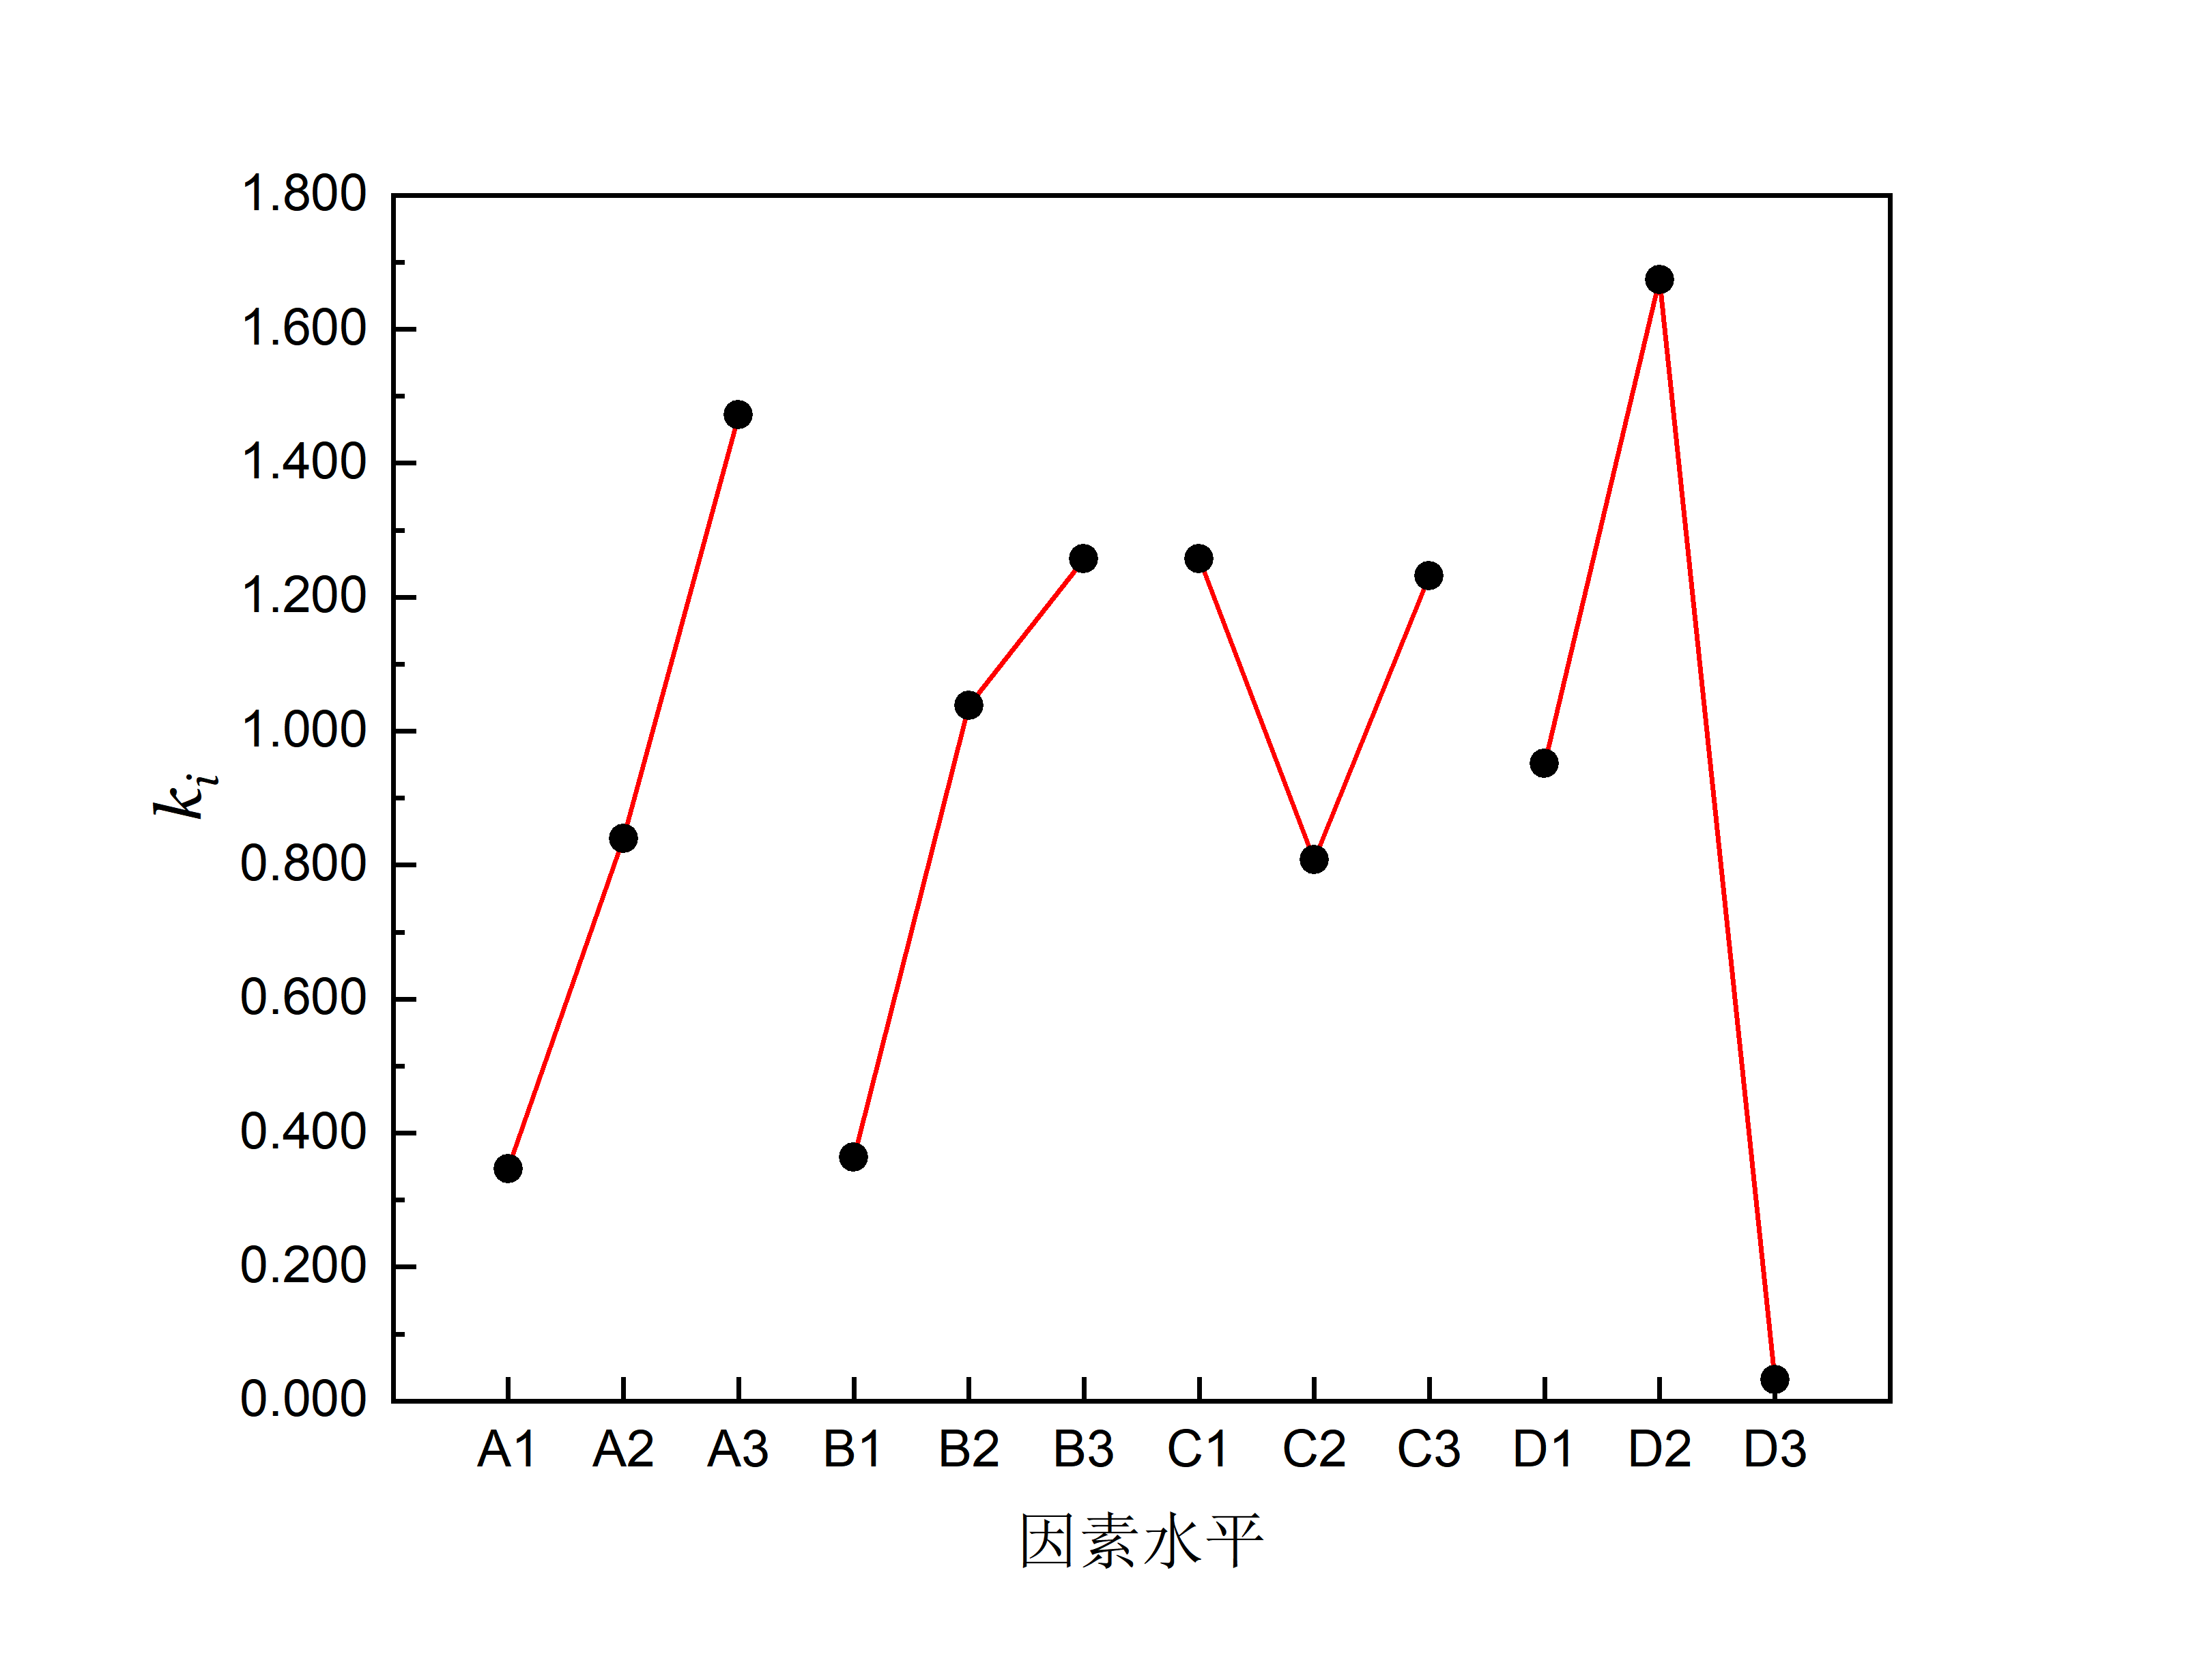
\includegraphics[width = 0.7\textwidth]{figure/Some Pictures/figure-3.png}
    \caption{林雨泽的正交试验的指标-因素关系图}
    \label{fig:enter-label}
\end{figure}

根据绘制的图像可知,随着蔗糖、蔗糖酶的浓度增加,反而吸光度降低,可能在吸光度水平最高的地方取得蔗糖浓度的最优条件,但仍然需要进一步实验或分析确定,温度出现了最优条件的峰值,最优温度为50$\dc$;而pH的因素-$k_i$曲线呈现下凹的趋势,无法得出最优条件。因此,除去因素pH,本正交试验确定的最优组合为[E]=0.050mL,[S]=0.050mL,T=50$\dc$。

\end{enumerate}

根据三个正交试验的R值分析结果,结合理论分析,得出蔗糖浓度、蔗糖酶浓度、温度、pH对酶促反应影响的显著性主次关系为:温度>底物(蔗糖)浓度>酶(蔗糖酶)浓度>pH。将三组正交试验的数据联合作指标-因素图如下。

\begin{figure}[H]
    \centering
    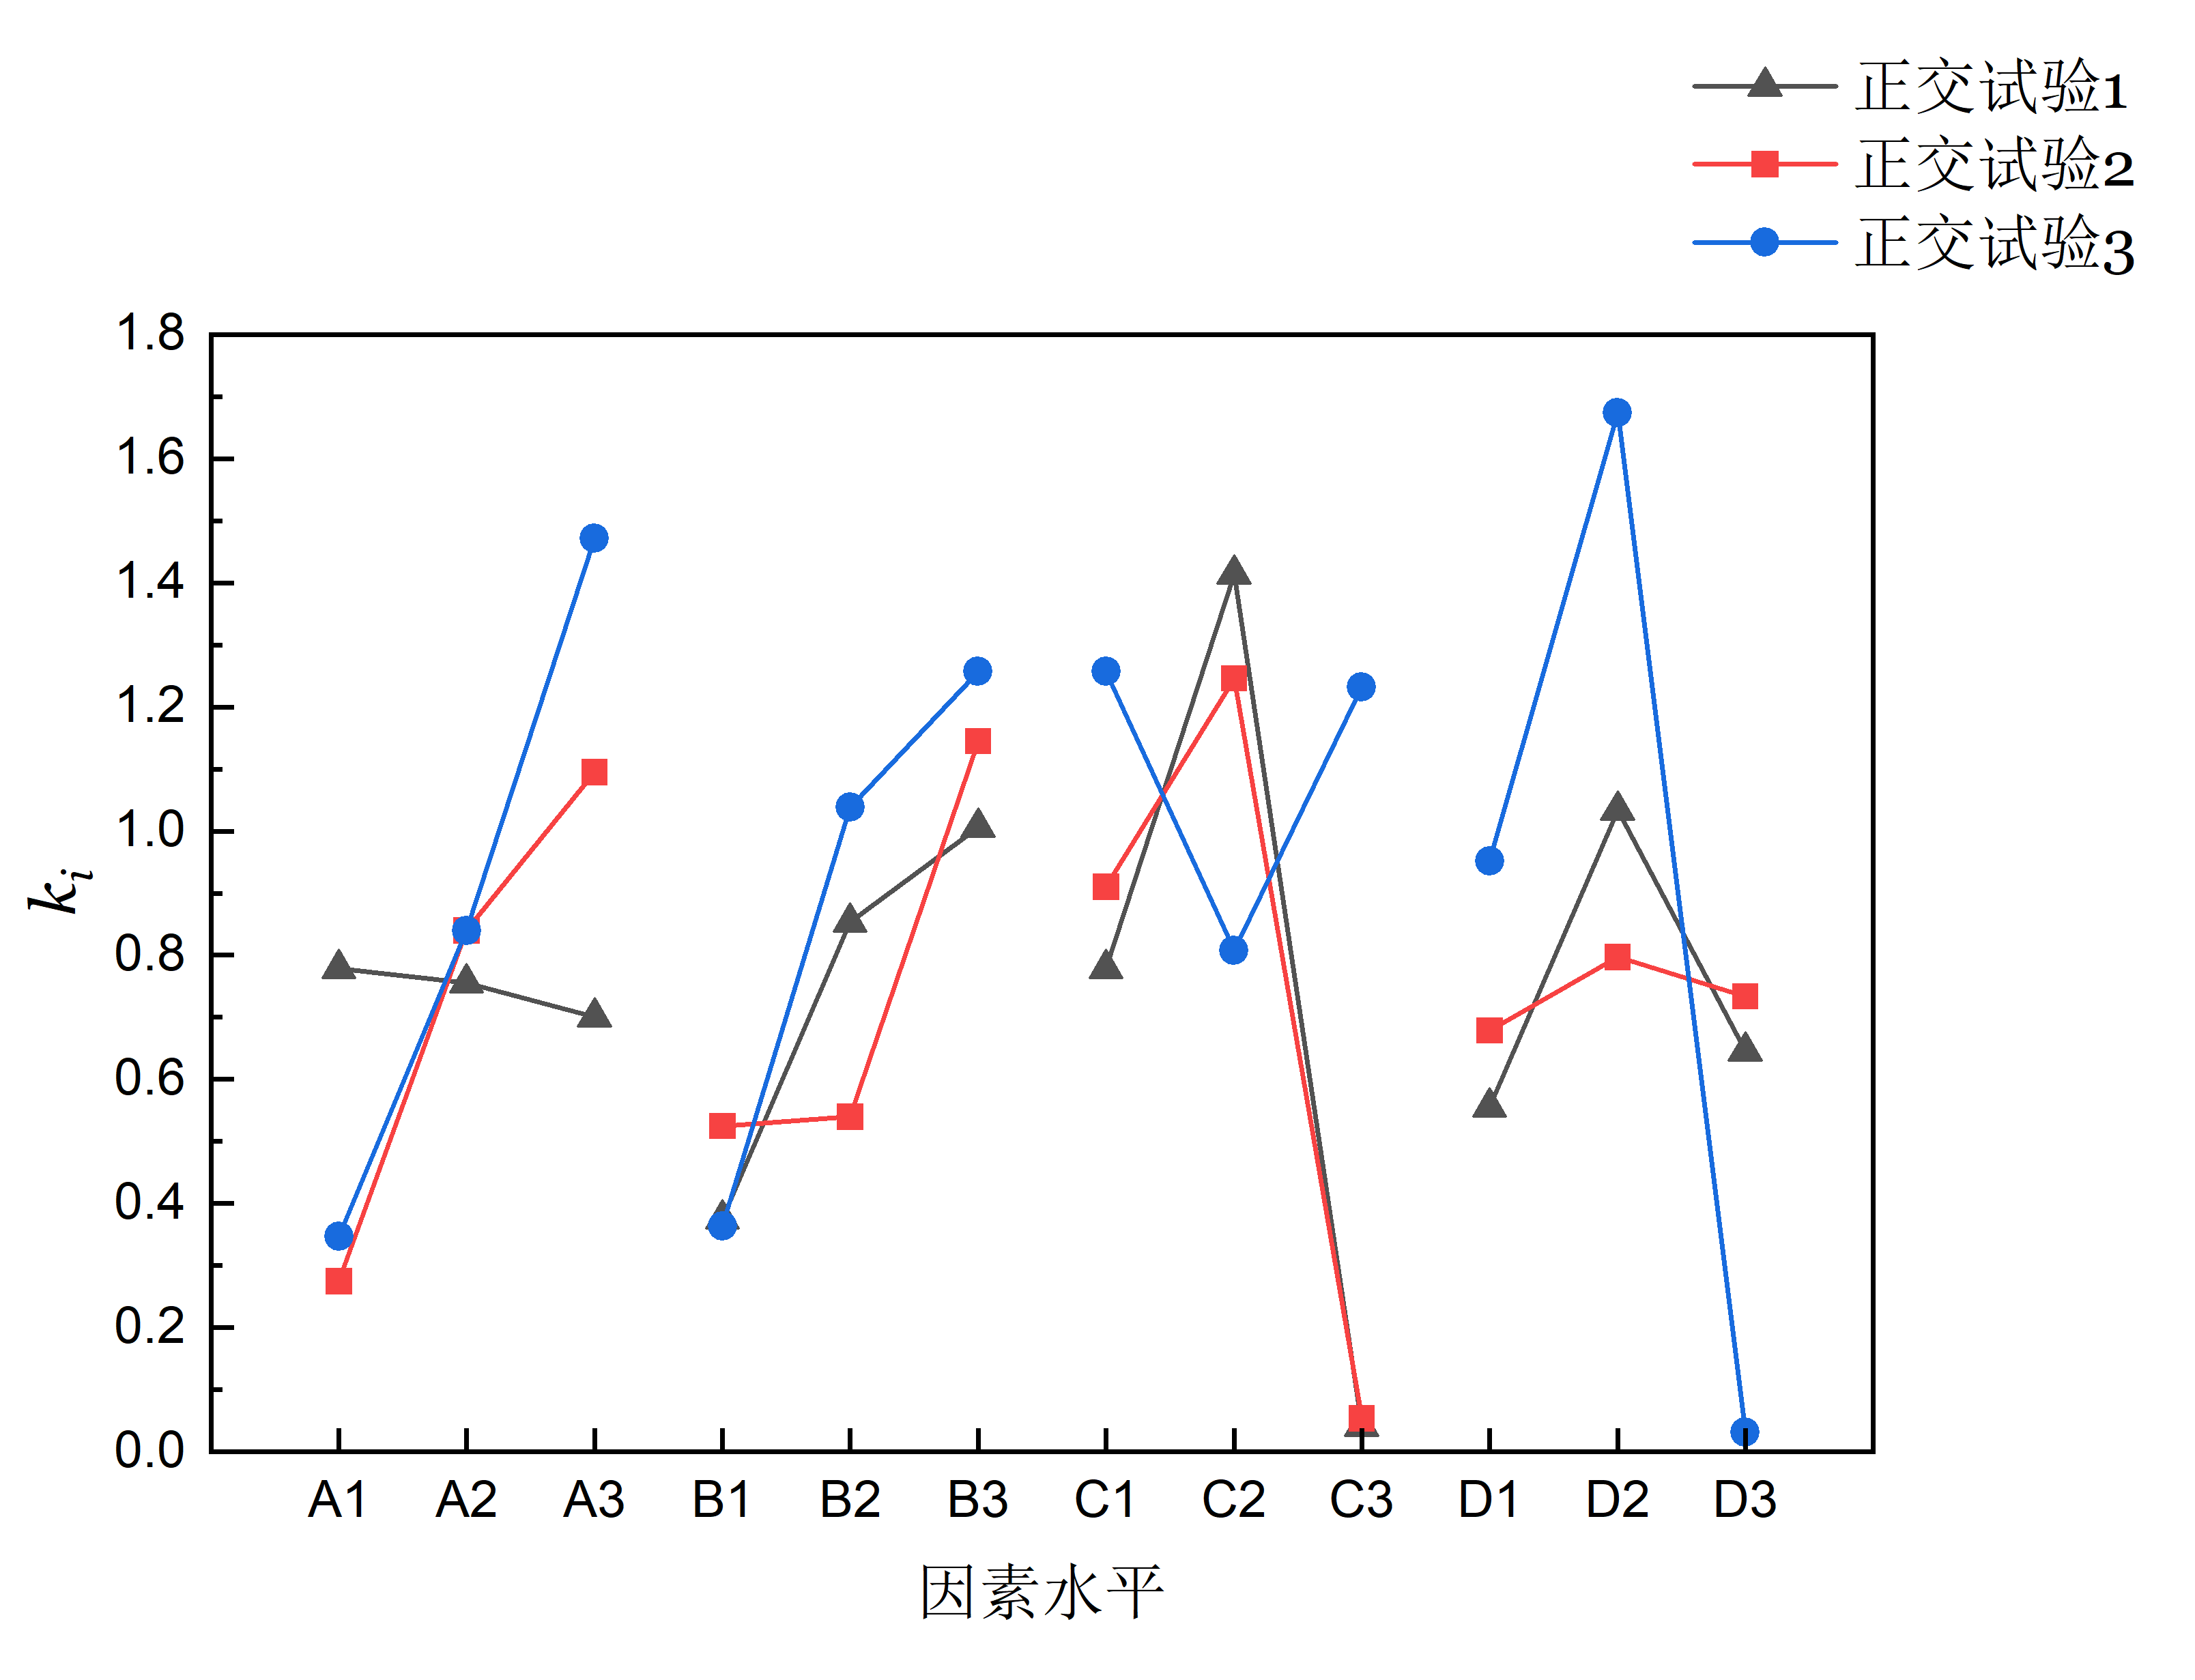
\includegraphics[width = 0.7\textwidth]{figure/Some Pictures/figure-4.png}
    \caption{正交试验的指标-因素关系图}
    \label{fig:enter-label}
\end{figure}

考虑到底物抑制作用和酶用量等相关因素,综合三组试验,确定得最优的条件组合如下表。

% Please add the following required packages to your d\dc ument preamble:
% \usepackage{booktabs}
\begin{table}[H]
\centering
\caption{正交试验确定的最优组合}
\label{tab:my-table}
\begin{tabular}{@{}ccccc@{}}
\toprule
 因素&
  \begin{tabular}[c]{@{}c@{}}{[}S{]}\\ /mL\end{tabular} &
  \begin{tabular}[c]{@{}c@{}}{[}E{]}\\ /mL\end{tabular} &
  \begin{tabular}[c]{@{}c@{}}温度\\ /\dc\end{tabular} &
  pH \\ \midrule
最优组合 &
  0.50 &
  0.037 &
  50 &
  4.6 \\ \bottomrule
\end{tabular}
\end{table}

\subsection{SDS-PAGE}
\par 根据marker条带拟合$\ln M - R_\text{f}$标准曲线如\ref{fig:SDS_STD},与之对比可以推知分离出蛋白质的分子量。从条带灰度曲线图知,分子量小于130kD的蛋白占主要成分,随分离纯化的进行,蛋白质含量逐渐降低,而样品$\mathrm{IV}$中保留了少量126kD蛋白,其余蛋白主要集中在46-79kD,以及大量32kD以下的小分子杂蛋白。酶切样品中126kD蛋白较少,而是转变为85-100kD的蛋白,其余部分与样品$\mathrm{IV}$大致相同。

\begin{figure}
    \subfloat[实验结果图]{
    \label{fig:SDS_Result}
    \includegraphics[width = 0.53\textwidth]{figure/Electro/sds page 图.jpg}
    }
    \subfloat[$\ln M - R_\text{f}$标准曲线]{
    \label{fig:SDS_STD}
    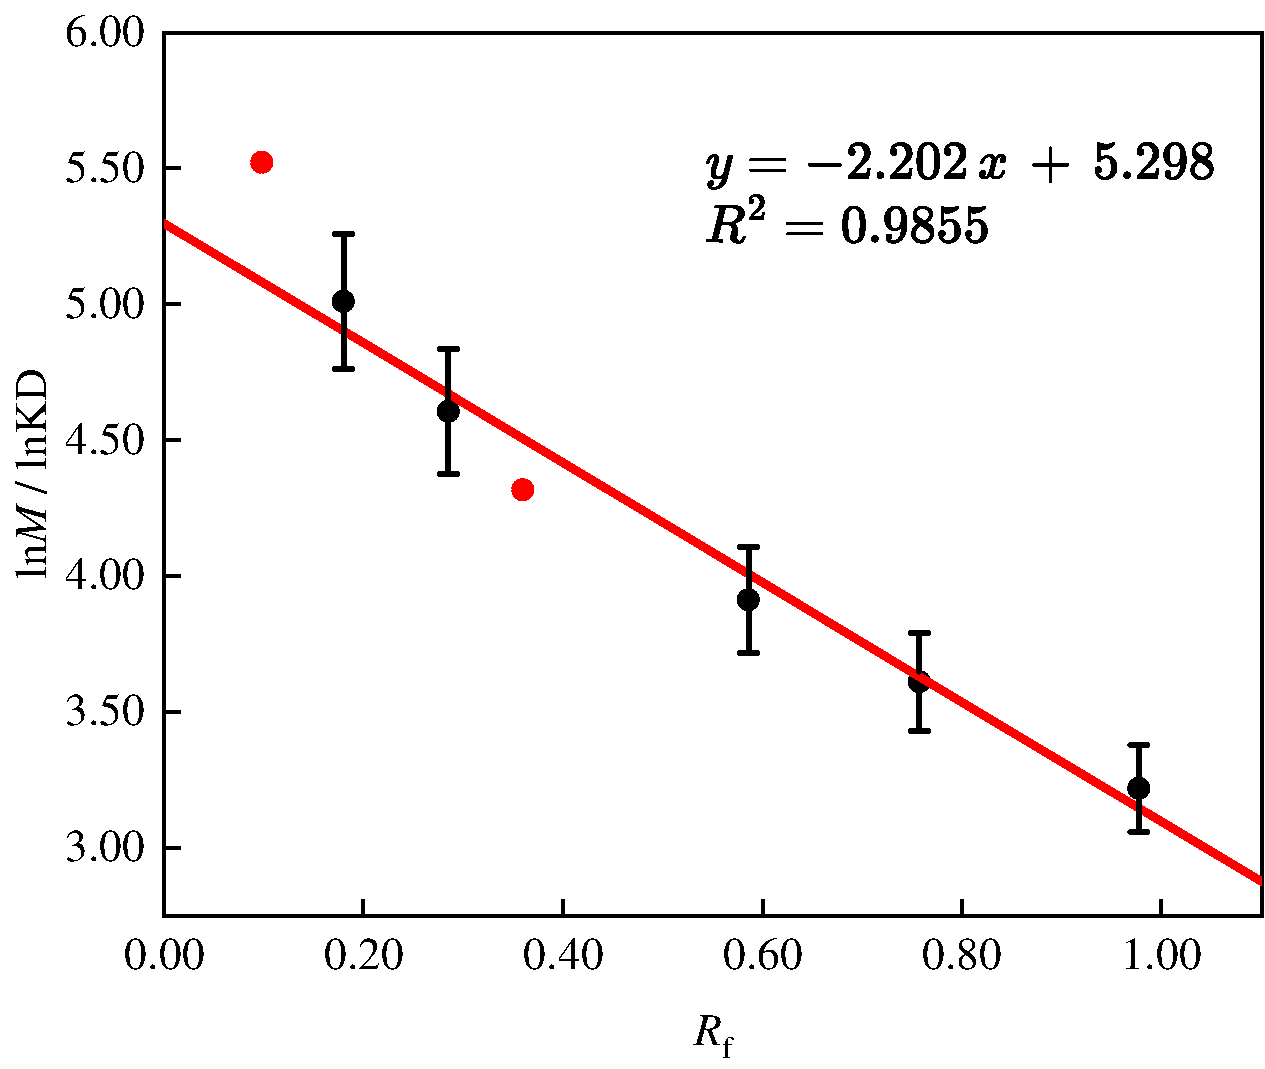
\includegraphics[width = 0.45\textwidth]{figure/Electro/SDS_STD.pdf}
    }
    \caption{蔗糖酶SDS-PAGE电泳}
    \label{fig:SDS-PAGE}
\end{figure}
% \begin{figure}[H]
%     \centering
%     \caption{蔗糖酶SDS-PAGE电泳}
%     \label{fig:4.6.1}
%     \includegraphics[width = 0.8\textwidth]{figure/logo/sds page 图.jpg}
% \end{figure}
\begin{table}[H]
\centering
\caption{SDS-PAGE中Marker分子量及其对数与$R_\text{f}$}
\label{tab:SDS-PAGE_marker}
\begin{tabular}{@{}ccc@{}}
\toprule
$R_\text{f}$    & M/kD & lnM   \\ \midrule
0.098 & 250  & 5.521 \\
0.180 & 150  & 5.011 \\
0.285 & 100  & 4.605 \\
0.360 & 75   & 4.317 \\
0.586 & 50   & 3.912 \\
0.757 & 37   & 3.611 \\
0.977 & 25   & 3.219 \\ \bottomrule
\end{tabular}
\end{table}
% \begin{table}[H]
% \centering
% \caption{SDS PAGE 电泳分子量比移值对数关系}
% \label{46}
% \begin{tabular}{@{}llllll@{}}
% \toprule
% \multicolumn{1}{c}{}       & \multicolumn{1}{c}{$R_\text{f}$}    & \multicolumn{1}{c}{M/kD} & \multicolumn{1}{c}{lnM}   &  &  \\ \midrule
% \multicolumn{1}{c}{marker} & \multicolumn{1}{c}{0.098} & \multicolumn{1}{c}{250}  & \multicolumn{1}{c}{5.521} &  &  \\
% \multicolumn{1}{c}{marker} & \multicolumn{1}{c}{0.18}  & \multicolumn{1}{c}{150}  & \multicolumn{1}{c}{5.011} &  &  \\
% \multicolumn{1}{c}{marker} & \multicolumn{1}{c}{0.285} & \multicolumn{1}{c}{100}  & \multicolumn{1}{c}{4.605} &  &  \\
% \multicolumn{1}{c}{marker} & \multicolumn{1}{c}{0.36}  & \multicolumn{1}{c}{75}   & \multicolumn{1}{c}{4.317} &  &  \\
% \multicolumn{1}{c}{marker} & \multicolumn{1}{c}{0.586} & \multicolumn{1}{c}{50}   & \multicolumn{1}{c}{3.912} &  &  \\
% \multicolumn{1}{c}{marker} & \multicolumn{1}{c}{0.757} & \multicolumn{1}{c}{37}   & \multicolumn{1}{c}{3.611} &  &  \\
% \multicolumn{1}{c}{marker} & \multicolumn{1}{c}{0.977} & \multicolumn{1}{c}{25}   & \multicolumn{1}{c}{3.219} &  &  \\
% \multicolumn{1}{c}{}       & \multicolumn{1}{c}{}      & \multicolumn{1}{c}{}     & \multicolumn{1}{c}{}      &  &  \\ \bottomrule
% \end{tabular}
% \end{table}

\subsection{糖蛋白电泳}
\par 主要条带集中在216kD左右,由于$R_\text{f}$较小,分离不彻底,其余条带还出现于40kD以下,但含量较低。对于216kD条带,样品$\mathrm{I}$、$\mathrm{II}$、$\mathrm{III}$中糖基化蛋白含量高,而样品$\mathrm{IV}$中检测到糖蛋白含量明显降低,知经过柱色谱纯化,去除了大量糖基化的杂蛋白。

\begin{figure}
    \subfloat[实验结果图]{
    \label{fig:SDS_Result}
    \includegraphics[width = 0.52\textwidth]{figure/Electro/糖蛋白电泳图.jpg}
    }
    \subfloat[$\ln M - R_\text{f}$标准曲线]{
    \label{fig:EN_Result}
    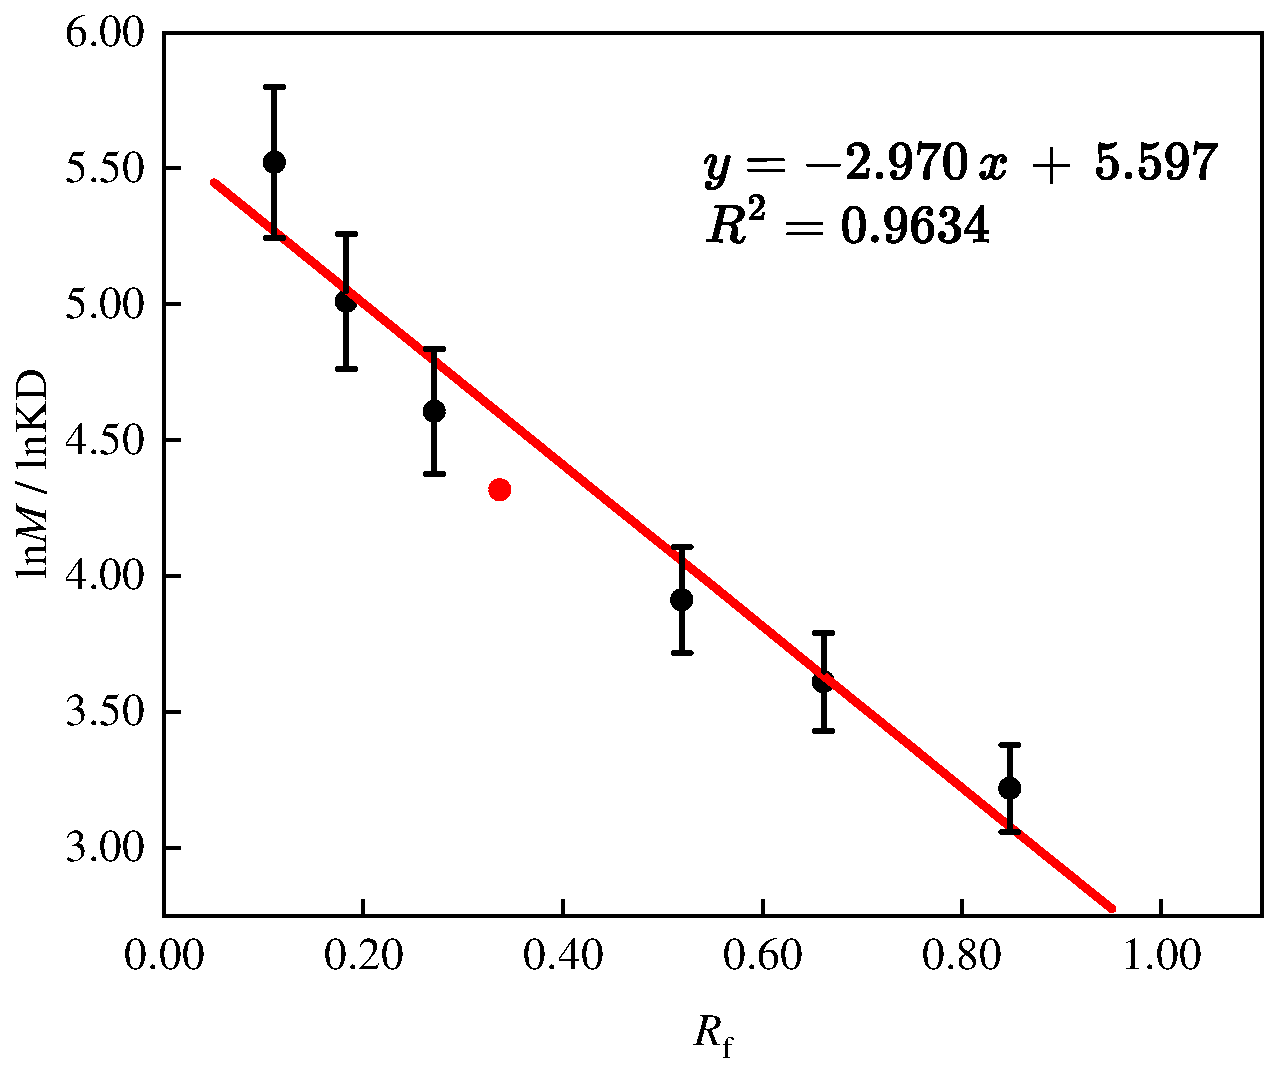
\includegraphics[width = 0.47\textwidth]{figure/Electro/EN_STD.pdf}
    }
    \caption{蔗糖酶糖蛋白电泳}
    \label{fig:EN}
\end{figure}

% \begin{figure}[H]
%     \centering
%     \caption{蔗糖酶糖蛋白电泳}
%     \label{fig:4.7.1}
%     \includegraphics[width = 0.8\textwidth]{figure/logo/糖蛋白电泳图.jpg}
% \end{figure}
\begin{table}[]
\centering
\caption{糖蛋白电泳灰度分析}
\label{tab:}
\begin{tabular}{@{}cccccc@{}}
\toprule
样品编号                                               & 条带  & Peak $R_\text{f}$ & Peak value & Raw volume & $M_r$/kD \\ \midrule
\multirow{7}{*}{样品$\mathrm{I}$}                               & 条带1 & 0.144   & 71         & 64         & 172   \\
                                                   & 条带2 & 0.201   & 83         & 175        & 149   \\
                                                   & 条带3 & 0.221   & 76         & 54         & 142   \\
                                                   & 条带4 & 0.324   & 48         & 21         & 109   \\
                                                   & 条带5 & 0.394   & 54         & 135        & 91    \\
                                                   & 条带6 & 0.426   & 51         & 29         & 84    \\
                                                   & 条带7 & 0.619   & 53         & 12         & 52    \\ \midrule
\multirow{3}{*}{样品$\mathrm{II}$}                               & 条带1 & 0.192   & 58         & 41         & 153   \\
                                                   & 条带2 & 0.204   & 58         & 41         & 148   \\
                                                   & 条带3 & 0.886   & 58         & 12         & 26    \\ \midrule
\multirow{4}{*}{样品$\mathrm{III}$}                               & 条带1 & 0.179   & 64         & 25         & 158   \\
                                                   & 条带2 & 0.187   & 64         & 15         & 154   \\
                                                   & 条带3 & 0.617   & 73         & 18         & 52    \\
                                                   & 条带4 & 0.884   & 67         & 65         & 26    \\ \midrule
\multirow{3}{*}{样品$\mathrm{IV}$}                               & 条带1 & 0.136   & 51         & 49         & 176   \\
                                                   & 条带2 & 0.199   & 63         & 32         & 150   \\
                                                   & 条带3 & 0.216   & 62         & 59         & 144   \\ \midrule
\begin{tabular}[c]{@{}c@{}}样品$\mathrm{IV}$\\ (酶切)\end{tabular} & 条带1 & 0.888   & 73         & 21         & 26    \\ \bottomrule
\end{tabular}
\end{table}
% \begin{table}[]
% \centering
% \caption{糖蛋白电泳灰度分析}
% \label{48}
% \begin{tabular}{@{}cccccc@{}}
% \toprule
%                      &     & Peak $R_\text{f}$ & Peak value & Raw volume & Mr/kD \\ \midrule
% \multirow{5}{*}{样品$\mathrm{I}$} & 条带1 & 0.059   & 203        & 2338       & 213   \\
%                      & 条带2 & 0.695   & 92         & 22         & 33    \\
%                      & 条带3 & 0.746   & 91         & 8          & 29    \\
%                      & 条带4 & 0.796   & 93         & 16         & 25    \\
%                      & 条带5 & 0.852   & 107        & 161        & 21    \\
% \multirow{4}{*}{样品$\mathrm{II}$} & 条带1 & 0.053   & 195        & 3562       & 217   \\
%                      & 条带2 & 0.702   & 91         & 13         & 33    \\
%                      & 条带3 & 0.803   & 95         & 18         & 24    \\
%                      & 条带4 & 0.851   & 105        & 35         & 21    \\
% \multirow{4}{*}{样品$\mathrm{III}$} & 条带1 & 0.056   & 186        & 2628       & 215   \\
%                      & 条带2 & 0.214   & 112        & 7          & 136   \\
%                      & 条带3 & 0.739   & 96         & 34         & 29    \\
%                      & 条带4 & 0.857   & 103        & 14         & 21    \\
% \multirow{4}{*}{样品$\mathrm{IV}$} & 条带1 & 0.054   & 128        & 205        & 216   \\
%                      & 条带2 & 0.211   & 110        & 30         & 137   \\
%                      & 条带3 & 0.611   & 95         & 27         & 43    \\
%                      & 条带4 & 0.728   & 94         & 7          & 30    \\
% \multicolumn{1}{l}{} & \multicolumn{1}{l}{} & \multicolumn{1}{l}{} & \multicolumn{1}{l}{} & \multicolumn{1}{l}{} & \multicolumn{1}{l}{} \\ \bottomrule
% \end{tabular}
% \end{table}

\subsection{活性蛋白电泳}
\par 各样品均有227kD附近的条带出现,由于$R_\text{f}$较小,分离不彻底,可能含有多种分子量接近的蛋白质,而在样品$\mathrm{I,II,III}$中还有64kD的条带,但在纯化后的样品$\mathrm{IV}$中没有发现;酶切样品中条带下移,可见去除糖链后蛋白电泳时移动性更好。

\begin{figure}
    \subfloat[实验结果图]{
    \label{fig:SDS_Result}
    \includegraphics[width = 0.50\textwidth]{figure/Electro/活性电泳图.jpg}
    }
    \subfloat[$\ln M - R_\text{f}$标准曲线]{
    \label{fig:AC_Result}
    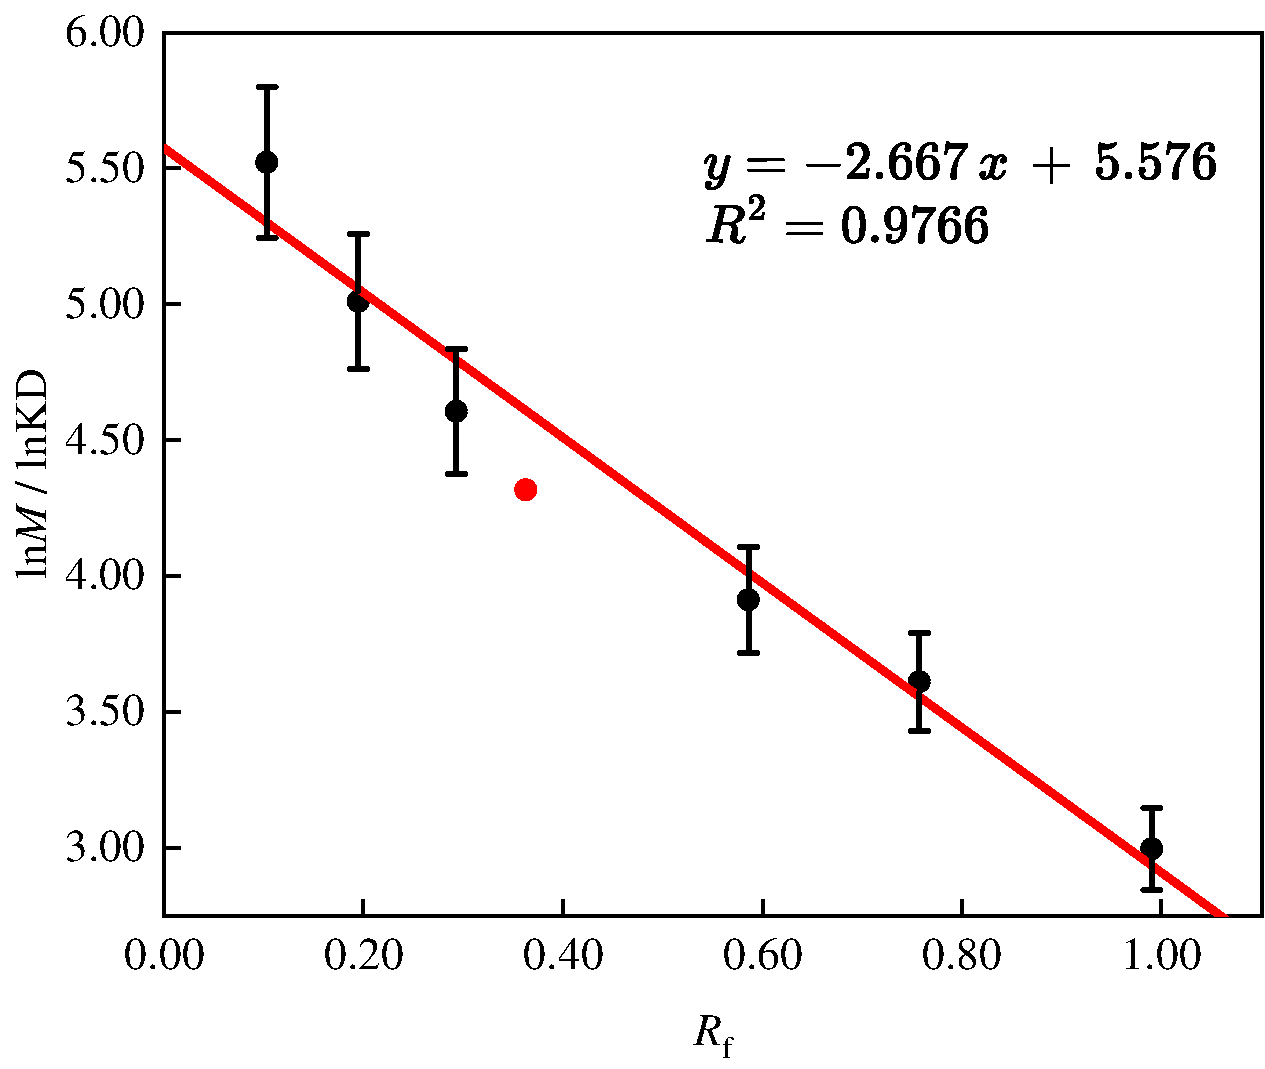
\includegraphics[width = 0.46\textwidth]{figure/Electro/AC_STD.pdf}
    }
    \caption{蔗糖酶活性电泳}
    \label{fig:AC}
\end{figure}

% \begin{figure}[H]
%     \centering
%     \caption{蔗糖酶活性电泳}
%     \label{fig:4.8.1}
%     \includegraphics[width = 0.8\textwidth]{figure/logo/活性电泳图.jpg}
% \end{figure}

\begin{table}[]
\centering
\caption{活性电泳条带灰度分析}
\label{481}
\begin{tabular}{@{}cccccl@{}}
\toprule
                     &                      & Peak $R_\text{f}$              & Peak value           & Raw volume           &  \\ \midrule
\multirow{3}{*}{样品$\mathrm{I}$} & 条带1                  & 0.029                & 141                  & 45                   &  \\
                     & 条带2                  & 0.515                & 88                   & 25                   &  \\
                     & 条带3                  & 0.981                & 75                   & 10                   &  \\  \midrule
\multirow{3}{*}{样品$\mathrm{II}$} & 条带1                  & 0.036                & 141                  & 25                   &  \\
                     & 条带2                  & 0.514                & 94                   & 22                   &  \\
                     & 条带3                  & 0.991                & 77                   & 20                   &  \\  \midrule
\multirow{2}{*}{样品$\mathrm{III}$} & 条带1                  & 0.031                & 138                  & 50                   &  \\
                     & 条带2                  & 0.512                & 91                   & 32                   &  \\  \midrule
样品 $\mathrm{IV}$                 & 条带1                  & 0.043                & 193                  & 50                   &  \\
 \bottomrule
\end{tabular}
\end{table}

\begin{table}[]
\centering
\caption{活性电泳条带灰度分析}
\label{tab:Actibity_Electro}
\begin{tabular}{@{}cccccc@{}}
\toprule
样品编号                 & 条带  & Peak Rf & Peak value & Raw volume & Mr/kD \\ \midrule
\multirow{3}{*}{样品$\mathrm{I}$} & 条带1 & 0.029   & 141        & 45         & 244   \\
                     & 条带2 & 0.515   & 88         & 25         & 67    \\
                     & 条带3 & 0.981   & 75         & 10         & 19    \\ \midrule
\multirow{3}{*}{样品$\mathrm{II}$} & 条带1 & 0.036   & 141        & 25         & 240   \\
                     & 条带2 & 0.514   & 94         & 22         & 67    \\
                     & 条带3 & 0.991   & 77         & 20         & 19    \\ \midrule
\multirow{2}{*}{样品$\mathrm{III}$} & 条带1 & 0.031   & 138        & 50         & 243   \\
                     & 条带2 & 0.512   & 91         & 32         & 67    \\ \midrule
样品$\mathrm{IV}$                  & 条带1 & 0.043   & 193        & 50         & 235   \\ \bottomrule
\end{tabular}
\end{table}

\subsection{Western Blot}
\par 由Western Blot结果知,样品中含有130-160kD蛋白质,样品$\mathrm{I}$中86kD左右蛋白经过热处理后被去除。样品$\mathrm{IV}$中小分子量的杂蛋白含量降低。样品酶切后蛋白含量下降,未检测出相应条带。
% Please add the following required packages to your d\dc ument preamble:
% \usepackage{booktabs}
% \usepackage{multirow}
\begin{table}[]
\centering
\caption{WB条带灰度分析}
\label{491}
\begin{tabular}{@{}cccccl@{}}
\toprule
                     &     & Peak $R_\text{f}$ & Peak value & Raw volume &  \\ \cmidrule(lr){1-5}
\multirow{7}{*}{样品$\mathrm{I}$} & 条带1 & 0.144   & 71         & 64         &  \\
                     & 条带2 & 0.201   & 83         & 175        &  \\
                     & 条带3 & 0.221   & 76         & 54         &  \\
                     & 条带4 & 0.324   & 48         & 21         &  \\
                     & 条带5 & 0.394   & 54         & 135        &  \\
                     & 条带6 & 0.426   & 51         & 29         &  \\
                     & 条带7 & 0.619   & 53         & 12         &  \\  \cmidrule(lr){1-5}
\multirow{3}{*}{样品$\mathrm{II}$} & 条带1 & 0.192   & 58         & 41         &  \\
                     & 条带2 & 0.204   & 58         & 41         &  \\
                     & 条带3 & 0.886   & 58         & 12         &  \\  \cmidrule(lr){1-5}
\multirow{4}{*}{样品$\mathrm{III}$} & 条带1 & 0.179   & 64         & 25         &  \\
                     & 条带2 & 0.187   & 64         & 15         &  \\
                     & 条带3 & 0.617   & 73         & 18         &  \\
                     & 条带4 & 0.884   & 67         & 65         &  \\  \cmidrule(lr){1-5}
\multirow{3}{*}{样品$\mathrm{IV}$} & 条带1 & 0.136   & 51         & 49         &  \\
                     & 条带2 & 0.199   & 63         & 32         &  \\
                     & 条带3 & 0.216   & 62         & 59         &  \\  \cmidrule(lr){1-5}
样品$\mathrm{IV}$(酶切)              & 条带1 & 0.888   & 73         & 21         & \\ \cmidrule(lr){1-5}
\end{tabular}
\end{table}

\begin{figure}
    \subfloat[实验结果图]{
    \label{fig:SDS_Result}
    \includegraphics[width = 0.53\textwidth]{figure/Electro/wb图.jpg}
    }
    \subfloat[$\ln M - R_\text{f}$标准曲线]{
    \label{fig:AC_Result}
    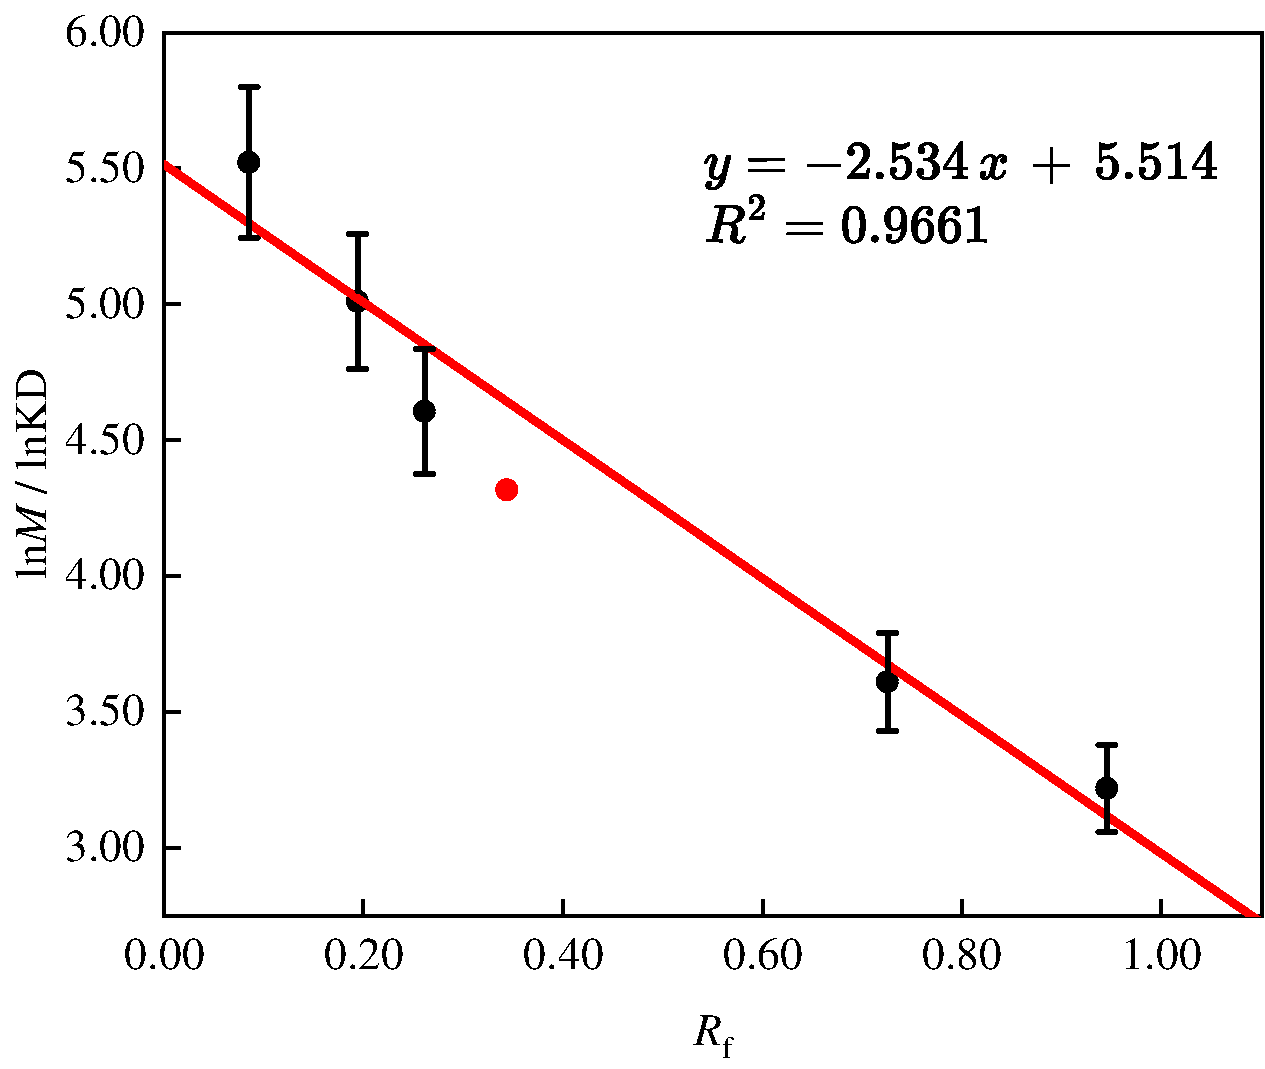
\includegraphics[width = 0.45\textwidth]{figure/Electro/WB_STD.pdf}
    }
    \caption{蔗糖酶活性电泳}
    \label{fig:WB}
\end{figure}        
% \begin{figure}[H]
%     \centering
%     \caption{蔗糖酶Western Blot检测}
%     \label{fig:4.9.1}
%     \includegraphics[width = 0.8\textwidth]{figure/logo/wb图.jpg}
% \end{figure}
\subsection{酶促反应动力学}


\section{分析与讨论}

\subsection{蔗糖酶的分离与纯化}
经破碎、热处理、乙醇沉淀和复性溶解等步骤对酵母细胞中的外蔗糖酶进行提取和粗分离,并使用阴离子交换柱色谱进行纯化,通过自动收集器收集到了一系列样本溶液。使用3,5-二硝基水杨酸法检验蔗糖酶的活性,观察发现18号管的颜色最深,说明该管可能为酶活性最高管。由于肉眼观察存在一定的局限性,加之18号管附近的样品管颜色差异不明显,因此可通过分光光度法测定吸光度等定量的方法进一步确定酶活性最高管,作为样品IV参与后续实验。同时,在破壁粗提、热处理、乙醇沉淀与复性溶解三个节点收集了样本I、样本II、样本III,也对阴离子交换柱色谱穿流峰洗脱时的产物进行留样。

生物化学实验是我们现阶段所接触到的最接近于科研工作的课程。通过具有连贯性的实验设计和实际执行,我们学习了基本的实验操作和分析技能,深入思考实验背后的原理和逻辑,为今后的科研生活奠定坚实的基础。而正确、规范的实验操作是保证实验准确性和可信度的必要前提。在蔗糖酶的提取和粗分离的过程中,史锋老师一针见血地指出了我们在研磨过程中存在的技术错误,并为我们示范了规范的操作方法,从而保证了粗提取的有效性。并且,两位老师一直在强调做实验不能只停留在“做”的层面,而是应该“动动脑筋”,深入思考,从“怎么做”、“为什么这样做”到“如何做会更好”,只有自己真正掌握了实验背后的原理和逻辑,才能真正有所收获、有所成长,而不是一味照搬式地操作,出现错误的甚至威胁实验室安全的行为。

\subsection{蛋白质浓度测定}

\subsection{酶活性的测定}
\par 使用DNS法分光光度定量检测蔗糖酶活性,对保温时间的严格控制是保证结果可信度的关键,也是方法误差的一个主要来源。此外,分光光度计系统误差也对吸光度检测造成一定的影响。
\subsection{蔗糖酶酶切去糖基化}

\subsection{正交试验探究最佳反应条件}

\subsection{SDS-PAGE}

\subsection{糖蛋白电泳}

\subsection{活性蛋白电泳}

\subsection{Western Blot}

\subsection{酶促反应动力学}

% \section{蔗糖酶提取和粗分离、离子交换树脂色谱}

% \subsection{实验材料与仪器}

% \subsection{实验步骤}

% \subsection{实验结果与数据}
%
% \subsection{实验结果分析与讨论}

% \section{纯化方案评价设计}

% \subsection{实验原理}

% \subsection{实验材料与仪器}

% \subsection{实验步骤}


% \subsection{实验结果与数据}
% \begin{figure}[ht]
%     \centering
%     \caption{蔗糖酶洗脱曲线}
%     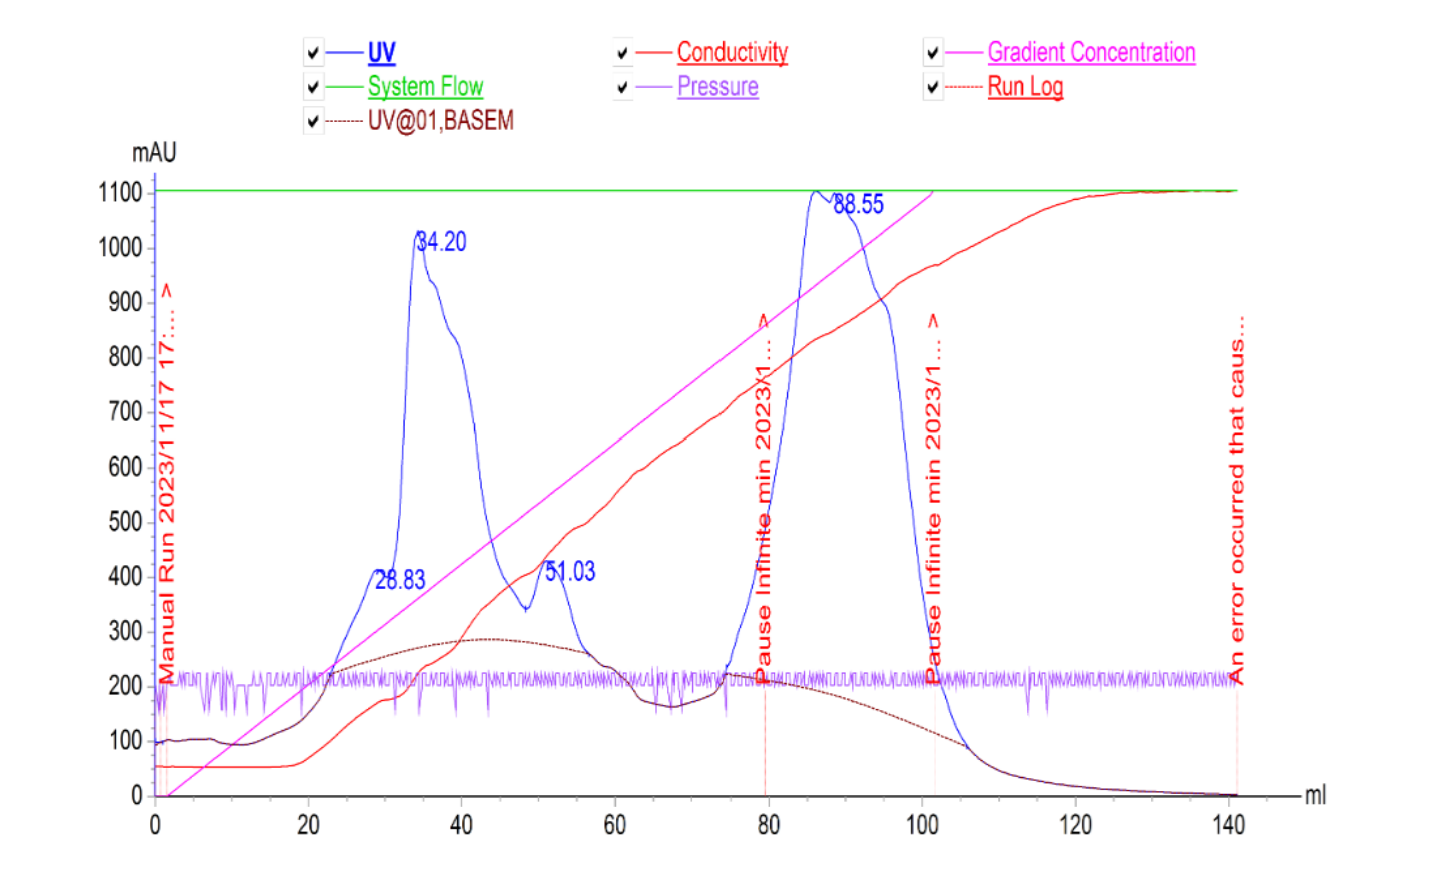
\includegraphics[width = 0.8\textwidth]{figure/logo/curve.png}
% \end{figure}


% \subsection{实验结果分析与讨论}



% \section{Overleaf 使用注意事项}

% \ce{CH3COOH}

% 如\autoref{tab:my-table}

% % \begin{longtable}[c]{ccccc}
% % \caption{result}
% % \label{tab:my-table}\\
% % \hline
% % 组别                       & 完整细胞数 & 细胞融合数 & 融合比例/\% & 平均融合比率/\%              \\ \hline
% % \endfirsthead
% % %
% % \multicolumn{5}{c}%
% % {{\bfseries Table \thetable\ continued from previous page}} \\
% % \endhead
% % %
% % \hline
% % \endfoot
% % %
% % \endlastfoot
% % %
% % \multirow{5}{*}{Control} & 155   & 6     & 3.87    & \multirow{5}{*}{2.76}  \\
% %                          & 151   & 4     & 2.65    &                        \\
% %                          & 146   & 4     & 2.74    &                        \\
% %                          & 158   & 2     & 1.27    &                        \\
% %                          & 153   & 5     & 3.27    &                        \\ \hline
% % \multirow{5}{*}{PEG}     & 68    & 10    & 14.71   & \multirow{5}{*}{14.07} \\
% %                          & 60    & 9     & 15.00   &                        \\
% %                          & 64    & 9     & 14.06   &                        \\
% %                          & 57    & 7     & 12.28   &                        \\
% %                          & 63    & 9     & 14.29   &                        \\ \hline
% % \multirow{5}{*}{50\%PEG} & 197   & 24    & 12.18   & \multirow{5}{*}{12.11} \\
% %                          & 180   & 20    & 11.11   &                        \\
% %                          & 178   & 23    & 12.92   &                        \\
% %                          & 182   & 22    & 12.09   &                        \\
% %                          & 196   & 24    & 12.24   &                        \\ \hline
% % \end{longtable}


% 如果你在Overleaf上编译本模板,请注意如下事项~\cite{zjuthesis}:

% \begin{itemize}
%     \item 删除根目录的 ``.latexmkrc'' 文件,否则编译失败且不报任何错误
%     \item 字体有版权所以本模板不能附带字体,请务必手动上传字体文件,并在各个专业模板下手动指定字体。
%         具体方法参照 GitHub 主页的说明。
%     \item 当前(2019年9月2日)的Overleaf使用TexLive 2017进行编译,但一些伪粗体复制乱码的问题需要TexLive 2019版本来解决。
%         所以各位同学可以在Overleaf上编写论文,但务必使用本地的TexLive 2019来进行最终编译,以免产生查重相关问题。
%         具体说明参照 GitHub 主页。
% \end{itemize}

% \subsection{节标题}

% \subsubsection{小节标题}

% \par 我们可以用includegraphics来插入现有的jpg等格式的图片,如\autoref{fig:zju-logo}。

% \begin{figure}[ht]
%     \centering
%     \caption{浙江大学}
%     
\includegraphics[width = 0.8\textwidth]{figure/logo/zjuchar.pdf}
% \end{figure}

% \begin{figure}[ht]
%     \centering
%     
\includegraphics[width=.4\linewidth]{logo/zju}
%     \caption{\label{fig:zju-logo}浙江大学LOGO}
% \end{figure}

% \par 如\autoref{tab:sample}所示,这是一张自动调节列宽的表格。

% \begin{table}[ht]
%     \caption{\label{tab:sample}自动调节列宽的表格}
%     \begin{tabularx}{\linewidth}{|c|X<{\centering}|}
%         \hline
%         第一列 & 第二列 \\ \hline
%         xxx & xxx \\ \hline
%         xxx & xxx \\ \hline
%         xxx & xxx \\ \hline
%     \end{tabularx}
% \end{table}

% \par 如\autoref{equ:sample},这是一个公式

% \begin{equation}
%     \label{equ:sample}
%     A=\overbrace{(a+b+c)+\underbrace{i(d+e+f)}_{\text{虚数}}}^{\text{复数}}
% \end{equation}

% \par 如\autoref{code:sample}所示,这是一段代码。
% 计算机学院的代码样式可能与其他专业不同,
% 如有需要,可以从计算机学院专业模板中复制相关的代码样式设定。

% \begin{lstlisting}[%
%     language={C},
%     caption={simple.c},
%     label={code:sample}
% ]
% #include <stdio.h>

% int main(int argc, char *argv[])
% {
%     printf("Hello, zjuthesis\n");
%     return 0;
% }
% \end{lstlisting}

% \subsection{关于字体}

% 英文字体通常提供了粗体和斜体的组合,中文字体通常没有粗体或斜体,本模板使用了 `AutoFakeBold' 来实现中文伪粗体,但不提供中文斜体,如\autoref{tab:font-examples}所示。

% \begin{table}
%     \centering
%     \caption{一些字体示例}
%     \label{tab:font-examples}
%     \begin{tabular}{|c|c|c|c|c|}
%         \hline
%         字体            & 常规             & 粗体                       & 斜体                      & 粗斜体                                \\ \hline
%         Times New Roman & Regular         & {\bfseries          Bold} & {\itshape         Italic} & {\bfseries \itshape      BoldItalic} \\ \hline
%         仿宋            & {\fangsong 常规} & {\fangsong \bfseries 粗体} & {\fangsong \itshape 斜体} & {\fangsong \bfseries \itshape 粗斜体} \\ \hline
%         宋体            & {\songti   常规} & {\songti   \bfseries 粗体} & {\songti   \itshape 斜体} & {\songti   \bfseries \itshape 粗斜体} \\ \hline
%         黑体            & {\heiti    常规} & {\heiti    \bfseries 粗体} & {\heiti    \itshape 斜体} & {\heiti    \bfseries \itshape 粗斜体} \\ \hline
%         楷体            & {\kaishu   常规} & {\kaishu   \bfseries 粗体} & {\kaishu   \itshape 斜体} & {\kaishu   \bfseries \itshape 粗斜体} \\ \hline
%     \end{tabular}
% \end{table}

% \sectionnonum[none]{同一页上的章标题}
